 \documentclass[11pt,titlepage,a5paper]{book}

% \usepackage[babel,german=quotes]{csquotes}
 
 \usepackage[ngerman]{babel}
  \usepackage[utf8]{inputenc}
  \usepackage[T1]{fontenc}


 \usepackage{graphicx}
 \usepackage{geometry}
 \usepackage{pstricks}
 
% \usepackage[style=numeric-comp,backend=bibtex]{biblatex}
% \addbibresource{Bilbliothek.bib}
 
 \pagestyle{plain}

\clubpenalty3000
\widowpenalty3000
\displaywidowpenalty=3000
 
%\frenchspacing 

\parindent0em 
\setlength{\parskip}{0.4ex plus 0.6ex minus 0.4ex}
\sloppy

\geometry{left=2.5cm,right=2cm,bottom=3.5cm,top=2.0cm}

 \author{von\\[0.8ex]Felicitas Stotz}
 \title{\bf\Huge Die Horussöhne}
 
 \newcommand{\sterne}{\par{\centering ***\par}}
 \newcommand{\ti}{"`}
 \newcommand{\ho}{"'}

 \newenvironment{tg}{\begin{quote}\em}{\end{quote}}
  
 \newenvironment{dichter}{\begin{flushright}}{\end{flushright}}

\newcommand{\changefont}[3]{
\fontfamily{#1} \fontseries{#2} \fontshape{#3} \selectfont}



 \begin{document}
% .
% \newpage
% \newpage
 
 \changefont{ppl}{m}{n}
 
  %\maketitle
   
 \begin{titlepage} 

%\includegraphics[width=0.9\textwidth]{/home/felicitas/133_1.JPG}

\begin{pspicture}
(-4.9,8.5)
\rput(0cm,0cm){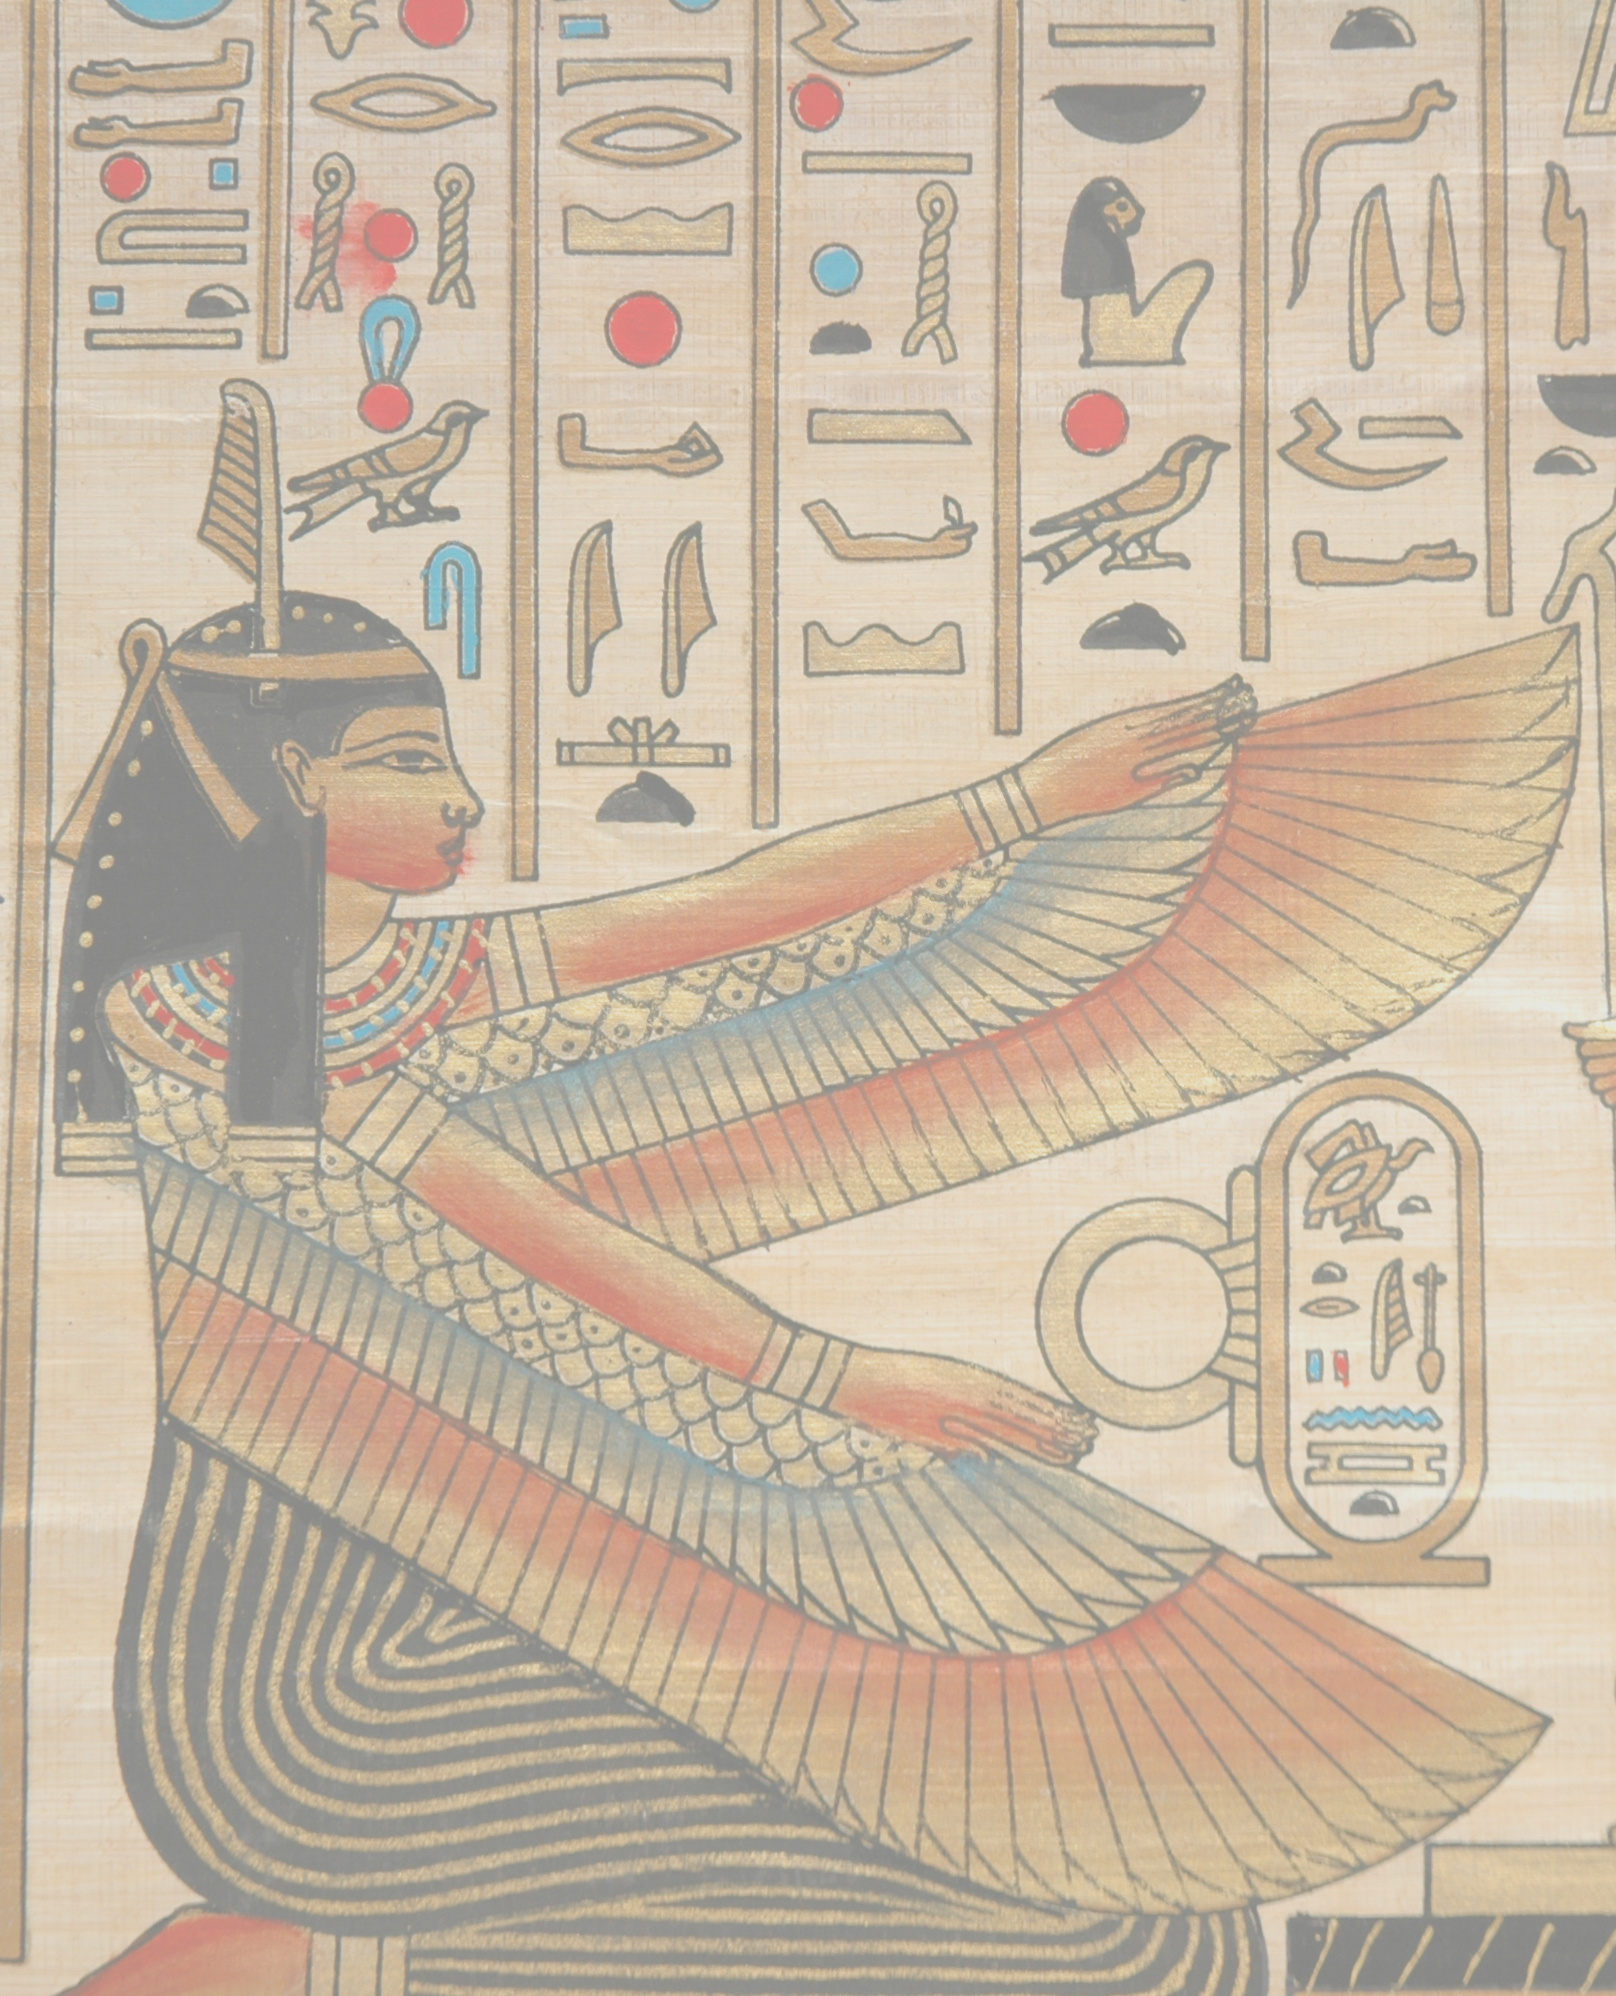
\includegraphics[width=\paperwidth,height=\paperheight]{Titel-Hell}}
\end{pspicture}
  
  \vspace*{-0.4\textheight}
  {\fontsize{40}{60}\selectfont Die Horussöhne}\\[38ex]
  {\huge Felicitas Stotz}\\[8ex]
   \today
 
 \end{titlepage}


\thispagestyle{empty}


\chapter*{}

\section*{Titelei}

\begin{tg}
\begin{verse}



Die Schrift des Verborgenen Raumes.\\
Die Standorte der Bau und der Götter,\\
die Schatten und Achu, und was getan wird.

Der Anfang ist das Horn des Westens,\\
das Tor des Westhorizontes;\\
das Ende ist die Urfinsternis,\\
das Tor des Westhorizontes.

Zu kennen die Unterweltlichen Bau,\\
zu kennen die Geheimen Bau,\\
zu kennen die Tore\\
und die Wege, auf denen der Grösste Gott wandelt.

Zu kennen, was getan wird,\\
zu kennen, was in den Stunden ist, und ihre Götter,\\
zu kennen den Lauf der Stunden, und ihre Götter.


Zu kennen ihre Verklärungen des RE,\\
zu kennen, was er ihnen zuruft,\\
zu kennen die Gedeihenden und die Ver\-nich\-te\-ten.{}\\

\end{verse}
\end{tg}



\chapter*{Eine Nacht im Januar(Prolog)}
\addcontentsline{toc}{chapter}{Prolog: Eine Nacht im Januar}

Die Wahrheit ist: Wir wissen es nicht! 

Was wir wissen, sind die Dinge, die wir wahr-nehmen. Wir nehmen sie mit unseren Sinnen auf und bewerten sie. Dabei bewerten wir sie nach nützlich oder unnütz, essbar oder nicht essbar und kommt es für die Paarung in Frage? Wenn wir die Dinge als wahr bezeichnen, die wir mit den Sinnen in der physischen Welt erfahren, sind wir auf der sichereren Seite. Nicht ganz sicher, aber immerhin\dots

Dann gibt es unser Gehirn, unsere Emotionen, unsere Träume, unsere Hoffnungen und Wünsche, unsere Ängste, unseren Glauben\dots Sie sind unsichtbar, unfassbar, aber denkbar. Das ist interessant, weil wir in unserem Gehirn die sichtbaren Wahrnehmungen und die unsichtbaren Gedanken miteinander untrennbar vermischen. Und weil wir sie vermischen, wissen wir schliesslich nicht mehr, was wir wahrnehmen könnten und was denken. Wissen wir nicht, was wir erfahren haben, was wir kennen und was wir nicht wissen können, weil wir es mit einem grauen, weichen Fleischklops gedacht haben.

Wir neigen dazu, uns für alles eine Antwort zu basteln. Denn eine erklärbare Welt ist eine überschaubare Welt. Eine Welt, in der man weiss, wo der Tiger wohnt\dots \footnote{Eine beliebte Tiger-Adresse ist der indische Dschungel und Sibirien.} Dann kommen wir mit den Unsichtbarkeiten unseres Daseins besser zurecht. Den dunklen Gedanken in der Nacht, wenn wir nicht mehr sicher sind, ob wir wissen, wo der Tiger wohnt.

Und wenn wir die samtweichen Tigerpranken an unserem Schlafpelz vorbei schleichen hören, wünschen wir uns jemanden, der uns beschützt. Einen Krieger! Zwei starke Krieger! Zwanzig starke Krieger!

 Viele, starke Riesenkrieger, die dem Tiger in den Hinter treten und ihn im hohen Bogen bis nach Sibirien schicken, damit wir genau wissen, wo er wohnt und sich seinen  verd***ten, schmerzenden, kalten Hintern schleckt! Weit weg im verd***t Sibirien!
 
Vielleicht, -wir wissen es nicht. Vielleicht sind so die ersten Götter entstanden? => Götter = Tigerschnelllieferservice für die Russen! 

Und wenn wir beginnen unser Gehirn für Erklärungen der Dinge zu bemühen, die wir nicht verstehen, dann könnten wir auf die Idee kommen, der Tigerschnelllieferservice könnte viel mehr.

Vielleicht würden wir die Chance ergreifen und uns vorstellen, dass die starken Riesenkrieger die Welt erschaffen haben. Und wenn sie zusammen schaffen, dann brauchen sie einen Chef! Und wo wohnt der Chef der starken Riesenkrieger, während seine Jungs die Welt bauen? Logisch, auf der Sonne! Die ist ein würdiger Chefsessel! Und wo starke Jungs sind und ein Chef, da dürfen auch die Frauen und Mütter nicht fehlen\dots 

Et voila! Fertig ist die Götterwelt! Gibt es sie, gibt es sie nicht? Wir wissen es nicht. Was wir jedoch wissen und kennen, ist die Sehnsucht die Dinge zu verstehen, die Fäden der Geschichte zu finden, damit wir etwas haben, an dem wir unseren Sinn finden und ihm folgen können. Götter können dafür ein nützliches Konzept bereit halten. Eine gute Erklärung, wieso es die Welt gibt und eine, die die Verantwortlichkeiten klärt.

=> Götter = Weltenerbauer => Verantwortlich = Praktisch\footnote{Sich im Geiste Dinge vorzustellen um Informationen zu bekommen, ist völlig okay. Schliesslich haben wir diese tolle Denkkiste in unserem Kopf. Schwierigkeiten bekommen wir dann, wenn wir uns von unserem exzentrischen Denkkasten Unsichtbarkeiten als Dogmen verkaufen lassen! Also, wenn ein kleiner, grüner Zwerg Dir sagt, was Du tun sollst, dann hör nicht auf ihn. Wenn er Dir jedoch interessante Informationen zukommen lässt, dann brauche sie bei Deiner Entscheidungssuche. Allerdings erst, wenn Du darüber nachgedacht hast.}

Götter sind kreativ und eine ihre beliebtesten Hauptaufgaben ist die Schöpfung. Es gibt viele verschiedene Versionen und Ideen bei den Menschen, wie die Erde in den Zustand gekommen ist, in dem sie sich zur Zeit befindet. Und viele Jahrtausende waren sich unsere Vorfahren einig, es sind Götter gewesen. Einer, viele, egal, aber Götter. Unsichtbare, dem Menschen überlegene Wesen, die alles mehr oder weniger leiteten und im Griff hatten.

Heute, nur am Rande bemerkt, lachen die Menschen über dieses Konzept. Sie glauben nicht an Götter, sondern an die Wissenschaft, was bedeutet, alles hat sich entwickelt. Wie genau das gegangen ist, ist so kompliziert, das verstehen nur wenige. (Früher nannte man die Wenigen mit dem "`geheimen Wissen"' "`Eingeweihte"' und dieses Wissen wurde eifersüchtig von ihnen gehütet, aber das war früher. Ha! Hahaha! Heute nennt man es Lizenzrecht.) 

Wenn wir verschiedene Schöpfungsgeschichten anschauen, werden wir feststellen, Götter sind nicht nett. Und in diesem Sinne, liegt auch in unserer Zeit die Frage nahe, ob der Mensch nicht doch göttlichen Ursprunges ist.\footnote{Das liegt näher, als die Vermutung, einiger heutiger "`Eingeweihter"', die glauben, der Mensch sei ein Affe. Aber die Affen können nichts für den Zustand der Erde und es ist gemein, sie ungefragt in die Sache mit der Erde und den menschlichen Zerstörungsversuchen mit hinein zu ziehen. Das haben sie nicht verdient, für ihre Ähnlichkeit mit den Menschen können sie schliesslich nichts.}

\sterne

Unsere Geschichte einer göttlichen Reisegruppe beginnt an einer Stelle der Schöpfung, als die Menschheit sich an einem ähnlichen Punkt befand wie wir heute, wenn wir alten Überlieferungen glauben. Natürlich war dennoch alles anders\dots

Nebelverhangen war das Land Atlantis. Die Menschen besassen weder einen Körper, wie wir ihn kennen, noch hatten sie unser heutiges Bewusstsein. Die Menschen, sie träumten, auch wenn sie wach waren. Dabei waren die Atlantier hoch begabt: Sie waren hellsichtig und konnten die Kräfte, die in den Pflanzen und Steinen vorhanden waren auf diese Weise nutzten.  Sie flogen in Fahrzeugen herum, die mit der Kraft ihrer Gedanken und Kristallen angetrieben waren.

Während wir uns dies schwer vorstellen können, hätten die Atlantier vielleicht unsere Form der Fortbewegung überraschen gefunden: Wir nutzen die Kräfte der Natur, dank unserer weit entwickelten Fähigkeit zu denken. Damit haben wir ein Gefährt entwickelt, das aus Metall gebaut ist und mit Pflanzenkraft angetrieben wird, das Auto.

Was die Atlantier jedoch am meisten von uns heute unterschied, ist nicht ihr merkwürdiger zu Beginn dieser Zeit knochenloser Körper und ihre Hellsichtigkeit, die ihnen ein ähnlich komfortables, weitentwickeltes Leben bescherte. Nein, der grösste Unterschied war, sie kannten ihre Götter! Persönlich. Mit Vor- und Nachnamen und Adresse! Was nicht viel half, denn wie wir wissen, ging Atlantis kläglich unter.

Einer, der nicht unterging, so sagt es die Legende, weil er weise war und sich deshalb dem Wohlwollen der atlantischen Götter erfreute, war Thot. Thot konnte vor dem Untergang von Atlantis flüchten. Und der damals sehr begabte, aber menschliche Thot floh nach Ägypten und fand dort für sich und sein geheimes, atlantisches Wissen eine neue Heimat.

Thot wurde später selbst Gott im Ägypten und war auch bei den Griechen kein unbekannter. Im Gegenteil, sie nannten ihn, wiederum nach ihrem Gott Hermes: Hermes Trismegistos. Thot war ein Tüftler, Erfinder und Philosoph. Dabei ist er nicht der mächtigste der ägyptischen Götter\dots


Er ist allerdings der Gott, der sich am besten als Reiseleiter eignet, weil er selbst als Mensch seine Karriere begonnen hat. Für eine Reisegruppe von Göttern, die teilweise nicht über menschliche Körper verfügen, oder nie aus dem Jenseits, das in Ägypten Duat heisst, heraus gekommen sind, ist es von Vorteil einen gut informierten Reiseleiter zu haben.

Der Jenseitsbereich ist um die Erde herum, ein riesiger Raum für alle Götter, die für die Erde zuständig sind und die Verstorbenen. Allerdings haben die Götter des einen Zeitalters, des einen oder anderen Landes ihre ganz spezifischen Aufgaben. Nicht alle Götter kümmern sich um alles. Andere haben sich auf den "`Altenteil"' zurückgezogen und geben den jüngeren Göttern Tipps, wie man tüchtige Blitze schleudern kann, ohne dabei die ganze Gemeinde auszulöschen. Im Laufe der Zeit hat sich dieser Bereich genauso weiterentwickelt wie die Erde und Menschen.

Wenn Menschen jedoch einen unbestechlichen Wächtergott auf grausame Weise hintergehen, seinen Schutzbefohlenen schaden und damit seine Unbestechlickeit ins Wanken bringen, wenn ein Gott, der in Rente gegangen ist, leiden muss, weil er seiner Zeit voraus war, und er jetzt die Chance der Heilung hat und wenn eine uralte Göttin nicht einmal als Hausmädchen getarnt, ihre geheimen Initiationen durchführen kann, weil plötzlich ein Fluch auftaucht, dann können auch alte Götter sich für eine Reise entschliessen und internationale zusammenarbeiten..

Und so kommt es, dass der grosse Hermes Trismegistos, der "`dreimal grosse Hermes"' genannte Thot, in einer kalten, nebeligen Nacht nach Basel kommt. Er war verabredet und wollte gleichzeitig eine Unterkunft für seine Reisegruppe in Augenschein nehmen.

Thot kannte seine Pappenheimer an jedem Ort. Ihm blieb kein Ort an dem hermetische Künste eine Rolle spielten unbekannt. In Basel einen Wohnort für sein buntes Reisegrüppchen zu finden war einfach. Was liegt näher als die Damen und Herren an dem Ort unterzubringen, an dem ein ehemaliger Adept der Alchemie und Hermetik seinen grossen Auftritt hatte: der grosse Cagliostro? Für die einen ein Scharlatan und für die anderen ein Grossmeister der ägyptischen Logen und Besitzer des Steines der Weisen. Als Thot am Rheinsprung vor den zwei grossen Häusern der Gebrüder Sarasin stand, nickte er zufrieden. Schliesslich wollen auch die abenteuerlustigsten Götter und vor allem Göttinnen nicht auf einen Hauch an Luxus verzichten.

Im berühmten Oktagon, dem achteckigen Zimmer des weissen Hauses des ehrwürdigen Jakob Sarasin, trifft sich der alte ägyptische Gott mit seinen nordischen Freunden Berta, auch bekannt als Frau Holle und Hans, dem "`Wilde Maa"'.

Während Thot sich in einen Ohrensessel gesetzt hatte, von denen zwei im Raum standen, lief Berta im Raum auf und ab. Sie steckte in einem langen schwarzen Kleid und einer weissen Schürze. Sie sah aus wie ein altes, verhutzeltes Hausmädchen. In ihren grauen, kurzen Locken steckt ein weisses Häubchen. Ab und zu schauten ihre Füsse, die in derben, braunen, orthopädischen Schuhen stecken unter dem Kleid hervor. Vor der Tür im Gang stand ein Reisigbesen. Ab und zu nahm sie einen Schluck aus dem Kristallglas, das mit einem rauchig duftenden, bernsteinfarbenem Whisky gefüllt war. Es stand auf einem kleinen runden Nussholztischchen.

Ein zartes Grunzen ertönte. Von dem zierlichen, mit Seide bezogenem Sofa, schauten nur die geschwungenen, dünnen Beinchen hervor, der Rest war unter  dem wilden Mann begraben. Ausser einem Schurz aus Laub, Fell und Zweigen und einer Krone aus Eichenlaub war er nackt. Seine Haut schimmerte goldbraun und unter der Haut zeichneten sich die kräftigen Muskeln ab. Das Gesicht war faltig und die wilden Locken schimmerten nicht nur braun und rot, sondern grün. Da das Sofa viel zu klein war, hing ein Bein über die Lehne und das andere ragte weit ins Zimmer. Eine Hand lag auf den Boden und wenn der Wilde Mann schnarchte, zitterten die Blätter seiner Krone hingebungsvoll. Vor dem Sofa lag ein Dackel. Er hatte sich lang ausgestreckt und sah aus wie eine Pelzwurst mit vier kurzen Beinen und einer schwarzen Nase. Der Dackel schnarchte mit seinem Herrchen in bachscher Fugenmanier. Draussen hörten Berta und Thot einige Krähen von den Dächern krächzen.
 
"`Interessant, äusserst interessant!"' Thot legte die schlanken Fingerspitzen aneinander. Er bevorzugte einen zeitgenössischen, schlichten, schwarzen Anzug. Sein Hemd war weiss-grau gestreift und er trug eine hellgraue Krawatte. In einer angesehenen Anwaltskanzlei wäre er heutigen Tages vermutlich nicht aufgefallen. Er hatte eine schmale, aber lange Nase. Die hellblauen, kristallklaren Augen, lagen tief und waren von der Stirn und den Augenbrauen verborgen. Seine schwarzen Haare lagen wie ein lockiger Helm um seinen Kopf und waren mit grauen Strähnen durchzogen. 

Er hatte die langen, schlanken Beine übereinander geschlagen und wippte unrhythmisch mit dem Fuss. "`Und was schliesst du daraus, verehrte Berta?"' "`Lieber Thot, wenn ich es selber wüsste, hätte ich Euch wohl kaum hierher bemüht!"' sagte Berta und liess ratlos die Arme fallen. Thot sagte entschieden: "`Im Moment werde ich gerne bemüht. Mir ist langweilig geworden im Jenseits und den anderen Herrschaften auch. Wir können Bewegung brauchen, sowohl für den Kopf, als auch für die Beine!"' "`Ich bin sicher, da kann ich dir helfen, Thot. Da ist etwas ganz finsteres im Gange, das hab ich in den Knochen."' 

Berta wendete sich dem mannhaften Laubhaufen auf dem Sofa zu: "`Hans? Hans, was sagst Du dazu?"' "`Wckl? Was?"' es dauerte einige Zeit bis sich der Halbgott sortiert hatte und sich aufsetzte. Er stöhnte, schnaufte und hielt sich den Kopf. Berta betrachtete das Spektakel, die Hände auf die breiten Hüften gestemmt:  "`Herrjeh, dann hat er einmal im Jahr seinen grossen Auftritt und danach ist er Wochenlang nicht zu brauchen! Dir tut etwas mehr Bewegung gut, alter Mann!"' rief sie und fuchtelte Hans mit dem kleinen, dicken Zeigefinger vor der Nase herum. Er ächzte: "`Alter Mann?! Also nai, Berta, eso nit!"' Er richtete sich zu seiner vollen Grösse auf und sah der kleinen, kugeligen Frau Holle, die feixend vor ihm stand, sitzend direkt in die Augen.

 "`Fein, dann ist es beschlossen?"' Thot schmunzelte, sie waren sich überall ähnlich, die alten Herrschaften \dots Vergnügt nahm er Stück von der feinen Mandelschokolade, die auf einem feinen Porzellanteller für ihn auf dem Tisch stand. 

"`Wo? Ich persönlich würde Basel vorziehen, da ich selbst etwas erledigen will, was in Ägypten nicht möglich ist!"' murmelte Thot mit einem Rest Schokolade im Mund. "`Hans? Was meinst Du?"' Berta, die einen kräftigen Schluck aus ihrem Glas genommen hatte, wendete sich an Hans. "`Basel!"' sagte Hans. 

Er nahm sich das Bierglas, das neben dem Sofa auf dem Boden gestanden und nun eine Schaumkrone auf dem wertvollen Perserteppich hinterlassen hatte: "`Mr mache s in Basel!"' Er schleckte sich mit der Zunge den Schaum von den Lippen und schaute die anderen beiden versonnen an: "`D Basler sind frommi Leut aber heuer hent sie mit sich und ihre Gschäft z tue. Sie sind gnueg igbildt, ihne werde me oder wenigr Göttr hier nit uffalle. Und z Basel und Umgäbig hätts viili Lütt, wo dr Thot kenne und wo ich kenn, und dir, Berta, lieg jo s Dreiländreck e z Füesse."' Berta warf einen tiefen Blick in ihr Whiskyglas: "`Gut, klingt vernünftig, auch, wenn es von dir kommt!"' "`Berta! Eso, würkli nit!"' meinte Hans freundlich.   

"`Das Wann dürfte allen klar sein?"' fragte Berta. "`Berta!"' rief Hans genervt "`mr sind do keini Deppe!"' "`Natürlich, liebe Berta!"' Thot erhob sich und streckte die langen Glieder. Er war zwar nicht so muskulös wie Hans, aber genauso gross.

"`Ja dann, see you later mit alligator\dots"' Hans lachte grollend.  Berta hatte unter den vielen Falten ihres Kleides gewühlt und nach einiger Zeit Handschuhe zum Vorschein gebracht ("`Dort bleiben sie schön warm!"' hatte sie dem schaudernden Thot augenzwinkernd erklärt). Sie schwang sich auf den Besen und streifte die Handschuhe über.  Hans packte die Göttinnenkugel und stellte sie auf das Sims des geöffneten Fensters:"`Bis Mitwinter!"' rief sie und verschwand im Nebel. "`Es sind Krokodile!"' sagte Thot: "`Keine Alligatoren, sondern Krokodile. Bis Heilig Abend."'

\section*{23. Dezember}
\addcontentsline{toc}{section}{23. Dezember}

"`Hermes, min Fründ, d Berta macht jetzt alles parat für de Transport. Sind dr do z Basel au parat?"' "`Wir sind bereit, Hans. Die Koffer sind gepackt."' Antwortete Thot. Er schmunzelte, Hans war sein europäischer Name 'Hermes' offenbar lieber. "`Is' d Alessandro fertig mitmm Schutznetz? Hät er de Zeitüberschneidung richtig usgrechnet?"' "`Ja, ich habe es überprüft. Und unser Alessandro, Graf von Cagliostro, ist ein wahrer Spezialist, wenn es darum geht einen Ort in zwei Zeitzonen einzuteilen. Schliesslich ist diese Fähigkeit sehr nützlich, wenn man, wie er, gerne dem schönen Geschlecht huldigt."' "`Ei, das hesch schön gesagt, dem 'schönen Geschlecht' huldigen\dots So isses, Hermes, d Herr Graf isch kein Kind vo Traurigkeit, des isch woor!"' 

"`Die Häuser werden in der Gegenwart am Tag benutzt, dort befindet sich ein Departement der Stadtregierung. In den Tagen der Rauhnächte werden weniger Menschen dort sein. Sie stören uns nicht und sehen können sie uns auch nicht. Der eine oder andere Mensch wird Kopfschmerzen haben und wirre Träume, aber mit dem können wir leben."' "`Gut"' sagte Hans  "`dann werd` ich Berta sage, dass mr unsern Transport starte könne und ihr helfe, de Route frei z halte und däne Ameise Bein mache. Sind halt scho tolli Tierli. Hermes, mi Fründ, viel Glück bei eurer Reis`, diini Herrschafte sind jo nümmi de jüngschte!"'

Hans holte freundlich aus und gab Thot einen Klaps auf die Schulter. Dieser konnte sich abfangen bevor er ins Bücherregal stolperte, es knackte in seinem Bein. "`Du solltest sie sehen"', Thot rieb sich über das Knie, "`die gute Hathor, ist schon seit Wochen am Packen. Sie freuen sich alle auf das Abenteuer."' "`See you\dots"' Hans hob grüssend die Hand. Thot zuckte zusammen und tauchte unter der Pranke mit elegantem Lächeln weg und humpelte, möglichst unauffällig, zur Tür. Dort wendete er sich um und sagte: "`Es sind Krokodile, Hans. Bis bald."'


\part*{Erste Stunde:\\"`Welche die Stirnen der Feinde des Re zerschmettert"'}
\addcontentsline{toc}{part}{Erste Stunde}


\chapter*{24.Dezember, Adam- und Evatag}
\addcontentsline{toc}{chapter}{24.Dezember; Adam und Evatag}

\section*{1}

Amélie öffnete die Augen, was für ein Traum\dots

Aber, he, das war nicht ihr Zimmer! Wo in aller Welt war sie? Sie zog die weisse Bettdecke, die mit den Daunen von einer Million Gänsen gefüllt war, zur Nasenspitze und rutsche tiefer in das weisse, flaumige Kissen. Sie lauschte, während die Augen das Zimmer durchstreiften. 

Die Wände waren weiss. Eine Kommode aus Nussbaum stand an der einen Wand, daneben war ein Tür, die in ein anderes Zimmer führen musste. Das Bett stand gegnüber. Am Kopfende des Bettes fiel durch zwei grosse Sprossenfenster trübes, graues Winterlicht, in den quadratischen Raum. Durch eine zweite Tür, gegenüber den Fenstern, hörte sie eilige Schritte hin und her gehen. Auf der anderen Seite dieser Tür musste sich ein langer Gang befinden. Das Zimmer schien in einem grösseren Gebäude zu sein. Stimmen waren zu hören, die einen wie leises Murmeln, die anderen laut und nahe der Tür.

Das Zimmer roch nach Wachs mit dem der dunkle, alte Holzboden gepflegt worden war. Es roch nicht nur alt, sondern unpersönlich, wie ein Büro- oder Amtsgebäude. Die Geräusche und Stimmen schienen einer aufgeregten Grossfamilie zu gehören.

Amélie streckte sich. Und starrte an die Decke. An der Decke war ein schwarzer Punkt. Ein schwarzer Punkt, der sich bewegte! Eine Spinne? Amélie konnte ein Quietschen nicht unterdrücken und versteckte sich unter die Decke. Vorsichtig spähte sie hervor, das Tier war verschwunden! Abgestürzt? Wohin? Auf sie? Mit einem Schrei, sprang Amélie aus dem Bett. Schüttelte sich wild und hopste durch Zimmer. Wo war die verdammte Spinne?

 Da, da war sie! Über der Kommode! Amélie schnappte ihr dickes Kissen und hob es über den Kopf, bereit auf alles einzuschlagen, was mit einem Bein zuckte. Dann sah sie genauer hin, es war keine Spinne, es war eine Ameise. Überrascht lies Amélie das Kissen sinken und betrachtete das Tier. Eine Ameise? Im Winter? Amélie beugt sich vor, ihre langen, glatten schwarzen Haare rutschen über die Schultern nach vorne. Diese Ameise sah erschöpft aus!

Amélie setzte sich auf das Bett. Erst jetzt bemerkte sie, was für Kleider sie trug, sie hatte ein weisses Unterhemd mit breiten Spitzenträgern und eine weisse Unterhose an. Woher? 

Kalt war es, sie schlang die Arme um sich und zog die Beine an. Sie versuchte sich zu erinnern: War es ein Traum gewesen? Ein Traum mit Ameisen. Sie hatte geträumt, eine riesige Zahl Ameisen würde sie durch einen unterirdischen Gang schleppen. Die Ameisen wurden von einem grossen, kräftigen Mann mit einem dunkelbraunen, struppigen Vollbart und wildem Haar angetrieben, der mit grünem und braunem Laub bedeckt war und von \dots Berta?

 Amélie war betäubt worden. Sie konnte sich während des Transportes nicht bewegen und dämmerte auf dem Marsch dahin, der, wie ihr schien, Tage dauerte. Einzig geweckt wurde sie, wenn ihr Kopf oder ein anderer Körperteil unsanft gegen eine Baumwurzel schlug, die  in den erdigen Gang hineinragten. 
 
 Sie erinnerte sich an grässlichen Lärm quietschender Räder auf Schienen. Tunnel, dunkel, betoniert und mit Leitungen vollgestopft. Ein blendendes Licht, S-Bahnen, die direkt auf sie zu gebraust kamen und mitten durch sie, die Ameisen und den fluchenden, wilden Mann durchfuhren, ohne abzubremsen. Sie verschwanden im Tunnelgewirr, Berta schrie und trieb die Ameisen an, während diese Amélie mit dem Kopf gegen die Wand stiessen, bis die Wand nachgab, sich öffnete und sie sich wieder in einem Erdgang befanden. Amélie fasste auf ihren Scheitel. Tatsächlich fühlte sich die Kopfhaut wund an. Was, zum ***? So einen Quatsch konnte man nicht wirklich erleben, oder? Wie konnte sie von einem Haufen Ameisen entführt werden? 

Es klopfte an der Zimmertür.
"`Hallo? Amélie! Bist Du wach?"' Amélie schlüpfte unter die Decke. Panik machte sich breit, das war eindeutig die Stimme von einem Kerl. Einem jungen Kerl! Sie hörte angespannte Stille, dann schnaufte es vor der Tür. "`Ja! Nein! Stopp!"' rief Amèlie. Aber da stand der junge Mann bereits in der Tür und an ihm vorbei drängelte sich ein graziler, schlanker Hund mit dickem, goldbraunem Fell. Er trug einen schwarz-grauen Sattel aus längerem Haar auf dem Rücken und die Ohren waren spitz und gross. Der Hund war es, der aufgeregt schnüffelte. Er blieb in einiger Entfernung stehen und starrte Amèlie unhündisch an.

"`Ich hab keine Kleider,"' Amélie spürte, wie ihr die Röte ins Gesicht stieg und tauchte tiefer unter die Decke. "`Ah, oh! Ich glaube Isis hat dir etwas zum anziehen in die Kommode gelegt,"' erklärte der junge Mann eifrig der Bettdecke. "`Ich bin übrigens Amset und das ist mein Bruder Duamutef."' Er strahlte und zeigte auf den Hund\dots

Isis? Bruder? Ein Hund? Bin ich von Verrückten entführt worden? Amèlie reckte ihre Nase vor und rief empört: "`Verschwinde! ich will mich anziehen!"' Amélie nahm das Kissen und warf es. Es prallte an der hastig geschlossenen Tür ab und plumpste zu Boden.

-'Haha, sie hat nach fünf Minuten schon den ersten Gegenstand nach dir geworfen, Amset!' -'Ach, halt dein Maul, Tef!' -'Hast du gewusst, dass sie dich für verrückt hält?' "`Maul halten, Tef!"' Amset war es lauter rausgerutscht, als er wollte -'Was schreist Du denn so?' Der Schakal kräuselte die Schnauze -'Haha!' -'Und dich hält sie für einen Hund,' konterte Amset. Duamutef zog unwirsch die Lefzen hoch.

Der Schakal und der junge Mann stiegen die grosszügige Treppe hinunter. Sie waren Götter und Brüder, der eine war ein Mann und der andere ein Schakal. Wie sie miteinander sprachen? Mit Gedanken. Sie waren vier Brüder, die berühmten Horussöhne, unbestechliche Wächter im Totenreich. Der dritte Bruder Kebechsenuef war ein Falke und der vierte, Hapi, ein Pavian. Und sie waren jung. Und sie hatten Glück, denn Götter sind ewig -z. B. jung.

-'Geh raus in den Garten deine Geschäfte machen, Tef!' Amset war echt sauer! Warum eigentlich, überlegte er und schickte versöhnlich ein: -'Und Grüss Hapi und Kebi von mir,' hinterher. -'Heb' mir was vom Frühstück auf, ja?' Der Schakal verschwand durch die Tür, die Amset ihm öffnete, in den Garten.

Amélie tappte auf Zehenspitzen zur Kommode. Aus dem Augenwinkel bemerkte sie eine Bewegung am Fenster. Es war nichts zu sehen, ausser dem grauen Himmel.

 "`Gib sie her!"' "`Hol sie dir doch! Komm doch! Kooomm!"' "`Isfet, gib sie her, ich bring dich um!"'"`Vergiss es, Maat, das darfst du nicht!"' Die andere Tür flog auf und zwei Mädchen fielen ins Zimmer. Sie wälzten sich am Boden. Die eine von ihnen hielt eine weisse Straussenfeder von sich gestreckt, nach der die andere hektisch griff. Sie bekam sie nicht zu fassen, weil ihre Gegnerin energisch zappelte. Amélie schnappte sich behutsam die Feder und zog sich ans Fenster zurück. "`Gib mir die Feder!"'

Die schlanke Gestalt, etwas kleiner als Amélie, streckte gebieterisch die Hand aus. Sie trug ein gerade geschnittenes, schwarzes Kleid mit weissem Spitzenkragen. Sie hatte weisse Söckchen ebenfalls mit Spitze an, im Winter! Und schwarze Spangenschuhe aus Lack. Die schwarzen Haaren trug sie zum Pagenkopf geschnitten, mit einer weissen Schleife gebunden. Die Haare waren zerzaust und die Schleife hing schief, ihre Wangen waren gerötet. Aber als sie der zarten Gestalt ins Gesicht sah, bekam Amélie eine Gänsehaut.

 Ihre Augen waren gelb. Goldgelb. Und sie strahlten eine machtvolle Würde und Weisheit aus. Amélie schluckte und gab dem Mädchen die Feder, stumm und erschrocken. "`Danke!"' sagte die kleine Person und ging erhobenen Hauptes aus dem Zimmer. 
 
 "`Isfet!"' sagte die andere und streckte Amélie die Hand entgegen. Diese hätte ein Zwilling sein können, allerdings einer, der aus dem Nest der Ordnung gefallen schien. Isfet hatte kurze, verwuschelte, schwarze Haare. Sie steckte in einem riesigen, bunten Sweatshirt mit Kapuze und einem Pinguin drauf, ihre Beine in pinken Leggings mit blauen Tupfen und die Füsse in dicken Stiefeln.
 
"`Amélie,"' sagte Amélie. "`Ich weiss!"' Isfet liess sich auf das Bett fallen. "`Alle scheinen das zu wissen"', maulte Amélie. "`Und ich weiss nicht mal, wo ich bin. Verdammt, wo bin ich? Und wer seit ihr? Ein Haufen Verrückte?"' Isfet grinste: "`Du bist schon in Ordnung, weiss du? Zieh dich an und komm runter, dann lernst du den restlichen Haufen kennen."'

Amélie zog die Kommodenschublade auf. Da, sie zuckte zusammen! Da war wieder eine Bewegung vor dem Fenster. Isfet sprang ans Fenster, riss es auf und schrie: "`Kebi, lass' das, sie ist ein Mädchen und ein Gast, n' bisschen Anstand, jaah!"' Sie schloss das Fenster wieder und drehte sich zu der bleichen Amélie. "`Diese Brüder. Wenn sie nicht arbeiten, sind sie immer zu Spässen aufgelegt, die Jungs!"' Isfet ging aus dem Raum und Amélie trat ans Fenster. Brüder? Schon wieder, wer waren diese 'Brüder'? Auf dem gegenüberliegenden Dach sass ein Raubvogel, ein Falke. Komisch, dachte Amélie, mitten in der Stadt\dots

Hatte jemand von der gegenüberliegenden Seite aus dem Fenster geschaut? Amélie betrachtete das Haus. Es erstreckte sich auf drei Seiten. Zwei Stockwerke war es hoch und im Dach waren viele kleine Gauben mit weiteren, kleinen Fenstern. Blau, weiss war das Haus. Im Innenhof war ein üppiger Garten angelegt mit einem grossen Teich. Seltsamerweise war der Garten grün, die Bäume trugen Laub. Die Bäume verdeckten den offenen Teil, so dass Amélie nicht sah, ob der Garten eingezäunt war und wie die Strasse aussah. Jedenfalls war sie in einer grösseren Stadt, denn es waren weitere Dächer zu sehen und Strassenlärm tönte herauf. Zwischendurch war ein Kreischen zu hören, wie Amélie es aus dem Affenhaus im Zoo kannte.
 
 Energisch zog Amélie die Vorhänge zu und machte sich über die Kleider in der Kommode her. Sie passten ihr wie angegossen und trafen genau ihren Geschmack, jedenfalls etwas, dachte sie und machte sich auf die Suche des Frühstücks. Ach, ja, fiel ihr ein, heute ist Heiligabend!


\section*{2}
\addcontentsline{toc}{section}{2}


Amélie sass im Garten auf einer Marmorbank. Wenn das eine 'harmlose Gruppe von Touristen aus Ägypten' ist, dann bin ich Kaiserin von China, dachte sie. Auch wenn alle betont entspannt und lässig taten. Der eine ältere Typ hatte sogar am Frühstückstisch seine Sonnenbrille anbehalten! Und diese Hathor wollte Amélie Würmer aus der Nase ziehen, dabei wusste sie selbst nicht, wie sie hierher gekommen war. Basel, hatten sie gesagt. Was soll ich bitte in Basel? Und dann war da dieser Typ im schwarzen Anzug, der sprach, als wenn er einen Einstein verschluckt hätte. Der wirkte am normalsten, wenn er nicht so ernsthaft mit seinem grossen, schwarzen Hund reden würde, als ob der alles verstünde, was er sagte. Anubis, hiess der Hund, den Namen hatte Amélie schon in einem Buch über Ägypten gelesen, ebenso wie den Namen Thot, so hiess der im schwarzen Anzug.

Ganz in der Nähe hörte Amélie ein hohes Kreischen und zuckte zusammen. Das musste der Raubvogel sein. Offenbar hatte der Falke einen Freund gefunden, es ertönten zwei Raubvogelstimmen. Erst jetzt blickte sie sich genauer um. Der Garten war nicht nur grün, sondern auch warm. Angenehme 20 Grad, leicht feucht, es roch sumpfig, was an dem grossen Teich mit Schilfgürtel lag. Die Bäume waren recht hoch und sahen von unten viel höher aus, als aus dem Fenster. Waren das Lianen? An einigen Stellen standen dichte Büsche, die die Sicht versperrten. Es raschelte dahinter.

Amélie seufzte, wenn Berta da wäre, die wüsste bestimmt, was das alles zu bedeuten hätte. Berta war viel mehr als nur ihre alte Amme, sie wusste alles und mit Berta an der Seite, konnte einem nichts passieren. -Abgesehen von den Abenteuern, in die man automatisch hineingeriet, wenn Berta es für richtig hielt. War das hier eine Berta-Sache?

Amélie fühlte sich beobachtet. Sie schaute sich um, sah aber niemanden. Sie hörte Schritte. Und dann kam Amset auf die kleine Lichtung. "`Hi!"' "`Hi"', er setzte sich neben Amélie. "`Warst du schon in Basel, Amélie?"' "`Ne, du?"', "`Nöh, aber es ist nett!"'"`Amset, warum bin ich hier?"' Amélie dreht sich um und schaute ihm direkt ins Gesicht. "`Also, äh\dots"' "`Raus mit der Sprache!"' Schrie sie. "`Warum wache ich am Heiligabend mitten in Basel bei einer Truppe ägyptischer Touristen, wie ihr euch nennt, auf?"'"`Amélie! Ich weiss nicht, ob ich es dir sagen darf"' "`Wenn du mir nicht sagst, Amset, was du weisst, dann schreie ich!"' "`Das tust du jetzt schon! Okay, okay,"' er hob beschwichtigend die Hände: "`Du träumst seltsame Sachen!"' "`Ich träum' seltsame Sachen? Wer sagt das?"' "`Berta und Thot!"' "`Berta! ich hab es mir gedacht."' Amélie sah Amset in die Augen. Sie waren goldbraun. Wenn sie nicht so wütend gewesen wäre, wäre ihr aufgefallen, dass er mit seinem schmalen Gesicht, der leicht gebräunten Haut und dem kräftigen, zu einem Pferdeschwanz gebundenen schwarzen Haar gut aussah. "`Welcher Traum?"' "`Du hast von Ägypten geträumt? Sagt Berta."' 

"`Von Ägypten?"' "`Berta hat es Thot erzählt. Du hast geträumt, dein Herz wäre gestohlen worden und ein Hund hat es dir wieder gebracht."' Amélie sagte erstaunt: "`Das stimmt! Ich träumte von einem dunklen Tunnel durch den ein Hund zu mir kam mit einem Bündel in dem mein Herz war. Und eine Stimme, die gruslig und beängstigend klang, sagte, das Herz wäre mir nur geliehen worden, ich müsste es mir erst verdienen. Es war ein schlimmer Traum. Seitdem habe ich das Gefühl, als würde jemand jeden meiner Schritte prüfen und mir das Herz ausreissen, sobald ich einen Fehler mache."' Amélie schluchzte auf, wischte sich mit dem Handrücken über die Nase.

"`War es ganz sicher ein Hund?"' fragte Amset. "`Was? Keine Ahnung, ja schon!"' "`Oder war es ein Schakal, wie Duamutef?"' Der schlanke Hund vom Morgen kam aus dem Gebüsch und blieb vor Amélie stehen. "`Das ist ein Schakal?"' fragte Amélie schwach. "`Du musst uns alles genau erzählen, Amélie!"' Sagte Amset aufgeregt und schüttelte Amélie an der Schulter. "`Ich muss nichts, Amset! Ich will nach Hause. Ich will zu meiner Familie und nach Hause."' Amélie sprang von der Bank auf und lief aus dem Gebüsch auf eine grosszügige Auffahrt aus Kies. Sie rannte auf das schwarze, verschnörkelte Eisentor zu. Im Augenwinkel sah sie einen grossen, kräftigen Mann mit wirrem Haar und langem, wildem Bart in einer grünen Latzhose, der den Kies harkte.

Sie riss an der grossen Tür, die sich im hohen, geschmiedeten Tor befand. Sie war offen. Amélie stürmte hinaus und schlug die Türe fest zu. Die Kälte traf sie wie ein Schock. Der Garten war verschwunden. Durch da Gitter des Tors sah sie einen kahlen Innenhof mit Kopfsteinpflaster, einem Brunnen und einer grosszügigen Treppe, auf der man von zwei Seiten das Haus betreten konnte. Sie probierte die Tür, sie war offen. Sie ging hindurch. Der Garten und Amset waren verschwunden.

\section*{3}
\addcontentsline{toc}{section}{3}


Duamutef stand in dem dunklen Gang und hob witternd die feine Nase. Mit dieser Amélie stimmte etwas nicht. Ganz und gar nicht. Er hatte das ägyptischen Grab sofort gefunden. Und bisher war der schlichte unterirdische Gang wie alle anderen. 

Schritt für Schritt tappte er vorwärts. Die Luft stand still, als Wächter und Horussohn konnte er jedes Grab finden und aufsuchen, in das er hinein wollte. Warum war er nicht in der Grabkammer gelandet, sondern im Gang? Als Gott der Kanopen hätte er mitten im Grab zum Vorschein kommen sollen. 

Er lauschte in die Dunkelheit und ein Hauch, eine winzige Bewegung, eine einzige Welle traf auf die feinen Härchen in seinen Ohren. Wie Radars drehten sie sich hin und her. Eine Disharmonie. Eine kleinste Unstimmigkeit. Er ging einen Schritt weiter und lauschte wieder, senkte die Nase und sog den abgestandenen Geruch von tausend Jahren ein\dots Und nun kam zu dem leisen Ton ein giftiger, metallisch-beissender Geruch hinzu. 

Duamutef blieb stehen. Und starrte angestrengt in die absolute Dunkelheit. Und dann sah er ihn, den Fluch. Er war wenige Zentimeter entfernt. Wie durchsichtiges Schillern einer Seifenblase, bildete er eine Membran, die dem Durchgang versperrte, zart, wie ein Spinnennetz.

Duamutef schob die Nase vorsichtig weiter. Er jaulte laut auf, als der Fluch das erste Tasthaar an der empfindlichen Schnauze erwischte und bis auf die Haut verbrannte. Er jaulte nochmal, diesmal aus Zorn. Wer hatte es gewagt in seinen, in ihren Schutzbereich, den der Horussöhne einzudringen und ihnen den Durchgang zu versperren?

\section*{4}
\addcontentsline{toc}{section}{4}


"`Osiris? Wie geht es?"' fragte Thot seinen Freund und Meister, denn, wenn auch einer der mächtigsten Götter, so war er der fragilste, zumindest im Diesseits. '-Es geht Thot!' Osiris war es nicht möglich im Diesseits zu sprechen. Er konnte sich mit seinen Gedanken an die anderen Götter wenden.  "`Es wird hart werden. Was ist mit dem Mädchen, ist sie bereit? Wir haben nicht viel Zeit und ich hoffe, sie weiss, welche Aufgabe sie hat?"'  fragte Isis. Sie sass auf der Bettkante von Osiris Bett. Thot bemerkte ihre Augenringe, eine grosse Last lag auf den Schultern der mächtigen Heilerin und Gemahlin des Osiris. Sie musste den Körper ihres Mannes in dieser Zwischenzeit der Rauhnächte stabil halten, einen Körper, der seit tausenden Jahren in die Unterwelt gehörte und im Diesseits jederzeit Schaden nehmen konnte. 

Der Herr der Unterwelt lag von mehreren Kissen gestützt in einem grossen Bett. Mehrere Federbetten waren um ihn herum drapiert. Auf dem Nachtisch lagen Amulette, Räucherwerk kräuselte sich zart in die Luft des Zimmers und Glas- und Fayenceflaschen standen bereit. In den Glasflaschen waren rote, grüne und goldene Tinkturen zu sehen. 

Sein Zimmer lag im ersten Stock, im linken Flügel des blauen Hauses am Ende des Ganges. Jeder der zu ihm wollte, musste an den unzähligen Türen der anderen Familienmitglieder vorbei. Reine Schutzmassnahme, denn der mächtige Herrscher der Unterwelt, hatte ebenso mächtige Feinde. Allen voran seinen Bruder Seth, der es sich nicht entgehen lassen würde Osiris ein weiteres mal zu töten, wenn er Gelegenheit dazu hätte. 

Im Moment brauchte es Seth vielleicht nicht mehr. Thot hatte Osiris seit seiner Ermordung vor vielen tausend Jahren nicht so geschwächt gesehen. Er lag still, wie ein Toter in seinen vielen Decken und Kissen ein Hauch von einem Gott. Seine Haut, die in der Unterwelt in sattem, kräftigen Grün schimmerte, war grau. Osiris war nicht nur der Herr der Unterwelt, der Duat, wie die Ägypter sagten, sondern auch ihr mächtigster Fruchtbarkeitsgott. Schliesslich war es seine Aufgabe aus dem Jenseits, dem unsichtbaren Bereich, dem Lebenskraftraum, die Pflanzen und Tiere nach der Nilschwämme zum Wachsen zu bringen. Er war die Kraftquelle, der für Befruchtung der Natur sorgte. Doch von all dem sah er nichts mehr, stellte Thot mit kummervoller Miene Fest.

Sie hörten Hathor, die in der Küche im Erdgeschoss ein Freudenlied von einem stachligen Tiere trällerte\footnote{Eingeweihte wissen, es handelt von einem Igel, um dem englischen Meister kleiner, dicker, vergnügter Frauen in schwarzen Kleidern und mit spitzen Hüten zu huldigen.}, während sie das Mittagessen zubereitete. Aber Osiris liess sich nichts anmerken. Er war der mächtige Herr des Westens, der Unterwelt und er würde mit der Hilfe der Götter auch wieder am Leben der Erde teilhaben können, wenn Thot nicht zu viel versprochen hatte. Und seine Mutter bald eine Gesangspause machte. Osiris hatte grosses Vertrauen in Thot, schliesslich hatte er ihn alles gelehrt, was er wusste\dots
 
 "`Das Mädchen? Es tut mir leid, Isis, aber das Mädchen ist weggelaufen. Sie weiss nichts von ihrer Aufgabe!"' Thot senkte verlegen den Kopf. "`Was?"' rief Isis entsetzt und sprang auf. "`Ich höre wohl nicht richtig!"' Sie funkelte Thot aus ihren schwarzen Augen an. In was für ein Abenteuer hatten sich diese verrückten Götter, oder Männer, was in diesem Fall das selbe war, jetzt wieder gestürzt? "`Ich bring Euch um!"' zischte sie. '-Haha!' meinte Osiris matt, wurde aber sofort ernst, als er das Gesicht seiner Frau sah. 
 
'-Isis, Schatz, lass' es dir erklären!' Osiris blickte aus grossen Augen und wandt sich hilfesuchend zu seinem Freund um. "`Ja, liebe Isis, in der Tat, sollten wir dir wohl einiges erklären\dots"' meinte auch Thot. "`Ich geb' euch fünf Minuten, bevor ich Euch den Kopf abreisse, beiden!"' Thot schluckte und senkte den Blick und fand seinen Bauchnabel Aug` in Auge mit Isis. Diese hatte die schlanken Arme verschränkt, den Kopf im Nacken starrte sie zu ihm hoch, während sie mit den Zehen ungeduldig auf den Boden klopfte. Selbst wenn sie wütend war, blieb sie zierlich und klein. Was sie nicht daran hinderte neben ihrem Gemahl die mächtigste Göttin zu sein. Sie sieht so hübsch aus, wenn sie wütend ist, dachte Thot. Kleine Blitze stoben um ihr Haupt mit den kräftigen, langen schwarzen Haaren, die Luft knisterte. Ihre kohlrabenschwarzen Augen sprühten und ihre vollen Lippen waren zusammen gepresst. Ihr schlanker Körper steckte noch immer in einem weissen, ägyptischen Leinenkleid und dem bunten Perlenkragen. Sie hatte keine Zeit gehabt sich wärmer anzuziehen, weil sie seit ihrer Ankunft ihren Gatten umsorgt hatte.
 
"`Berta hat uns eingeladen, weil es mit Amélie, so heisst das Mädchen, ein Problem zu geben scheint. Berta hat das Mädchen die letzten Jahre betreut und beobachtet. Sie ist vielversprechend. Aber wie gesagt, es ist ein Problem aufgetaucht, dass Amélie sich in Ägypten zugezogen haben muss. Wir haben nicht herausgefunden, was es ist. Und weil wir aus der Entfernung nichts sehen konnten, hatten wir die Idee nach Basel zu gehen\dots"' "`So, hattet ihr?"' fauchte Isis. "`Weil eine vielversprechende Schülerin von Berta, die ich, wie ihr wisst, sehr schätze, ein Problem hat, schleppst du, Thot, meinen Mann aus dem Jenseits nach Basel? Kannst du mir einen Grund nennen, warum ich ihn nicht noch in dieser Stunde wieder in seinen Sarg stecke und zurück in die Duat bringe?"'

 '-Weil ich ihn darum bat, mich hierher zu bringen, Schatz!' Osiris Stirn glänzte vor Anstrengung und seine Gedanken waren schwach und leise, aber bestimmt: '-Dies könnte meine Chance sein, dem Fluch meines Bruders endlich etwas entgegenzusetzen, endlich wieder die Erde zu spüren!' Isis war still. Eine Träne lief langsam ihre Wange herunter. Sie ballte ihre Fäuste.
 
 "`Isis, \dots"' "`Still! Ich will nichts hören. Auch wenn ihr Götter seit, meine beiden Herren, könnt ihr trotzdem vorher fragen, ob ich einverstanden bin, denn ihr wisst selbst, ohne meine Hilfe kommt ihr nicht aus."' "`Isis, \dots"' "`Still! Kein Mucks."' Schrie sie. "`Schaff' die Göre wieder her und schau, Thot, wie du sie in den Griff bekommst, bevor unsere Zeit abgelaufen ist. Und ich"' sagte sie und blickte streng auf ihren Gatten "`werde versuchen dieses Häufchen Elend am Leben zu erhalten."' Sie wischte sich die Träne ab und griff nach einem grossen Löffel, füllte ihn mit einer blutroten Flüssigkeit aus einer Glas-Phiole und leerte ihn behutsam und gleichsam zornig in den Mund des ergebenen Osiris. Währenddessen schlich sich Thot aus dem Zimmer und ging in den Garten.



\section*{5}
\addcontentsline{toc}{section}{5}

Sie trafen am Teich bei der Marmorbank zusammen. Thot und Anubis, sein engster Weggefährte und göttlicher Bestatter. Im Gegensatz zu Thot, der mit seinem menschlichen Äusseren reiste, hatte sich der ruhige und besonnene Totenwächter für seine Hundegestalt entschieden. Kein Gepäck, ein robuster Magen, einen guten Richer und keine Probleme mit den sanitären Anlagen, Anubis wusste seine Hundegestalt sehr zu schätzen. Ausserdem fand er seine Hundegestalt viel kleidsamer. Er war ein grosser, schwarzer, dem ägyptischen Ideal folgend schlanker und langbeiniger Hund mit grossen Ohren.

Wie die Horusbrüder, deren Gestalten unterschiedliche waren, teilten sich Anubis und Thot über Gedanken mit, was für sie nichts ungewöhnliches war. Im Moment hockte Anubis neben Thot, der auf der Mamorbank sass, am Boden und schaute so traurig drein, wie es seine Hundeschnauze zuliess. Sie seufzten beide. Anubis Ohren drehten sich in die Richtung des Falkenrufes, den nur seine feinen Ohren gehört hatten. 

"`Wir müssen Amélie wiederfinden, alter Freund. Alleine kann sie die Sphäre nicht betreten, die Alessandro und ich um die Häuser aufbauen mussten, damit die göttlichen Herrschaften hier urlauben können."' Thot war der Meinung, er könnte besser denken, wenn er die Dinge beim Namen nannte, deshalb beschränkte er sich nur auf die stille, gedankliche Zwiesprache, wenn es die Situation erforderte. "`Ich habe bei der Suche an Amset gedacht, die beiden scheinen sich etwas kennengelernt zu haben"' Anubis schnaufte. -'Lieber Thot, ich glaube, wegen Amset ist die Amélie weggelaufen. Wenn er auch keine Schuld hat, so ist er wohl ein Grund. Er bringt sie durcheinander. Seine Brüder noch dazu.' "`Ach, ja, Menschen können sehr schnell empfindlich werden, wenn die Gegensätze ins Spiel kommen\dots Dennoch, wir brauchen die Hilfe der Brüder."' -'Ich weiss, ich habe Kebechsenuef schon gerufen und Amset und Duamutef. Hapi fällt in der Stadt als Pavian zu sehr auf. Ausserdem ist er dabei seine Kinder und seine Frau, die von der Reise durcheinander sind, zu beruhigen.' 

In dem Moment ertönte, wie auf Bestellung, ein lautes Geschnatter hinter der Bank im Gebüsch und ein Pavianmännchen, verfolgt von einem Pavianweibchen, das einen Stock in der Pfote hielt mit dem es auf den Kopf des Männchens einschlug, stürmten hervor. Das Weibchen kreischte. Das Männchen versuchte vergeblich einerseits beschwichtigende Gesten zu machen und sich gleichzeitig die Pfoten schützend über den Kopf zu halten. Drei kleine Paviankinder stürzten, gleichfalls lärmend aus dem Gebüsch und tobten auf den Teich zu. Dessen Wasser kräuselte sich. Das Pavianmännchen und seine Frau packten die drei kleinen Äffchen, klemmten sie unter die Arme und verschwanden wieder im Gebüsch. Das Kreischen des Weibchens wurde wieder etwas leiser. Die Wasserringe im Teich verschwanden seicht.

Anubis, der sich flach auf den Boden gelegt hatte und von Thot die empfindsamen Ohren zugehalten bekommen hatte, blickte auf.-'Ja, ich denke, der Hapi wird wohl keine Zeit für die Suche haben, solange seine Frau mit dem Urlaubsort nicht einverstanden ist.' Anubis seufzte: 'Ich habs ihm gesagt, Hapi, habe ich zu ihm gesagt, deine Frau ist eine kluge, aber gewöhnliche Äffin, sie wird keine Freude am winterlichen Basel haben. Hab` ich ihm gesagt. Aber er wollte sie mit den drei Kleinen nicht alleine lassen.'

Einen kleinen Augenblick sassen, bzw. lagen, die beiden Freunde ganz still, einzig ein kleines Plätschern war aus dem Teich zu hören. Da landeten zwei Falken. Der ein von ihnen verwandelte sich in einen Mann. Einen kräftigen, muskulösen Mann mit braunem, kurzen Locken und lapislazuliblauen Augen. Der dunkle Wimpernkranz seiner Augen hinterlies einen Schatten, als ob die Augen geschminckt wären. Er war barfuss. Er trug eine beige-braune Jeans und ein sandbraunes T-Shirt mit schwarzgrauen Tupfen, passend zu dem Gefieder des anderen Falken, der sich auf seine Schulter gesetzt hatte und eine Maus im Schnabel trug. 

"`Na, ihr beiden Hübschen, seit ihr wieder am Welt erfinden?"' lachte er. "`Guten Morgen, Horus, wie ich sehe habt ihr beiden schon eine Rundflug über das Rheinknie gemacht,"' bemerkte Thot. "`Jep!"' Der Falke auf der Schulter verschluckte die Maus und liess einen Blutstropfen fallen, Horus wischte sich mit dem Handrücken versonnen über den Mund und hinterliess dort ebenfalls eine Blutspur. "`Es geht nichts über frische Luft unter den Flügeln am Morgen!"' -'Und eine leckere Maus, statt Müsli wie bei Muttern, gell, Papa?' "`Sei nicht so frech, Kebi,"' schmunzelte Horus und streichelte dem Falken sanft über die Kehle. 

"`Amélie ist weg!"' Unterbrach Thot Vater und Sohn "`Die Kleine gefällt mir, hat sich sofort auf die Feuerprobe gestürzt, was?"' -'Ja, aber Isis gefällt das nicht. Wir sollten sie schnell wieder finden,' antwortete Anubis. -'Kebi wir brauchen deine Hilfe und die deiner Brüder.' '-Alles klar, antwortete Kebi, ich rufe Amsi und Tef\dots ' 

Schritte ertönten aus dem Garten. "`Morgen Papa!"' Amset und Duamutef kamen aus dem Gebüsch, "`wir haben Hapi versucht zu helfen, seine Frau zu beruhigen und den Kleinen ein Winternest gebaut. Für Paviane ist es recht kalt."' "`Ich würde euch ja Suchen helfen, Jungs, aber ich muss das Haus und die Umgebung für Re und Osiris sichern und die Barkenfahrt planen."' liebevoll tätschelte Horus den Kopf des Schakals. Thot sagte: "`Ich habe noch einiges für Osiris vorzubereiten. Wenn ihr Hilfe braucht ruft mich, ich bin in meinem Labor."' Thot erhob sich und ging mit Horus in die Richtung des Hauses. "`Ich geh' wohl erstmal bei Isis vorbei"' hörten sie Horus sagen, "`manchmal braucht eine Mutter ihren Sohn\dots".

-'Also gut, ich werde euch begleiten. Ich denke, wir sollten Isfet mitnehmen,' meinte Anubis. -'Was, das Chaoskind?' Duamutef schlug unruhig mit seinem Schweif, -'die bringt alles durcheinander.' -'Ja,' antwortete Anubis, -'aber, wenn alles durcheinander ist, dann wirkt sie durchaus\dots ordnend.' "`Aber dann gehen wir mit ihr zusammen. Mir wäre es unheimlich, sie alleine in der Stadt zu wissen"' meinte Amset. "`Kebi kann von oben suchen, Tef Amélies Spur verfolgen."' -'Das ist ein guter Plan.' Sie trennten sich, der Schakal und der Falke verschwanden in die Stadt, Anubis und Amset suchten Isfet.

\section*{6}
\addcontentsline{toc}{section}{6}


"`Hey, Papa,"' Maat schlüpfte in das Zimmer ihres Vaters Re. Er hatte ein Zimmer zur Rheinseite mit einer schönen Aussicht über Kleinbasel und den Rhein gewählt. Re liebte Flüsse und Boote. Schliesslich war er selbst Kapitän einer Barke. Er hatte seine Sonnenbrille auf, es ging nicht anders, wenn er inkognito bleiben wollte, denn seine Augen leuchteten wie das hellste Sonnenlicht, was sie ja auch waren. Seine Haare waren lockig und dicht und wenn er sie nicht in einem Pferdeschwanz gebändigt hätte, stünden sie ab wie Sonnenstrahlen. So hatte sich aus feinen Haaren eine Art Corona um sein Haupt gebildet. Seine Kleidung hatte er lässiger als Thot gewählt, der stets in massgeschneiderten, schwarzen Anzügen steckte, und hatte eine Bluejeans an, Seglerschuhe und ein blaues Jacket unter dem er einen weissen Rollkragenpullover trug. Er sass in einem hohen, gemütlichen, ledernen Ohrensessel und lass die Basler Tageszeitung. Er schien sich zu amüsieren.

Maat brachte ihm einen Becher mit seinem geliebten Ceylon-Tea. Der Becher war offensichtlich mit der Hingabe eines Mädchens bemalt worden, das Rosa, Katzen und seinen Vater liebte, was z.B. an der Aufschrift "`Daddy is the best"' zu erkennen war. Re erkannte Stil, wenn er ihn sah. Er war der Meinung, dass die ehemaligen Besatzter Ägyptens, elende Räuber und Unterdrücker gewesen waren in gewissen Bereichen aber durchaus Stil besassen. Er nahm, wenn immer möglich um Fünf Uhr seinen Tee in eben diesem Becher\dots Im Urlaub, so meinte er, könnte, müsste man eine Ausnahme machen, daher nahm er den Tee heute früher, in der Hoffnung es bliebe Zeit für einen Zweiten.

"`Maat, meine Liebe, wie geht es, hast du dich an deine Feriengestalt gewöhnt?"' "`Nicht ganz Vater, der Körper einer 12 Jährigen ist nicht nur nützlich, sondern verwirrend. Ich habe das grosse Verlangen, dich jetzt fürchterlich anzuschreien, weil ich unbedingt mit in die Stadt gehen will, um diese Amélie zu suchen. Und es gefällt mir nicht, dass Isfet darf und ich nicht!"' Re seufzte "`Maat, wir müssen alle das eine oder andere Opfer bringen bei diesem Abenteuer, dennoch bin ich sicher, am Ende werden die guten Erinnerungen überwiegen. Du weisst, du kannst nicht einfach in der Stadt herumlaufen\dots "' "`Ich weiss,"' Maat schob die Unterlippe vor.

 "`Aber das Isfet darf, ist gemein!"' Sie stampfte mit dem Fuss auf. "`Nein, ist es nicht!"' Re sprach ruhig und gelassen, hinter dem Glas seiner Sonnenbrille blitzte es kurz auf. Maat setzte sich und nahm einen Schluck Tee, aus dem Katzenbecher. "`Deine Schwester ist oft genug der Störenfried, gönne ihr die gute Tat, die ihr hoffentlich gelingen möge, weil wir sonst ein grosses Problem hätten."' "`Du hast ja recht, Vater. Ich weiss nicht, wie die Menschen es ihr ganzes Leben aushalten mit all diesen Drüsen und Körperdingen. Kein Wunder benehmen sie sich merkwürdig und gegen jegliche Ordnung."' Maat hatte vorsichtig ihre Feder, die sie stets im Haar mit sich führte, hervorgeholt und sich gedankenvoll damit über die Wange gestrichen. "`Siehst du, meine Liebe, was bin ich froh, können wir diese aufregenden Ferien machen."' Re strahlte. Maat schaute verwundert auf die Feder und strich sich noch einmal damit über die Wange, sie strich mit den Fingern über ihr Gesicht, dann lächelte auch sie.
 
"` Vater?"' Maats Stimme war ernst und erwachsen:"` Als diejenige Kraft, die die Ordnung vertritt, muss ich es genau wissen. Ich muss genau wissen, wie wir uns an diesem Ort und in dieser Zeit aufhalten."' Re räusperte sich "` Du hast recht. Schliesslich bist du hier eingesperrt, weil dir auf keinen Fall etwas zustossen darf. Wenn dir etwas zustösst, würde die ganze Ordnung, die wir bei diesem Abenteuer sehr überstrapazieren, völlig zusammenbrechen und dann können nicht einmal wir Götter uns helfen."' Re lachte halbherzig auf. Es sollte die Worte weniger bedrohlich wirken lassen, was es nicht tat.

 "`Also, Vater?"' Maat richtet sich auf. "` Die Zeit in der wir uns befinden, ist die Zwischenzeit der Rauhnächte. Diese Zeit ist in Europa magisch und Berta ist eine der Hüterinnen dieses jährlichen Zeitabschnittes. Sie kann nicht alles, aber vieles, was in dieser Zeit passiert, lenken. Ausserdem hat unser König Geburtstag, ebenfalls eine magische Zeit,"' erklärte Re. "`Soll das heissen, wir müssen Berta in allem, was die Zeit betrifft freie Hand lassen?"' fragte Maat. Sie sah nachdenklich aus. "`Nicht ganz wir haben in den Tag- und Nachtstunden unsere eigene Zeit mitgebracht. Aber wir müssen uns genau an die Regeln halten. Wir müssen uns genau an das Amduat\footnote{Das Amduat ist die 'Schrift des verborgenen Raumes' und eines der ägyptischen Totenbücher. Aus Sicht der Götter ist es eine 'To-Do-Liste' für die 12 Stunden der Nacht, die der Sonnengott Re mit seiner Barke und seinem Hofstart in der Duat verbringt.} halten und dürfen nicht vom Protokoll der Nachtfahrt abweichen, dann sind wir,\dots dann bist du vor allem sicher."' "` Toller Plan! Glaubst du das wird klappen."' Jetzt war es an Maat, halbherzig zu lachen.
 
  "`Allein schon die Sache mit Isfet. Sie hat sich heimlich in die Barke geschlichen und sollte nicht hier sein!"' "`Ja,"' antwortete Re, "`du hast recht. Aber wenn Isfet es nicht getan hätte, dann wäre die Fahrt vielleicht heute Abend wieder zu ende!"' "` Und das Monster und der Zauberer?"' fragte Maat aufgeregt. "`Ja, auch denen werden wir selbst hier die Stirn bieten, wie jede Nacht, \dots

In diesem Moment klopfte es an der Tür und Horus kam schwungvoll hinein. "`Grossvater, wir sollten die Nachtfahrt durchgehen. Vor allem die erste Stunde, die wir mit Amélie zusammen fahren. Ausserdem ist der Rhein nicht ganz ohne\dots"' "`Gut, wie ich sehe, bist du voller Tatendrang, Enkel.  Maat, mein Schatz,\dots"' "`Bin schon weg, Vater. Ich glaube, ich nehme ein Bad\dots, schliesslich machen wir Urlaub. Bin gespannt, wie sich so ein Bad anfühlt."' Murmelte sie und liess die beiden verdutzt dreinschauenden Götter zurück. 

\section*{7}
\addcontentsline{toc}{section}{7}


Behutsam klopfte Thot an Osiris Tür -'Osiris? Bist du wach?' '-Komm rein.' Thot betrat den abgedunkelten Raum. Er war froh, Isis war nicht da, ihr wollte er erst wieder begegnen, wenn Amélie wieder aufgetaucht war.

-'Wenn die Nacht begonnen hat, wird es für dich leichter werden', tröstete Thot. -'Dann tauchen wir in die Zwischenzeit der Rauhnächte ein und die Heilige Nacht gibt zusätzlich Kraft und Schutz.'

In dem Moment bemerkte Thot die Tannenzweige, die ihren harzigen Duft verströmten. -'Hans hat dich besucht,' stellte er fest. -'Ja, er hat mir die Tannenzweige gebracht und etwas Mistel, daraus wird mir Isis einen Tee machen,' antwortete Osiris. -'Du wirst mit Isis sprechen müssen,' Thot seufzte, 'wenn unser Vorhaben glückt, wirst du nicht mehr der alte sein.' -'Das will ich schwer hoffen', Osiris sah Thot fest an, -'für sie wird es leichter werden\dots und für mich.' 

-'Ich habe eine gute Nachricht für dich, ich habe den Ort gefunden, an dem genug Lebenskraft fliesst, um dich aus der Vergangenheit in die heutige Zeit zu bringen.' Thots Augen glänzten, -'wenn der richtige Zeitpunkt gekommen ist, können wir im Bereich des Münsters die blockierte Zeit lösen und du kannst in die Gegenwart durchkommen.' -'Wenn Amélie ihre Aufgabe erfüllt.' -'Wenn Amélie ihre Aufgabe als Menschenvertreterin erfüllt.'

\section*{8}
\addcontentsline{toc}{section}{8}

Die Verkäuferin in dem grossen, mehrstöckigen Buchladen wurde unruhig. Amélie sah, wie sie mit einer Kollegin zu tuscheln anfing und in ihre Richtung zeigte. Immerhin habe ich hier zwei warme, unterhaltsame Stunden verbracht, dachte Amélie. Und war nicht allein, fügte sie hinzu und schluckte.

Sie wusste nicht wie lange sie durch das Gittertor auf das blaue Haus gestarrt hatte. Und wie oft sie all die Namen gerufen hatte, an die sie sich erinnern konnte. Sie wollte vergessen, wie laut sie nach Berta gerufen hatte und, dass sie heimlich geweint hatte. 

Ihren Aufenthalt hier in der fremden Stadt, hatte sie Berta zu verdanken. Das hiess, sie musste versuchen, auf Berta-Art an die Dinge heranzugehen: Sie hatte den Groll weg geschoben und die Verzweiflung und dann hatte sie das Tor und den Innenhof noch einmal betrachtet\dots Aber Amélie konnte nichts entdecken: Keinen Garten, und kein Leben. Das Haus schien unbewohnt. Amélie hatte sich durch die Gasse einen Weg um das Haus herum gesucht. Es stand in einer Häuserzeile, aber neben dem Nachbarhaus links, führte eine schmale Gasse zur Vorderfront des Hauses.

Amélie war den Hügel bergauf gestiegen, bis sie wieder vor dem blauen Haus stand, vor dem sich die Gasse zu einer Terrasse über den Rhein öffnete. Das Haus war offensichtlich ein Amtsgebäude und die Tür verschlossen. Auch bei dem Nebenhaus, das mit 'weisses Haus' angeschrieben war, waren die Türen versperrt. Auch dieses Haus war ein Amt. Amélie versuchte durch die Fenster zu schauen. Sie  hatte gerufen und an die Tür gehämmert, bis einige Passanten stehen gelieben waren und ein Mann pöbelte, er würde gleich der Polizei anrufen. Amélie hatte überlegt, ob sie weiter randalieren sollte, vielleicht konnte die Polizei ihr helfen? 

Ich muss einen Ort finden, an dem ich nachdenken kann. Und an dem ich nicht erfriere! Auf diese Weise war Amélie in den Buchladen geraten. Und nun fiel sie auf, nach zwei Stunden, welch Wunder! Sie hatte keine Jacke dabei und ihre Füsse steckten in Plüschpantoffeln. Ich seh' aus, als wäre ich wo ausgebrochen, dachte sie. Bin ich auch! Eben, meldete sich die Amélie-Vernunftstimme: Und deshalb hast du keinen Ausweis und kein Geld und keine warmen Kleider. Und dummer Weise bist du in einer fremden Stadt, in einem fremden Land und die einzigen Menschen, Personen,\dots Wesen, die du kennst, sind scheinbar aus einem ägyptischen Museum ausgebrochen, toll!

Amélie unterbrach ihre Gedanken und versuchte unauffällig zur Rolltreppe zu schlendern und zwar möglichst schnell, denn die Verkäuferin war mit ihrer Kollegin im Anmarsch. Ob die dritte, die zu ihr von der Kasse herüber sah und zum Telefon griff, die Polizei anrief, wollte Amélie nicht fragen. Amélie verschnaufte erst einige Läden weiter. Über dem Geschäft hing eine Uhr, es war kurz nach drei. Noch eine Stunde, dachte Amélie, dann werden die Läden geschlossen und dann ist für alle heilig Abend, ausser für mich. Ich? Ich bin allein, \dots trotzig wischte sie die Träne aus dem Augenwinkel. Sie spürte die Angst, sie wurde von Minute zu Minute stärker. Die Geräusche wurden lauter, je mehr sich die Strassen leerten. Die Menschen hasteten mit ihren letzten Weihnachtseinkäufen blicklos an ihr vorbei. 

\section*{9}
\addcontentsline{toc}{section}{9}


"`Isfet, das ist jetzt der zweite Laden, wo sie uns rausschmeissen! Was mir eigentlich egal ist, aber wir müssen Amélie finden."' "`Amsi, mach kein Stress, solange so viele Leute herumlaufen, finden wir sie eh nicht. Wir warten einfach, bis alle Läden schliessen und suchen dann."' Isfet hopste vergnügt vor Amset her, der missmutig hinterherstapfte. Anubis und Duamutef hatten sich alle Mühe gegeben Amélies Spur zu finden, aber es waren zu viele Menschen und Gerüche.

-'Amsi?' Ertönte die Stimme des Falken hinter Amsets Stirn. "`Isfet sei mal still, Kebi meldet sich!"' -'Amsi, ich muss zum Haus zurückfliegen. Es wird zu dunkel.' -'Hast du denn irgendwas gesehen?' fragte Amset verzweifelt, -'Nein, es sind zu viele Menschen. Bis später!' Ein Falkenruf ertönte hoch über ihnen. "`Hab' ich doch gesagt!"' Grinste Isfet.

-'Das Problem ist', mischte sich Anubis ein, -'Wir können Amélie nur finden, wenn sie bereit ist.' "`Was heisst denn das?"' Amset raufte sich die Haare. -'Amélie muss die Feuerprobe bestehen und das muss sie alleine tun. Sie muss den Schleier der sinnlichen Welt lüften, lüften wollen. Solange sie an ihrem Elend hängt und zagt und kämpft, ist ihr der Weg versperrt und uns auch. Und solange sie wie wild herumläuft und den Rückweg in dieser Zeit und in diesem Raum sucht, auch. Nur, wenn sie bereit ist, uns in ihr Schicksal einzuladen, können wir sie finden und sie zurückbringen.'

"`Und wir können nichts tun? Wir sind doch Götter?"' Amset kickte wütend eine leere Dose gegen die Hauswand. -'Nein, denn wenn wir es könnten, wie könnten die Menschen einen freien Willen haben?' "`Ich finde es gut, ich hab nämlich Hunger"' mischte sich Isfet ein. "`Ich will erst mal was essen! Bevor es weiter geht."' "`Isfet! Nein!"' "`Alles zu seiner Zeit!"' meinte sie und war in dem Burgerlokal verschwunden. Amset folgte ihr. Anubis rümpfte die Nase und wartete widerwillig am Eingang. Duamutef tat es ihm gleich. Er leckte sich über die Nase. Es roch himmlisch: Nach altem Fett, Fleisch und Dingen, die lange in Öl geschwommen waren und Essensresten, genau das richtige für einen Aasfresser.

\section*{10}
\addcontentsline{toc}{section}{10}

Amélie war erschöpft. Sie fand einen Brunnen, was in dieser Stadt nicht schwer war und trank. Das eiskalte Wasser belebte sie und füllte den leeren Magen. Ich muss mich konzentrieren, sonst bleibt mir nichts anderes übrig, als zur Polizei zu gehen, überlegte Amélie, aber das kann nicht die Lösung sein. Die Frage ist: Warum schickt Berta mich nach Basel zu einem wirklich durchgeknallten Haufen von ägyptischen Wesen? Bestimmt nicht, damit ich den Basler Polizeiposten kennenlerne. Amélie musste grinsen und irgendwie fühlte sie sich dadurch besser. 

Es ging um den Traum\dots aber für die Lösung des Traums brauchte sie scheinbar die ägyptischen Götter. Wie finde ich Götter? Was hatte Berta mir gesagt? 'Kind, wenn du etwas wirklich willst, dann gehe los und öffne alle Türen, die du finden kannst, aber warte, bevor du dich für eine entscheidest, ob dir von dort ein Wink entgegen kommt. Lass' den Nornen den Platz, den sie zum Spinnen  des Schicksals brauchen. Erzwinge nichts, aber sitz' auch nicht wehleidig herum, dann bekommst du alles, was du willst.'

Die Kirchenglocken begannen, eine nach der anderen zu läuten. Als Amélie sich umsah, bemerkte sie wie viele Läden schon geschlossen hatten. Sie schlang die Arme um sich. Warum hatte sie sich am Morgen nicht für den dicken Wollpullover entschieden, sondern für das schwarze, kurze Kordkleid, schwarze Strumpfhosen und einen weissen Rollkragen? Zum Glück habe ich, bevor ich in den Garten ging, die dünne Wolljacke angezogen, dachte sie.
 
Amélie stand still. Hinter dem Brunnen führte eine schmale Gasse den Hügel hinauf. Wie finde ich die Götter? Und dann wurde ihr klar: Sie konnte die Götter nicht finden! Jedenfalls nicht, indem sie durch die Stadt lief. "`Lasse den Nornen einen Platz\dots"' hatte Berta gesagt, aber was meinte sie damit? Wie kann ich den Göttern Platz machen? Berta hatte Amélie gelehrt still zu sein, Innen drinnen. "`Ist das Meditation?"' Hatte Amélie Berta damals gefragt und war sich sehr schlau vorgekommen. 

"`Nenne es wie du willst, Kind."' hatte Berta geantwortet "`Wenn du nicht weiter weisst, stell` dir vor, du bist ein Topf und warte. Die Götter und Nornen können nicht abwarten, etwas hinein zu tun. Sie wollen dich beschenken, du musst halt nur still halten. Du darfst Dich nicht wundern, oder denken, das gibt es nicht. Sei offen und stabil wie ein Topf."' Amélie musste kichern, nicht zum ersten mal. Sie sah die kleine, kugelrunde Berta vor sich, wie sie mit ihrem Stummelfinger vor ihrer Nase fuhrwerkte und mit beschwörender Stimme sagte:"`Sei ein Topf!"' Und dann fiel ihr die Ohrfeige ein, die Berta ihr gegeben hatte, als sie vor Lachen losgeprustete hatte. Ohne zu überlegen strich sie sich über die Wange, als ob diese schmerzte.

Und dann hielt Amélie still. Sie schloss ihre Augen. Ihre Zähne klapperten vor Kälte. Ihr Körper schlotterte. Sie spürte den eisigen Luftzug, der ihr durch Gesicht und Haare strich. Ihre Finger fühlten sich tot an. Schritte hörte sie. Sie hatte das Gefühl davon zu schweben\dots Dann mahnte eine Stimme, die verdächtig nach Bertas klang. "`Hab` ich was von träumen gesagt? Nein! Also! Und Zungenspitze an den Gaumen!"'

 Ach, ja, Amélie klappte die Zunge hoch und konzentrierte sich noch einmal. Diesmal spürte sie die Kälte nicht mehr und wusste dennoch, sie war da. Sie war sie selbst und eine zweite Amélie, die ihr dabei zuschaute, Amélie zu sein. Sie spürte ein Licht, eine Wärme in ihrer Brust. Ein kleines Fünkchen, das wuchs, -ich schaffe es! Freute sie sich und sofort wurde ihr kalt, aber es gelang ihr, alle Gedanken wieder zu verscheuchen\dots

"`Amset?"' Isfet blieb auf der Strasse stehen. Amset, der völlig in seinen Cheeseburger vertieft war, wer ist das nicht, wenn er zum ersten mal einen isst, lief prompt in sie hinein. Der Cheeseburger, der heruntergefallen war, hinterliess auf Isfets pinkem Pullover einen Ketchup-Käsefleck und einen zufrieden schmatzenden Duamutef. Anubis verzog angeekelt die Lefzen, 'Gott hin oder her, Schakale frassen wirklich alles!' Dachte er.

"`Was!"' fragte Amset gereizt. Er hatte die Nase voll von diesem ersten Ferientag. Er mochte Amélie und anstatt den Tag mit ihr zu verbringen, hatte er sie mit seiner chaotischen Grosstante Isfet in dieser riesigen, kalten Stadt gesucht. Der Cheeseburger war ein klitzekleiner Lichtblick gewesen, den jetzt die Schwerkraft und sein Bruder vernichtet hatten. "`Ich kann sie spüren!"' Isfet packte Amsets Arm und sah ihn mit leuchtenden, schwarzschillernden Augen an. "`Was? Wen? Amélie?"' fragte Amset aufgeregt. Anubis spitzte die Ohren und wedelte mit dem Schwanz. Er und Duamutef schnüffelten aufgeregt an der Göttin. "`Ich spüre sie! Sie hat die Prüfung geschafft!"' jauchzte Isfet. "`Ich hab es gewusst!"' 

 Die drei anderen sahen zu. Isfet begann sich mit ihrem Oberkörper im Kreis zu bewegen. Ihre Arme schwangen durch die Luft und hinterliessen leicht schillernde Schleier. Die Füsse fest auf dem Boden, den Oberkörper weiter und weiter im Kreis schwingend wurde der Schleier aus zartem Blau grösser, stärker und dehnte sich aus. Die drei Bänder, die in einem weiten Kreis um die Göttin schwangen, wirbelten in wachsenden Bahnen hoch in den Himmel. Über der Stadt schlossen sie sich hoch oben zu einem riesigen Ring, der sich majestätisch drehte und begann golden zu schillern. Die blauen Bänder lösten sich von den Händen der Göttin, die selbst bläulich-schwarz zu schimmern begonnen hatte und wurden von dem drehenden Rad aufgesogen. Das goldene Rad, mit den drei blauen Speichen wurde kleiner und kleiner und verschwand hinter den Dächern. 
 
 Es wirbelte, gemütlich wandernd über die Stadt, es senkte sich neben dem Brunnen direkt über Amélie nieder. Wie eine Hülle stülpte sich das Rad über sie und umgab sie mit einem blau-goldenem Schleier. Amélie öffnete die Augen. Sie wusste, wenn sie jetzt die Tür des blauen Hauses wieder fände, dann würden die Götter dort sein. Amélie Gehirn rebellierte dagegen, "`Woher willst du das wissen? Hä! Wo ist der Beweis?"' quietschte es ängstlich. -Gib Ruhe, du Nervensäge, schalt sich Amélie selbst und suchte den Rückweg. 

Amélie staunte wie schnell sie den Weg zurück zum blauen Haus fand. Nachdem sie die kleinen Gasse hinter dem Brunnen bergauf gestiegen war, kam sie auf einen grossen Platz mit einer riesigen Kirche, die einladend die Heilige Nacht einläutete. Und nicht weit davon entfernt fand sie die vordere Eingangstür des blauen Hauses wieder.

Sie setzte sich auf die Treppe und lehnte den Rücken gegen die helle Holztür. Die Welt in der die Götter sind, muss eine andere sein, dachte Amélie. Sie schloss die Augen und stellte sich alle Götter, Wesen vor, die sie in dem blauen Haus gesehen hatte. Den schönen Amset, die lustige Isfet und die kühle Maat, Duamutef, den Schakal, den Falken. Sie dachte an Hathor, die rund und klein in der grossen Küche herumgekugelt war und ihr das Frühstück serviert hatte. Frühstück! Essen!

Amélie lief das Wasser im Mund zusammen. Genau in diesem Moment würde sie gleich zwei Portionen vom Fuul mudammas essen. An das Gericht aus dicken Bohnen hatte sie sich heute Morgen nicht gewagt, sondern sich über ein Omelette mit Fleischstückchen und Schafkäse hergemacht. Dazu gab es ein dünnes Fladenbrot und Hummus mit frischer, knackiger Petersilie, Hummus\dots, Fladenbrot\dots, Amélie schmatzte laut. 

Die Tür in Amélies Rücken gab nach und sie kippte in die Eingangshalle. "`Ja, wen haben wir denn da?"' fragten sie zwei riesige Nasenlöcher die zwischen einem dichten, wilden Bart hervor auf sie herunter schauten. Amélies Kopf war auf Hans nackten, erdigen Füssen gelandet. Im gleichen Moment wurde sie von der weichen, feuchten und nach Cheeseburger stinkenden Zunge des Schakals abgeschleckt. Amset und Isfet standen in der Tür und grinsten wie Honigkuchenpferde. Selbst Anubis liess sich dazu hinreissen mit dem Schwanz zu wedeln und kurz zu bellen.

"`Amélie, du hast es geschafft!"' Amset strahlte wie sein Urgrossvater, der Sonnengott, und so stolz, als hätte er die Prüfung bestanden. Duamutef und Isfet blinzelten sich zu. Und Duamutef seufzte, wie nur ein Canidae über Menschen, bzw. Götter seufzen kann. "`Natürlich hat sie es geschafft und nun husch, alle an den Tisch! Bevor die Barke ablegt, müsst ihr euch alle stärken!"' zwitscherte Hathor, die sich ihre Hände in der Schürze mit Kuhmuster abwischte und wieder in die Küche eilte. Amélie stand auf, wobei sie Amsets Hand, die er ihr reichte, geflissentlich ignorierte: "`Barke?"' fragte sie stattdessen. "`Schätze wir sollten machen, was die alte Kuh sagt, sonst gibt`s heute nichts mehr zu essen."' Isfet legte den Arm um Amélie "`Weisst du, dass wir ein gutes Team sind, wir zwei?"' fragte sie und schob Amélie Richtung Küche. -'Das befürchte ich auch,' stöhnte Duamutef, dem ein Tropfen an der Nase hing schlotternd und trabte mit dem grinsenden Amset ebenfalls in Richtung Küche.

"`Und?"' fragte Hans den schwarzen Hund, der wie eine Statue in der Halle gesessen und alles beobachtet hatte. -'Wenn sie will, ist sie schon sehr stark, das ist gut! Isfet konnte sie erstaunlich schnell finden. Und sie konnte das Rad des Schicksals, das Isfet ihr zur Hilfe schickte sogar selbst benutzten.' Anubis erhob sich und schlenderte in die Küche. Hans bemerkte ein leichtes Zittern, aber schliesslich durfte ein Gott frieren, wenn er in dem dünnen Fell eines vornehmen, ägyptischen Hundes Stunden in der Basler Winterkälte verbracht hatte.

\chapter*{1. Nacht, Die Heilige}
\addcontentsline{toc}{chapter}{1. Nacht, Die Heilige}

\section*{1}

Das war ein feines Essen. Wobei, das musste Amélie zugeben, ihr in dem Moment jedes Essen geschmeckt hätte. Sie hatte mit Isfet und Amset in der Küche ein reichliches Mahl genossen. Hathor war aufgeregt, denn offensichtlich, war der Tag noch nicht vorbei, sondern noch eine Ausfahrt geplant. Amélie konnte sich unter einer Barkenfahrt nicht viel vorstellen. Allerdings zitterte sie bei dem Gedanken wieder hinaus in die Eiseskälte geschleppt zu werden. Hathor hatte ihr einen bitteren Tee eingeflösst, der gegen die Kälte helfen sollte.

"`So meine Lieben, jetzt ist es Zeit, der Himmel wird schon rot."' Sie erhoben sich. Und zu Amélies Überraschung legte ihr Hathor einen warmen, flauschigen Pelz um die Schultern. Im Gänsemarsch begaben sie sich zu einer schweren Tür im Treppenhaus, die in den Keller führte. 

Der Kellerraum war gross und hoch. Wie in einer Kirche, dachte Amélie, die staunend auf der Treppe stehengeblieben war. Zwei Reihen von Säulen durchschnitten den Raum und bildeten ein hohes Gewölbe. An den Säulen befanden sich Halter, in denen Fackeln den Raum erhellten. Es roch muffig. Aber das war Amélie recht, denn sie fühlte sich in eine Märchenwelt versetzt und der Geruch des alten, muffig-modrigen Gemäuers brachte Wirklichkeit. Sie folgte Duamutef quer durch den Raum unter den Fackeln hindurch bis zum hinteren Winkel. Dort war eine niedrige Tür, die in einen schmalen, engen Gang führte. Wenn Amélies Orientierungssinn sie nicht betrog, mussten sie sich unter der Strasse befinden, unter der Terrasse, von der aus sie auf den Rhein geschaut hatte. Tatsächlich kamen sie unterhalb der Terrasse wieder aus dem Gang heraus. 

Sie durchquerten einen verwilderten Garten, der ebenfalls auf mehreren Terrassenstufen angelegt war und erreichten schliesslich das Wasser des Flusses. Amélie stand und staunte. Es dämmerte, am Winterhimmel erschienen einige zarte, rosarote Streifen. Der Abendstern leuchtete und die blaue Stunde legte ihren Schleier über die Stadt und den Fluss. Ein leichter Abendwind strich Amélie durch das Haar, war aber nicht kalt. Amélie fühlte sich leicht und warm. Einige Möwen kreischten. Sie liessen sich ein Stück den Rhein bergab treiben und flogen dann wieder auf und liessen sich ein Stück weiter oben wieder auf dem Fluss nieder. 

Am Ufer lag ein Boot. Ein grosses Boot aus Schilf, -die Barke! dachte Amélie. Die Schilfgräser schimmerten gelblich. Bug und Heck der Barke schwangen in den Himmel. Die baumstarken Schilfrollen, aus denen das Schiff bestand waren an den Enden mit starken Seilen zusammen gebunden. Am Heck waren die Steuerruder zu sehen und die Umrisse von zwei Steuermännern, die die langen Stangen festhielten. Es knackte leise und quietschte, wenn das Schiff am Steg sachte auf und ab schaukelte und an das Holz gedrückt wurde. Das Wasser gluckste dazwischen. Der Fluss roch. Der Geruch erinnere Amélie an das Meer, Algen, Schlick und Wasser, das ein ganzes Land durchquert hatte. Der Geruch war alt, modrig.

Auf der Barke waren sie alle! Alle Götter, die aus Ägypten angereist waren, waren auf der Barke versammelt. Die Götter trugen nur einen weissen Leinenschurz, der ihnen bis zu den Knien reichte. Um ihren Hals waren kostbare Kragen aus Edelsteinen und Perlen gelegt. Ihre braune Haut glänzte wie poliert in dem blauen Licht. Die Göttinnen hatten lange, enge weisse Kleider an. Auch sie waren mit schweren Edelsteinkragen um den Hals geschmückt. Wie die Götter trugen sie unterschiedliche Zepter in den Händen. Die Göttinnen trugen ihre schwarz-glänzenden Haare offen. 

\section*{2}
\addcontentsline{toc}{section}{2}

Staunend kletterte Amélie in die Barke, die sich von der Strömung des Flusses ungeduldig hob und senkte. Amélie gelangte über einen kleinen Steg in den  vorderen Teil des Bootes. Der Boden der Barke bestand aus Holz. An den Seiten der Barke waren Bänke für die Mannschaft angebracht. Die Barke ist riesig, dachte Amélie, und ich hatte an ein kleines Ruderboot gedacht. Dabei ist dies Schiff gross genug, um ein kleines Haus zu transportieren. Wahnsinn! Cool!

In der Mitte der Barke war ein Baldachin. Darunter mit leuchtendem Glanz umgeben stand der grösste Gott. Amélie hatte ihn noch nie gesehen. Er trug einen mächtigen, gehörnten Widderkopf. Zwischen den Hörnern trug er eine Sonnenscheibe aus Gold. Einen Anch trug er in der Hand. Neben ihm stand Hathor und nichts erinnerte an die kugelrunde, gutmütige Grossmutter, die mit einer Kuhschürze durch die Küche fegte. Mit majestätischem Lächeln stand sie neben ihrem Gatten, um einiges grösser und schlanker. Aus ihrem Haupt ragten die Hörner einer Kuh. Sie waren lang und schön geschwungen. Das Horn glänzte schwarz und poliert. Eine Sonnenscheibe aus Gold thronte zwischen den aufragenden Hörnern. 

Amélie erkannte Isis, die vorne auf der linken Seite der Barke auf einer Bank sass. Sie hatte einen Stab in der Hand, sass kerzengerade und mit ernstem Gesicht. Sie trug einen Reif aus Gold auf dem Kopf, der die Form einer Kobra hatte. Die Schlange umringelte das Haupt der Göttin und richtete sich auf ihrer Stirn bedrohlich und blähend auf. Während Isis auf den Fluss sah, wendete die Schlange züngelnd den Kopf und witterte zu Amélie. 

Maat stand vorne am Bug. Sie hatte goldene Armreife an den Oberarmen, die im letzten Tageslicht blitzten. Ihre schneeweisse Feder hatte sie mit einem Band aus Goldfäden am Kopf befestigt. Amélie roch einen zarten Duft nach Badesalz und Rosenblüten. Sie war wie alle Göttinnen im besten Frauenalter und von dem 12 jährigen Mädchen, war keine Spur zu sehen. 

Hinter dem Sonnengott bemerkte Amélie mit Grausen eine kräftige, männliche Gestalt mit breiten Oberkörper und starken Armen, die anstelle eines Menschenkopfes, den eines Falken auf den Schultern hatte. Breitbeinig stand er hinter dem Widderköpfigen, wie ein Leibwächter. Er wendete unmerklich den Kopf und sah Amélie direkt mit seinen Falkenaugen an. Ihr Herz begann wild zu klopfen, so musste sich die Maus fühlen, kurz bevor sie von einem Raubvogel gepackt und in die Höhe gerissen wurde.  

Duamutef war an dem Baldachin vorbei geschlüpft und im Dunkel, das sich immer schneller herabsenkte, nicht mehr zu erkennen. Einer der Ruderer, der eine menschliche Gestalt hatte und auch einen Schurz um die Hüften gebunden hatte, löste das Seil. Die Strömung war stark und die Barke glitt schnell in die Flussmitte. Es schwankte.

Amélies Beine gaben nach und sie lies sich auf die Schiffsplanken sinken, bevor sie fiel. Amèlie blieb liegen und atmete den Holzduft der Planken ein. Sie spürte mit den Fingern das Holz, das glatt poliert war und sich warm anfühlte. Vorsichtig zog sie sich an der Bank hoch, die auf beiden Seiten für die Passagiere angebracht war und setzte sich. Sie dachte an Amset. Ob er auch auf der Barke war? Wie sah er aus? Mit Schaudern blickte sie zum Baldachin unter dem der Sonnengott mit dem mächtigen Widderschädel und der menschlichen Gestalt majestätisch hoch erhobenen Hauptes stand.  Und mit seinem Zepter, ein langer Stab mit einem Schlangenkopf am Ende den Ruderern Anweisungen gab.

Amélie blickte auf. Die Häuser und Uferbefestigungen waren mit Nebel verhüllt. Die kalte Luft strich über ihre Wangen und sie spürte den Pelz, der sie wärmte und ihren Hals kitzelte. Das Wasser glitt schnell an der Barke entlang, es gluggste, wenn eine kleine Welle sich im Schilf der Barke verfing. Amélie sah einen Stern am samtschwarzen Himmel leuchten. 

Sie reckte den Kopf weit in den Nacken und ein Stern nach dem anderen tauchte auf. Wie die Lichtpunkte auf dem Fluss, nur das die Sterne an ihrem Platz blieben. Schneller und schneller tauchten die Sternenlichter auf. Amélie staunte wie viele es waren. Wer hat gesagt, in der Nacht sei es dunkel, wunderte sie sich. Zart und wie ein durchgehender Schleier, enthüllte sich die Milchstrasse. Amélie schnappte nach Luft, sie hatte vergessen zu atmen. Sie klappte ihren Mund zu, er musste die Zeit über offengestanden sein\dots 

Sie sah sich um, die Häuser zu beiden Seiten waren verschwunden! An den Ufern waren Bäume zu erkennen. An manchen Stellen lichtete sich der Wald und reichte nicht ganz an das Ufer. Hinter dem Wald erhoben sich zu beiden Seiten Hügel. Die Hügel von Basel. In die eine Richtung ragte auf der linken Seite das Hörnli weit hinter der Flussbiegung auf. An der Kannte an der höchsten Stelle schimmerte ein Tempel hell am dunklen Waldrand. Und direkt vor der Barke auf der rechten Seite wuchs der Felsen, der nun Münsterhügel genannt wurde steil in die Höhe.

Die Barke drehte sich sanft und begann leicht mit der Strömung zu schwimmen. Amélie spürte die Wellen und die Strömung stärker. Sie hörte ein leises Murmeln. Je mehr sie auf das Murmeln hörte, umso kräftiger wurde die Vibration an ihrem Körper. -Das ist das Wasser! Das Geräusch vom Wasser, es ist so tief und gewaltig, meine Ohren hören es nicht. 

Die Barke glitt langsam weiter. An den Ufern erschienen einige Wildschweine. Zwischen den Schweinen bemerkte Amélie im fahlen Licht eine kräftige Frauengestalt. Nur ihren Schatten mit den langen Haar und dem weiten Rock und den winkenden Arme konnte Amélie erkennen. Ein Stück weiter tauchten Rehe und Hirsche am Ufer auf und zwischen ihnen eine grosse, kräftige, zottige Gestalt, die Amélie trotz der Dunkelheit bekannt vor kam. Die Bewegungen und der Geruch, der vom Ufer her wehte\dots 

Die Barke stoppte schliesslich an einem Felsen, der dicht am rechten Ufer steil aufragte. Er schimmerte hellgrau in der Dunkelheit. Am Fusse des Felsen, dicht am Ufer, war eine dunkler Höhle. Amélie reckte sich, etwas war in der Höhle.

Eine Gestalt kam heraus und dann noch eine und noch eine. Unzählige Menschen! Einer nach dem anderen traten sie aus der Höhle. Kein Geräusch war zu hören, lautlos, füllte sich der Kiesstrand am Ufer mit Menschen. Amélie sah Kinder, Erwachsene und Alte. Sie sah Menschen, die aus einem Mittelalterfilm zu sein schienen und welche in ganz normalen Kleidern. Sie sah Menschen, die als einziges Kleidungsstück einen Pelz trugen und andere in einem einfachen Kittel und mit Sandalen an den Füssen. Vornehme Herrschaften, die eine gepuderte Perücke trugen und Kirchenmänner in schwarzen und weissen Gewändern. Sie alle versammelten sich und blickten still und erwartungsvoll zu der Barke. 

Der Sonnengott trat an den Bug des Schiffes, neben sich Maat und Hathor. Isis und der Falkenköpfige traten hinter die drei. Der Sonnengott hob die Arme und sein Zepter und begrüsste die Menschenwesen am Ufer huldvoll. Die anderen Götter machten es ihm gleich. Zwischen den erhobenen Armen der Götter begann ein rotgoldenes Glühen, das stärker und stärker in den Himmel leuchtete. Langsam senkten sie ihre Arme, der Glanz bewegte sich wie Seifenblasen an ihren Armen entlang und in die Höhe. Als das lichte Schillern der Götter die Gruppe der Menschen erreichte, begannen diese zu jubeln und zu klatschen. Die Barke kehrte sich aus der Flussmitte dem Ufer zu und hielt darauf zu. 

Amélie rutschte langsam unter die Bank. Dieser Tag war ihr ein Rätsel, von vorne bis hinten. Je näher die Barke ans Ufer kam, umso genauer konnte Amélie, die vorsichtig unter der Bank hervorschaute, die seltsamen Menschen sehen. Die Menschen waren nicht nur aus den unterschiedlichsten Zeiten und in den unterschiedlichsten Altern, sie waren nicht richtig. Was stimmt nicht? Amélie blinzelte. Die Menschen waren durchsichtig. Wie ein Hologramm. Sie waren unterschiedlich hell und dadurch waren die helleren besser zu sehen. An einigen Stellen, an denen Amélie niemanden erkannt hatte, konnte sie dunkle Konturen von menschlichen Gestalten erkennen. Einige schienen dichter zu sein, andere wie ein Nebeldunst.

Amélie wurde es plötzlich eiskalt, denn jetzt hatte sie in der ersten Reihe, der wartenden, einen Mann entdeckt, der in der erhobenen Hand, mit der er winkte, seinen Kopf hielt. Der Kopf trug eine schwarze Kappe und einen langen feuerroten Bart, der in zwei Strängen geteilt war. Zu seinen Füssen sassen zwei schwarze Hunde, die unruhig zur Barke blickten.

Was war denn das für ein Gruselkabinett? Amélie sah zufällig auf ihre Hand, die sich am Rand der Barke festkrallten. Sie waren holografisch. Sie sah die Hand, sie sah darunter das Schilf der Barke und in der Hand schimmerten die blaulichen und rötlichen Adern und das Blut bewegte sich darin\dots Sch\dots  Bin ich tot? war das letzte, was Amélie dachte, bevor es dunkel um sie herum wurde.   


\part*{Zweite Stunde\\"`Kluge, die ihren Herrn beschützt"'}
\addcontentsline{toc}{part}{Zweite Stunde}

\chapter*{2. Tag, Christi Geburtstag}
\addcontentsline{toc}{chapter}{25. Dezember, Christi Geburtstag}

\section*{1}

Amélie öffnete die Augen, was für ein Traum\dots

Sie lag im Bett. In dem quadratischen Zimmer in dem sie gestern aufgewacht war. - Ich bin nicht tot! Dachte Amélie. Sie zog die Hand unter der Decke vor und betrachtete sie. Sie war wie immer. Undurchsichtig, fest, warm und mit weicher Haut. Wo war Berta? Ich will nach Hause! Zugegeben, zu Hause auf dem Gutshof der Eltern im Norden Deutschland fühlte sich Amélie wie das fünfte Rad am Wagen, seit ihr Bruder geboren worden war. Aber da war Berta und ein Leben, das -fast- so war, wie es mit 16 Jahren sein sollte.

Es klopfte sachte an der Tür. "`Nein, Herr Amset, Sie dürfen nicht mit in das Zimmer von Fräulein Amélie. Sicher liegt sie noch im Bett!"' Amélie hörte Amsets protestierende Stimme durch die Tür. Dann entfernten sich Schritte. Ich habe Amset gestern Abend nach dem Essen nicht mehr gesehen. Oder doch? Wenn seine Brüder Falken, Schakale und Affen waren, in was hatte er sich verwandelt? Amélie schob den Gedanken weit weg. Sie hatte keine Zeit an Amset zu denken. 

Es klopfte wieder. "`Jaa?"' rief Amélie zaghaft, wer steht heute hinter der Tür? Isfet, Maat, Hathor? Jemand drückte mit dem Ellenbogen die Tür auf und als erster kam Duamutef ins Zimmer gesprungen. Er machte eine Runde, die Nase dicht am Boden und schnupperte an dem Pelz, der über dem Holzstuhl hing. Dann kam er zum Bett und starrte Amélie an. Er hob die Lefzen, als ob er mich angrinst, dachte Amélie und wedelte mit dem Schwanz. 

Amélie streckte die Hand nach ihm aus. Doch er trat sofort zurück. Und schüttelte unwirsch den Kopf. Amélie zog schnell die Hand zurück. Ich habe vergessen, er ist doch ein Schakal, ein Wildtier, dachte sie, ich habe ihn mit einem Hund verwechselt, peinlich. -'He! Ich bin kein Wildtier, ich bin ein GOTT! Don't-touch-a-jackal-God!' dröhnte es plötzlich in Amélie Kopf. Sie wurde knallrot.

 "`Entschuldige. Ich hielt dich für einen Hund\dots, Ooups!"' Duamutef grunzte und lief aus dem Zimmer. "He! Oh, nein! Sorry, Tschuldigung!"' "`Nun mache dir mal keinen Kopf. Wenn die ägyptischen Herrschaften sich im Schakalskleid zeigen, müssen sie sich nicht wundern, wenn unsereins sie verwechselt."' Während Amélie bei Duamutef ins Fettnäpfchen getreten war, war eine ältere Frau in das Zimmer getreten. Sie trug ein Tablett, auf dem ein grosser dampfender Becher stand. Er war weiss und das Basler Münster war darauf abgebildet. Es roch verführerisch nach heissem Kakao. Neben dem Becher lag auf einem blauen Teller ein grosses Croissant mit Nussstücken darauf. Die Frau stellte das Tablett mit einem aufmunternden Lächeln auf Amélies Schoss.
 
 Dann wendete sie sich dem Fenster zu und öffnete den Vorhang. Sie trug ein dunkelgrünes Kleid, das bis zum Boden reichte und unter dem eine weisse Bluse hervorschaute. Der Kragen war hoch geschlossen. Das freundliche Gesicht hatte einige Falten, die von einem arbeitsamen und schweren Leben zeugten. Die Lachfältchen, um Augen und Mund und das entschlossene Kinn zeigten, wie die Frau mit diesem umgegangen war. Die Haare hatte sie unter einem weissen Kopftuch verborgen. Sie trug das Tablett nicht wie eine Angestellte, sondern wie eine sorgende Gastgeberin. Sie reichte Amélie ihr kräftige, vom Arbeiten raue und sonnengebräunte Hand.
 
"`Ich bin die Wibrandis und schaue mit dem Hans zusammen, das unsere feinen,  ausländischen Gäste alles haben, was sie brauchen und nicht zu viel Durcheinander anstellen. Du bist die Amélie?"' Amélie nickte, sie hatte den Mund voll mit dem Schoko-Croissant und reichte Wibrandis stumm die Hand. "`Wenn du gegessen hast, bring ich dich zu Thot."' sagte Wibrandis und wischte sich die Hand automatisch am Kleid ab. Es fielen einige Croissantkrümel zu Boden.

 Amélie schluckte schnell und sagte: "`Wibrandis, sag\dots, bist du ein echter Mensch?"' Amélie merkte wie ihre Stimme zitterte. Wibrandis drehte sich zu ihr um und setzte sich zu ihr auf das Bett. Sie sah Amélie mit ihren ruhigen Augen an. "`Ja, ich bin ein Mensch!"' Amélie wollte etwas sagen, aber Wibrandis sprach weiter "`Wie du aber bemerkt hast, bin ich kein Mensch aus deiner Zeit. So wie du mich hier siehst, habe ich vor 500 Jahren gelebt."' Amélie schluckte, ihr Herz klopfte rasch, unmöglich!
 
Aber die Frau sass auf ihrem Bett. Sie strömte einen strengen Geruch aus, Deodorant schien sie jedenfalls keines zu kennen. Sie roch nach Schweiss und leicht nach Rauch, aber auch nach Erde und Arbeit. Sie war nicht dreckig, ihre Haut war sauber und rosig. Ihre Kleider schienen jedoch lange nicht gewaschen, nur gelüftet. 

"`Aber, wie funktioniert das? Du kannst nicht 500 Jahre alt sein. Also bist du\dots tot? Wibrandis, ich verstehe nicht, was los ist. Ich bin in einem Horrorfilm und weiss nicht wieso!"' Amélie hatte heftig mit ihrem Croissant durch die Luft herumgefuchtelt und biss wieder hinein. Alles voll verrückt, dachte sie, aber ich gewöhne mich dran.  

Wibrandis war aufgestanden und hatte begonnen, Kleider für Amélie aus der Kommode zu nehmen, sie legte sie auf den Stuhl und nahm den Pelz an sich, während sie sagte: "`Schau, ich bin von der hohen Frau gefragt worden, ob ich bei einer göttlichen Sache mithelfen könnte und ich habe ja gesagt. Ich hatte im Jenseits nicht viel zu tun. Frag den Thot, wie alles genau funktioniert. Ich habe versprochen für die Rauhnächte hier in Basel die Gäste zu bewirten. Dafür kann ich nicht als Geist herum schweben und deshalb durfte ich wieder in diesen Körper schlüpfen. Dieser Körper ist sehr praktisch, denn er hat viel erlebt und ausgehalten. Von einem 'Orrofilm' weiss ich nichts."'

 Wibrandis blieb in der Tür stehen, die Klinke in der Hand: "`Frage Thot, oder besser noch den Herrn."' Sie schloss die Tür. Und Amélie hörte die erboste Stimme von Wibrandis: "`Amseeet! Du hast vor Amélie Tür nichts zu suchen. Verschwinde, oder ich mach dir Beine!"' Amélie grinste, die gute Wibrandis liess sich von Göttern nicht ins Bockshorn jagen.  "`Autsch, ich gehe ja schon! Lass mein Ohr los!"' jammerte Amset und mehrere Schritte entfernten sich im Gang. -'Hihi,' hörte Amélie in ihrem Kopf und dann tappten Hunde-\dots, Verzeihung, Schakalspfoten an der Tür vorbei nach unten. 
 
 -Ich kann ihre Gedanken hören, Amélie strahlte, endlich mal eine Sache, die nützlich war. Ich glaube, ich glaube, ich werde es ihnen nicht sofort erzählen, dachte Amélie. Während sie in die Kleider schlüpfte, spürte sie gute Laune im Bauch aufsteigen und wusste nicht, ob es am Frühstück, an Wibrandis oder daran gelegen hatte, die Gedanken von Duamutef zu lesen.
 
\section*{2}
\addcontentsline{toc}{section}{2}
 
 Mit klopfendem Herzen stand Amélie vor Thot Zimmertür. Wibrandis, die wie aus dem Nichts erschienen war, als Amélie ihr Zimmer verliess, hatte sie zu dem Zimmer des gelehrten Gottes geführt. Amélie war froh darüber. Das Haus war gross und verwinkelt. Im Gegensatz zu der äusseren Fassade, war es im Inneren nicht symmetrisch, sondern verschachtelt und wirkte, wie aus mehreren verschiedenen Häusern und Stilen zusammen gesetzt. Sie waren durch eine Tür mit sehr breitem Türsturz ins Nachbarhaus gegangen.
 
 "`Herein"' rief Thot und Amélie betrat sein Arbeitszimmer. Der Raum war achteckig! Das Fenster, das in den Hof des weissen Hauses zeigte, brachte wenig Licht in das Zimmer. Ausser an der Fensterseite und der Wand der Eingangstüre, waren alle Wände mit Holzregalen bis unter die Zimmerdecke versehen, die alles Licht aufsaugten. Thot sass, das Fenster im Rücken an einem grossen, massiven Holzschreibtisch. Das Licht, das aus dem Fenster seine Silhouette nachzeichnete, liess sein Gesicht im Dunkeln, ein feiner Lichtkranz umgab ihn.
 
 Als Amélie das Zimmer betreten hatte und die Tür geschlossen, kam er hinter seinem Schreibtisch vor und bot ihr einen der drei hohen Ohrensessel an. Er setzte sich ihr gegenüber und schlug die langen, schlanken Beine übereinander. Neben der Tür bemerkte Amélie nun den grossen Hundekorb, in dem der schwarze Hund lag, der Amset, Isfet und Duamutef in die Stadt begleitet hatte.
 
 "`Anubis und ich wollen dir einiges erklären."' sagte Thot und zeigte auf den Hund, der den Kopf hob und Amélie aufmerksam anschaute. -'Guten Morgen, Amélie,' tönte es in ihrem Kopf und ohne zu überlegen sagte sie "`Guten Morgen! Oh!"' Anubis schnaufte zufrieden und Amélie wurde rot. Soviel zu ihrem Geheimnis. "`Es ist sehr schwer seine Gedanken zu kontrollieren, damit sie nicht gehört werden können, Amélie!"' Na, bravo, dachte sie, und dann, -oh, nein?!
 
 "`Ich schlage vor, wir benutzten die Sprache. Anubis wird sich natürlich weiter mit seinen Gedanken mitteilen. Aber du musst nicht besorgt sein. Es gehört bei uns zum guten Ton, haha, sich aus den Gedanken, der anderen heraus zuhalten, wenn man nichts zu sagen hat."' meinte Thot, der über Amélie Mimik schmunzeln musste, als ihr klar wurde, was es bedeuten musste, wenn alle Gedanken gelesen würden. 
 
"`Ich denke, du hast einige Fragen, nach dem gestrigen Tag?"' Amélie schnaubte "`Ich denke schon, was mache ich hier? Wer seit ihr? Und wo ist Berta? Und vor allem, warum Ich? Und bin ich tot?"' 

Thot beugte sich etwas vor. "`Verstehe! Du bist hier, weil Berta deine Träume aufgefallen sind. Sie handeln von Ägypten, vor vielen tausend Jahren, hat sie erzählt. Sie sind voller Details und Wissen, das du nur haben kannst, wenn du damals in Ägypten gewesen wärst. Stimmt das?"' "`Ja, das stimmt!"' Amélie fielen Amsets Worte ein, die er im Garten zu ihr gesagt hatte. "`Ja. Und ich träumte, mir wurde das Herz gestohlen und eine Hund brächte es mir zurück. Aber eine Stimme sagt, das Herz sei nur geliehen, ich müsste es mir erst verdienen. Es war schrecklich, weil es sich anfühlte, als wollte mir jemand das Herz wieder herausreissen."

"`War es ein Hund?"' fragte Thot scharf und Anubis winselte leise. "`Oder, war es ein Schakal wie Duamutef? Du weisst ja jetzt, wie ein Schakal aussieht"' Thot war ernst und streng. Amélie befürchtet, sie hätte etwas Falsches gesagt. Sie überlegte "`Es könnte ein Schakal gewesen sein\dots"' "`Amélie, es ist sehr wichtig!"'

Amélie versuchte sich an den Traum zu erinnern: Es war ein schmaler, unterirdischer Gang gewesen, durch den das Tier mit einem Bündel im Maul zu ihr gekommen war. Es hatte im ersten Moment ausgesehen wie ein Schäferhund\dots, dann erinnerte sie sich genauer, für einen Hund hatte das Tier zu grosse Ohren und war dünner, auch die Beine waren länger. "`Ich glaube es war tatsächlich ein Schakal"' Anubis jaulte leise auf und auch Thot schien das für eine schlechte Nachricht zu halten.

"`Aber, was bedeutet das denn?"' fragte Amélie. "`Ich weiss es nicht genau, Amélie. Aber das ist nicht gut, nicht gut."' antwortete Thot. 
 
"` Zu deinen Fragen möchte ich vorerst soviel sagen"' sprach er, während er sich erhob und Anubis aus dem Zimmer liess. "`Berta, deine Amme, hat mich um Hilfe gebeten und da Osiris und ich hier in Europa etwas erledigen wollen, können wir dir direkt bei dem Problem helfen. Allerdings brauchen wir deine Hilfe ebenso."' "`Ihr Götter braucht meine Hilfe?"' Amélie wusste nicht, ob sie lachen sollte. "`Wie soll ich euch bitte helfen? Und die anderen Götter, brauchen die auch Hilfe?"' "`Oh, du meinst die restliche Reisegesellschaft? Nein! Sie sind wegen Osiris mitgekommen und weil sie mal wieder ein richtiges Abenteuer erleben möchten. Die Hauptarbeitszeit der ägyptischen Götterschaften ist doch einige Jährchen her, um nicht zu sagen, Jahrtausende."' Thot lächelt wieder "`Mehr kann ich dir nicht sagen."' "`Toll!"' schmollte Amélie "`und wieso ich?"' "`Später."' "`Aber\dots!"'

"`Kein aber, Amélie."' Thot legte die Fingerspitzen aneinander: "`Was ich dir sagen kann, ist: Nein, du bist nicht tot. Allerdings wirst du einige Prüfungen bestehen müssen. Diese Prüfungen finden in der Duat statt, hier in Europa sagt ihr Jenseits dazu. Gestern Abend hast du, wie du richtig bemerkt hast, einige der Toten gesehen, die die Götter begrüssten, als wir an dem Eingang der Unterwelt vorbei kamen. Die Götter und die Toten bewegen sich im gleichen Raum. Das ist völlig normal."' "`Völlig normal?"' begehrte Amélie auf. "`Amélie, wir haben nicht viel Zeit, wir haben viel zu wenig Zeit, um all die Rätsel zu lösen, die wir lösen müssen. Denn wenn wir sie nicht lösen, dann wirst du mit grosser Sicherheit tatsächlich dein Herz verlieren und sterben und Osiris wird weiter leiden."' Thot war wieder ernst und diesmal ungeduldig.

Amélie verschränkte schwungvoll die Arme und schob die Unterlippe vor. Sie hätte am liebsten gesagt, er solle doch sein Kram allein machen, wenn er ihr nichts sagen wollte, aber sie traut sich nicht.

in diesem Augenblick öffnete sich die Tür und die schlanke, kleine Isis trat in das Zimmer, gefolgt von Anubis. Mit staunen bemerkte Amélie, wie Thot beim Geräusch der Tür leicht zusammengezuckt war und als Isis eintrat plötzlich nervös wirkte. "`Störe ich?"' fragte Isis und schaute von Thot zu Amélie, die immer noch die Arme verschränkt und den Mund zusammen gepresst hatte.

\section*{3}
\addcontentsline{toc}{section}{3}
 
"`Nein, nein, Isis. Komm! Wir haben dich erwartet!"' -'Ach, ja?' dachte Amélie und sah Thot an, der flehentlich zurückschaute, -'sag nichts, bitte!' Also, stand Amélie auf und reichte Isis die Hand. "`Hallo, ich bin Amélie!"' Isis nahm mit kühlen, trockenen Händen die Amélies. "`Amélie! Wie geht es dir, nach deiner ersten Prüfung gestern?"' "`Prüfung?"' Amélie drehte sich zu Thot um, der zog den Kopf ein. "`Ah, du weisst nichts von einer Prüfung!"' stellte Isis fest. 

Sie hielt Amélie Hand noch immer fest. Nun sah sie ihr in die Augen. Isis Augen waren grün. Sie schillerten wie ein Opal. Ihre Haut war glatt und hell. Ihre Haare, die sie offen trug waren schwarz und leicht gewellt. Sie glänzten, wie die Federn einer Krähe, jedoch rötlich und grünlich, als ob Blumen darin versteckt wären. Sie wurden durch einen dünnen Reif aus Gold gehalten, der wie eine Schlange geformt war. Vor der Stirn der Göttin reckte sich die Goldene Schlange nach oben. Sie strömte eine frischen, süssen Duft aus, der mit dem Geruch von Weihrauch und verschiedenen Heilpflanzen gemischt war. Sie hatte ihr ägyptisches Leinenkleid in ein Blumenkleid und einen blauen Wollpullover getauscht. Sie war barfuss. Und hatte eine Schürze mit Monden drauf umgebunden.

Amélie wurde schwindelig. Ein tiefer und heftiger Schmerz in ihrer Brust flammte auf und zog sich enger und fester wie ein eiserner Ring um ihren Brustkorb. Sie schnappt nach Luft. Mit der freien Hand riss Amélie an ihrem Kleid. Luft! Ich habe keine Luft! Ihr Herz hämmerte lauter und schneller, lauter und schneller und der Eisenring zog sich enger und fester. Amélies Beine knickten unter ihr weg. "`Bitte!"' krächzte sie, "`Hilfe!"' 

Amélie lag vor Isis auf dem Boden, die Göttin hielt noch immer die rechte Hand fest in der ihren und stand still, entspannt da. Sie schien nach etwas zu lauschen. Dann klärte sich der ernste Gesichtsausdruck der Göttin und sie lächelte zart. Amélie hörte auf sich zu winden und zu krümmen. Der Schmerz lies nach und sie streckte sich vorsichtig auf dem Teppichboden aus. Isis zog ein Tuch aus ihrer Schürze, tränkte es mit einer bläulichen, nach Lavendel riechenden Flüssigkeit aus einem kleinen Glasfläschen und tupfte damit Amélies Stirn ab.

"`Arme Amélie"' seufzte sie. "`Was hast du herausgefunden?"' fragte Thot, der zunehmend blasser Amélies Schmerz verfolgt hatte. Isis half Amélie sich aufzusetzten und den Rücken gegen den Ohrensessel zu lehnen. Anubis legte sich neben Amélie und blickte aufmerksam die Göttin an. 

Thot konnte nicht mehr still sitzen, erhob sich und ging auf und ab. "`Amélie, ich habe versucht in dein Herz zu schauen! Es tut mir leid, du hattest starke Schmerzen. Dein Herz ist wie eine Rosine vertrocknet und zusammengezogen. Es liegt ein Schatten darauf und selbst ich kann nicht genau erkennen, was es ist. Etwas sehr dunkles hat einen Ring um dich und dein Herz gezogen."' Isis hatte leise und schnell gesprochen. Ihre Stirn glänzte. Sie hat sich genauso angestrengt wie ich, dachte Amélie. Isis beugte sich dicht an Amélies Ohr, während sie sanft Amélies Arme und Beine massierte, flüsterte sie: "`Ich habe ein kleines, wunderschönes Licht in deinem Herzen gesehen. Hüte es gut!"'

"`Amélie ist sich sicher, einen Schakal im Traum gesehen zu haben, der ihr das geborgte Herz bringt!"' sagte Thot bedrückt. Isis hielt in der Bewegung innen. "`Ist das wahr?!"' Amélie nickte ängstlich. "`Dann ist es gefährlicher als ich dachte. Thot, du weisst, Amélie muss die Prüfung heute Abend machen. Du musst sie vorbereiten. Ob sie es schafft, weiss ich nicht. Ihr Herz ist sehr schwach und für solche Prüfungen kaum zu gebrauchen. Dann ist die Reise heute zu ende."'

"`Adieu, kleine Amélie, wir sehen uns dann heute Abend. Versuche am Nachmittag zu schlafen, du kannst alle Kräfte brauchen."' Isis verliess leise das Zimmer. Thot beugte sich zu Amélie hinunter und nahm sie steif in den Arm. Junge Mädchen trösten war nicht die Hauptbeschäftigung des göttlichen Gerichtsschreibers, aber Amélie war froh. Sie konnte nicht anders und begann zu schluchzen.

"`Thot, was wird denn jetzt?"' schniefte sie. Thot ging zu einem Regal und holte eine Holzschatulle hervor. Er nahm eine Tafel Schokolade mit Mandeln heraus und setzte sich neben Amélie auf den feinen Teppichboden lehnte den Rücken gegen den grossen Ohrensessel. Er brach ein grosses Stück von der Schokolade ab und reichte es Amélie, nahm sich selbst ein Stück davon und erklärte Amélie, was sie in dieser Nacht erwartete. Anubis lag auf der anderen Seite des Mädchens und liess sich, was sonst strikt gegen seine göttliche Gewohnheit war, von ihr den Rücken kraulen.

Zur Mittagszeit verliess Amélie Thots Zimmer. Obwohl es im 1. Stock lag, drang der Duft des Mittagessens in ihre Nase. "`Amélie?"' rief Thot hinter ihr her, "`Amset ist sicherlich im Garten, bei seinen Brüdern!"' Amélie schaute verächtlich. "`Na und?"' sagte sie spitz und schlug die Tür lauter als nötig zu. Anubis schnaufte, es hörte sich an, als würde er lachen. Thot grinste und räusperte sich laut, bevor er mit seinem Freund Amélie langsam Richtung Küche folgte.

"`Amélie, meine Liebe, würdest du den Brüdern Bescheid sagen, dass sie zum Essen kommen sollen?"' trällerte Hathor, sobald Amélie die Küche betrat. -Was zum Teufel, ist denn mit denen los, dachte Amélie, natürlich wusste sie es selbst, aber sie wollte nicht.

\section*{4}
\addcontentsline{toc}{section}{4}
 
"`Amélie, was machst du hier?"' fragte Amset. "`Was mache ich wohl? Ich sitze hier!"' antwortete Amélie pampig und wünschte sich, sie wäre freundlicher gewesen. Amset war der einzige, der sie fragte, was sie machte und wie es ihr ging.

Sie war nach dem Essen in den Garten gegangen und hatte sich am Rand des Teiches auf der Steinbank niedergelassen. Die hohen Bäume schützten vor der Sicht von der Strasse aus. Der Teich, der dicht an der zweiflügeligen Treppe lag, die zur Eingangstüre auf der Hofseite führte, war zum Haus hin mit einem Schilfgürtel abgeschirmt. 

Amélie hatte der Pavianfrau zugesehen, die gemütlich mit ihren drei Kindern im Schatten hockte und an Früchten knabberte. Als sie Amélie gesehen hatte, war sie zu ihr gekommen und hatte ihr schüchtern eine Handvoll roter Beeren gegeben.

Amset war unsicher stehen geblieben. "`Tschuldigung,"' nuschelte Amélie und er bemerkte eine Träne, die ihr über die Wange lief. "`Hei, hei, nicht traurig sein!"' er setzte sich zu ihr auf die Bank und legte vorsichtig den Arm um sie. Amélie schluchzte. Plötzlich kam eine Hand aus dem Gebüsch und hielt ein grosses, geblümtes Taschentuch. Es raschelte und Hans trat aus den Büschen, gefolgt von dem Pavian Hapi, Amsets Bruder.

"`Joo, nei, Amélie, was isch los? Muesst nit brüelle!"' Der kräftige, wilde Mann beugte sich zu Amélie und gab ihr das Taschentuch. Sie schnäuzte sich, die Affenkind schauten erschrocken auf. "`Ich hab Angst! Ich hab echt Angst!"' sagte Amélie. "`Ich verstehe nicht, was passiert und heute Abend soll ich eine Prüfung machen und Isis sagt, ich wäre zu schwach dafür."' "`Ach, Meidli, isch nit so schlimm! Meinscht du Berta würde dich in Gefahr bringe?"' meinte Hans, aber er sah unglücklich aus dabei. "`Wo ist Berta denn?"' "`Sie kummt sobald s goot, sie muess no etwas erledigen."' Hans  klopfte Amélie mit seiner Pranke auf die Schulter. Amset konnte sie rechtzeitig festhalten, bevor sie von der Bank fiel.

Nachdem der wilde Mann wieder in den Büschen verschwunden war. Kamen die anderen beiden Brüder, Duamutef und Kebi dazu. Kebi setzte sich auf Amsets Schulter und Duamutef und Hapi hockten vor der Bank. "`Amélie, wir wollen dir helfen, aber dann müssen wir wissen, was Isis gesehen hat."' -'Ich habe zwar am Fenster gelauscht, konnte aber nicht alles verstehen,' meinte Kebi in Gedanken. "`Was! Du, Ihr belauscht und beschattet mich"' Amélie fuhr auf. "`He, bleib mal locker!"' Amset drückte sie zurück auf die Bank. "`Kebi hat erzählt, du hast einen Schakal im Traum gesehen"' flüsterte er. "` Wenn das wahr ist, dann könnte dieser Schakal Duamutef sein. Und wenn es Tef ist, der in deinen Träumen aufgetaucht ist, dann haben wir, dann hat er ein Problem."'

In den Augen von Amset funkelte es wütend und Duamutef war aufgestanden und lief unruhig hin und her. Kebi, der unruhig seine Flügel  ausgebreitet hatte, legte sie wieder an. Hapi knabberte an seinen  Fingern. "`Ich verstehe nicht, was du meinst, was für ein Problem?"' fragte Amélie. -'Es ist so, unsere Arbeit im Jenseits ist es die Eingeweide zu bewachen,' erklärte Duamutef. -'Wenn ein Schakal in deinen Träumen aus der ägyptischen Zeit dein Herz aus einem Grab trägt, dann ist da etwas sehr schlimmes passiert!' "`Aber was denn?"' Amélie verstand nicht. -'Wir wissen es nicht, noch nicht,' mischte sich Kebi ein. "`Wir Brüder sind die unbestechlichen Wächter der Kanopen und unseres Grossvaters Osiris. An uns dürfen keine Feinde vorbei kommen! Und so wie es aussieht, ist aber genau das passiert!"' Amset sah Amélie an, alle Brüder sahen sie an. 

Amélie knetete ihre Hände. Eingeweide? Amset und seine Brüder, waren die Hüter der Eingeweide? Kanopen? Sie erinnerte sich an ihrem Kindergeschichts-Atlas, den sie mit Berta früher oft angeschaut hatte. In dem Kapitel über Ägypten, gab es ein Abschnitt über Mumien und die Einbalsamierung. Amélie fiel ein Bild ein, auf dem vier Krüge abgebildet waren. Die Deckel der Krüge waren wie Köpfe geformt gewesen: Ein Menschen-, ein Falken-, ein Affen-, und ein Schakalkopf.

Für einen kurzen Augenblick spürte Amélie eine Gänsehaut und bemerkte ein saugendes schwarzes Loch aus Nichts, in einem Grab lauern. Als sie die Augen öffnete, starrten die Brüder sie immer noch an.

"`Also, passt auf!"' sagte sie. Amélie erzählte den Brüdern von dem Traum und dem, was Isis gesagt hatte. "`Aber ich weiss nicht, was sie damit meint\dots"' schloss sie. Die Brüder schwiegen betreten, dann tauschten sie ihre Blicke. -'Ich werde nachforschen', meinte Duamutef. -'Sollen wir mitkommen,' wollte Hapi wissen, -'Nein, ich gehe alleine. Bevor wir nicht wissen, wer oder was dahinter steckt, soll niemand wissen, was wir machen!' Duamutef verschwand in den Büschen

"`Wir müssen dich vor heute Abend warnen. Ich will dir keine Angst machen, aber\dots"`, sagte Amset. "`Toll, hat leider nicht geklappt!"' antwortete Amélie. "`Was?"' fragte Amset erstaunt. "`Keine Angst machen! Jetzt habe ich mehr Angst!"' Amélie schaute Amset an: "`Sag mir lieber, wie ich die Wasserprüfung überstehen soll, heute Nacht!"' 

"`Ich weiss es nicht, aber ich werde da sein."' Amset nahm zart Amélies Hand in seine. Er suchte ihren Blick. Amélie nahm einen grossen Schluck davon in ihr Herz.

\section*{5}
\addcontentsline{toc}{section}{5}

Duamutef trat hinter einer Palme, dicht am Nilufer vor. Er hoffte, er hatte die richtige Zeit erwischt. Für Götter war es kein Problem an verschiedene Orte zu verschiedenen Zeitpunkten zu reisen.

Er trabte zum Tempelbezirk der Einbalsamierung. Dieser war dicht am Nil, schliesslich brauchten die Priester und Balsamierer viel Wasser bei ihrer Arbeit.

Bevor er vom blauen Haus abgereist war, hatte er seine Tante Maat besucht. Er hatte ihr erzählt, er wolle sich in der Zeit umsehen, um herauszufinden, ob Amélie schon einmal in Ägypten gelebt hätte und wann genau das gewesen wäre. Als unbestechlicher Wächter durfte er niemals lügen, aber er musste nicht alles sagen, was er wusste! 

Maat hatte ein Buch gelesen. Es war eine Zeichnung darauf mit einem Jungen, der eine Brille trug und eine Zickzack-Linie auf der Stirn hatte. Sie hockte auf der breiten Fensterbank. Von der schönen Aussicht ihrer Fenster über den Rhein und weit ins Kleinbasel und den Schwarzwald, bekam Duamutef nicht viel mit, obwohl er neben sie auf die Fensterbank gesprungen war. 

Es war gut so, denn sonst hätte er den grossen Schatten gesehen, der an der Anlegestelle der Barke, die am Tag nicht zu sehen war, in das Rheinwasser platschte. Für einen kurzen Moment ragte ein braungrüner, schuppiger Leib aus dem Wasser, der gleich in der Tiefe verschwand. Nur wer aufmerksam den Fluss weiter beobachtet hätte, dem wäre aufgefallen, wie sich das Wasser flussabwärts in regelmässigen Abständen kräuselte, als ob ein riesiges Tier sich im Fluss vergnügte.

-'In der 18. Dynastie meinst du?' Duamutef legte sich mit der Zunge über die Nase, schliesslich hatte er keine Finger, um sich nachdenklich am Kinn zu kratzen. "`Da ist einiges durcheinander geraten, nachdem der unsägliche Echnaton wieder verschwunden war, war nichts mehr wie vorher. Die Priester waren zwar wieder mächtig, hatten aber einiges an wichtigem Wissen verloren. Du weisst es ja selbst, Duamutef, ab da hatte ich, als Ordnungsprinzip, nicht mehr leicht."'

-'Ich erinnere mich', meinte der Schakal. Auch er dachte mit Grausen an die Zeit des Pharao Echnaton zurück, der in kurzer Zeit alle Tempel im ganzen Land geschlossen hatte. Er verbot die Gottesdienste für die Götter. Nur noch seinem Sonnengott Aton durfte in seiner neu erbauten Stadt Amarna gehuldigt werden.

Er hatte sich weder bei den übrigen Göttern, noch bei deren Priestern beliebt gemacht. Nachdem er gestorben war, hatten sich alle bemüht, die alte Ordnung wieder herzustellen. Aber die Linie war unterbrochen worden, die Linie der Pharaonen, die von den Priestern geweiht worden waren, um zwischen Menschen und Göttern zu vermitteln. Die Pharaonen nach dieser Zeit, waren immer noch Eingeweihte und Vermittler, aber das Erbe der Götter konnte nicht mehr vollständig weitergereicht werden. 

"`Haremhab!"' meinte Maat. "`Die Zeit könnte passen."' Also war Duamutef ins alte Ägypten der 18. Dynastie zur Zeit des Pharao Haremhab gereist. 

Er schlüpfte durch die Tür der Halle des Totentempels. Die Priester in weissen Gewändern und Leopardenfell eilten an ihm vorbei. Sie konnten ihn nur sehen, wenn sie die Kanopenzeremonie durchführten und die Kanope seinem Schutz unterstellten. Er suchte die zuständigen Götter, die die Priester, ohne in sichtbare Erscheinung zu treten, unterstützten. In einer schattigen, ruhigeren Ecke des Säulenganges hörte er mehrere Stimmen und schaute vorsichtige um die Säule, hinter der er sich verborgen hatte. Er sah drei Göttinnen, die für das Wohlergehen der Lebenden, aber auch der Toten im Jenseits zuständig waren.

Von Säule zu Säule huschte der Schakal näher. Vielleicht konnte er die Göttinnen belauschen, ohne sich zu zeigen. Er wollte neugierige Fragen vermeiden. Schliesslich wussten sie nicht, wer Amélies Herz gestohlen hatte und warum.

\section*{6}
\addcontentsline{toc}{section}{6}

Duamutef schien einen guten Zeitpunkt erwischt zu haben, denn die Göttinnen waren durcheinander. Sie schnatterten aufgeregt wie Nilgänse. "`Es ist unheimlich, dieses Grab. Ich wollte nach dem rechten sehen und habe mich auf dem Weg zur Gruft verlaufen. Das ist passiert mir nie!"' Entrüstete sich die eine, die eine Krone auf dem Kopf trug. "`Ich wollte die Opferspeisen versorgen und bin plötzlich vor einer unsichtbaren Wand gestanden und konnte nicht weiter,"' meinte eine junge Göttin, die ein Anchzeichen trug und einen Was-Zepter. "`Ich habe mich richtig gefürchtet!"' So sprachen die beiden auf eine dritte Göttin ein, die ein Löwenkopf auf den Schultern trug und die beiden aus ihren gelben Löwenaugen wachsam anschaute. "`Sachmet, was sollen wir denn machen?"' 

Duamutef spitzte die Ohren und atmete so leise er konnte. Er hatte Glück! Sachmet, die Löwengöttin, war eine geschickte Kämpferin und mächtige Göttin, sie würde es sicher bemerken, wenn etwas merkwürdiges passiert war. Sie war nicht so weibisch, wie die anderen beiden, die nur Blumen und Opfergaben im Kopf hatten.

Sachmet sagte zu den beiden anderen: "`Wir treffen uns in einer Stunde wieder hier. Ich will selbst schauen, wie es in der Gruft aussieht."' Die Göttinnen verabschiedeten sich voneinander und Sachmet wendete sich eilig dem den hinteren Bezirk des Tempels zu. Die Göttin mit dem gewaltigen Haupt einer Löwin verschwand in einem Bereich, der unter die Erde führte und in dem die Körper der Toten ruhten bis sie vollständig für ihre Reise in die Duat gerüstet waren.

 Die werdenden Mumien mussten eine Zeit in Salz liegen, damit ihnen die Flüssigkeiten aus dem Körper gesogen werden konnten. In dieser Zeit wurden sie in den unterirdischen, kühlen Gruften untergebracht und von den Göttinnen hin und wieder besucht und mit Opfergaben bei Laune gehalten.
 
Duamutef folgte Sachmet die Treppe in den unterirdischen Gang hinein, das war nicht der Gang, den er durch Amélies Traum besucht hatte. Dieser Gang war breit, schliesslich wurden die Toten auf Bahren täglich hindurchgetragen. Es gab etliche Abzweigungen in engere Gänge, oder niedrige Räume, in denen einer oder mehrere Tote lagen. Sie lagen in Särgen, die mit Salz randvoll waren.

Ein süsslicher und rauchiger Geruch bohrte sich in Duamutefs Nase. Die Toten rochen kaum nach Verwesung, dennoch durchzog die gesamte Tempelanlage der Totengeruch. In den Kellergewölben, in denen er sich jetzt befand, wurde stark geräuchert. Der Rauch diente den Toten nicht nur als Parfum, sondern auch als zusätzlicher Schutz vor Zersetzung.

Duamutef mochte den Geruch. Er war Aasfresser und wusste Räucherfleisch durchaus zu schätzen. Allerdings würde er sich niemals an einem seiner toten Schützlingen vergreifen. Aber er war froh über seine feine Nase, die sich an seinem Beruf als Totenwächter nicht störte. Amset und Hapi hatten sich ab und zu über den Geruch beklagt\dots

Duamutef bog um eine Ecke und blieb erschrocken stehen. Sachmet stand ein Stück weiter hinten im Gang vor einer Türöffnung. Duamutef zog sich hinter die Ecke zurück und schob vorsichtig nur den Kopf um die Ecke. Die Göttin war zu weit weg, er konnte nicht genau erkennen, was sie machte. Aber er konnte ihr nicht in den glatten Gang folgen, sie hätte ihn sofort entdeckt.

Sie streckte ihre Hände aus, als wollte sie etwas, das in der Türöffnung war abtasten. Sie drückte mit beiden Händen und Duamutef begriff, sie kam nicht weiter. So wie es ihm in dem Gang, durch den er in Amélies Traum geschlüpft war auch ergangen war.

Die Göttin nahm ihren Anch, das sie am Gürtel getragen hatte und versuchte damit die unsichtbare Wand zu durchdringen, vergeblich. Es blitzte und Funken sprühten. Die Göttin nahm ihr Was-Zepter, ein ebenso mächtiges und kraftvolles Instrument der Magie, wie der Anch. Duamutef zog die Nase aus dem Gang, denn es blitzte grell und ein heulender Ton übertönte die Zaubersprüche der Löwengöttin.

Duamutef machte sich auf den Rückweg. Wenn Sachmet nicht in den Raum hinein konnte, dann konnte er es auch nicht. Er verbarg sich zwischen den Säulen und wartete wie die beiden anderen Göttinnen auf Sachmet.

\section*{7}
\addcontentsline{toc}{section}{7}

-'Was machst du hier?' Während die Worte in Duamutefs Kopf widerhallten, packte ihn eine gewaltige Hand im Nacken und hob den ausgewachsenen Schakal hoch. Er blickte in die scharfen Falkenaugen seines Vaters. Horus, der seinen Falkenkopf auf den Schultern trug, dampfte. -'Wir haben eine heikle Mission zu erfüllen und mein Sohn treibt sich irgendwo zuhause in der 18. Dynastie herum. Wir brauchen jeden Mann in Basel!' bauste es hinter Duamutefs Stirn.

-Vater, so hör doch\dots -Kein Wort! Der Falkenköpfig schüttelte den Schakal, dem hören und sehen verging. Prompt kamen einige Wächter angelaufen. Sie trugen lange Messer mit sich. "`Was ist hier los!"' fragte der eine. 

Sie sind nervös, die Wächter! Bemerkte Duamutef, sie kommen sonst nicht gleich angerannt! Horus setzte sein strahlenstes Lächeln auf, soweit er das mit dem Falkenschnabel hinbekam und säuselte -'Nichts, nichts. Ihr wisst ja wie das ist, man kann die Jugend nicht genug im Auge behalten, hehe!' Um seine Worte zu bekräftigen, schüttelte er seinen Sohn noch einmal. -'Wenn ihr erlaubt, dann würden wir uns wieder auf unsere Arbeit konzentrieren.' Er machte kehrt und lies den Nacken von Duamutef los, der eilig ausser Reichweite seines Vaters sprang.

-'Aua, das tat weh!' -'Das sollte es mein Sohn, das sollte es,' der Falkenkopf starrte auf den Schakal und klappte mit dem Schnabel. Die Wächter beobachteten sie skeptisch, die Messer erhoben. Sie berieten sich und es war nicht klar, ob sie sich mit der Antwort zufrieden geben würden. 

Kurzentschlossen verwandelte sich Horus in seine Falkengestalt. Seine Klauen griffen Duamutef an Rücken und Nacken. Der riesige Falke schwang sich in die Luft, den winselnden und zappelnden Schakal schleppte er wie eine Puppe mit.

-'Vater, verdammt lass mich los!' -'Nein, wohl kaum in dieser Höhe!' -'Was ist denn?'

Obwohl die Götter keinen irdischen Körper hatten und dadurch keine irdischen Hindernisse kannten, hatte Thot vorsichtshalber sein Fenster weit geöffnet. Man wusste nie genau, wie weit sich die Materie daran erinnerte, Götter ohne weiteres passieren zu lassen.

Horus sauste durch das Fenster, liess Duamutef los, der auf den Schreibtisch des Gerichtsschreibers fiel und brauste in die Wand und das Büchergestell  gegenüber  des Fensters. Horus hatte es geschafft sich zu entmaterialisieren. Der Schwanz des Falken und seine Klauen ragten aus der Wand in das Zimmer, während sich der Rest in der Wand und auf dem Gang davor befand.

 Duamutef hatte weniger Glück gehabt. Er hatte die Beschleunigung des Fluges falsch eingeschätzt und war wie eine pelzige Kanonenkugel auf den Schreibtisch geprallt. Bücher, Schriftrollen und Papiere waren in einer explosionsartig Wolke vom Tisch in die Höhe geschleudert worden und segelten und fielen rund um den Schakal auf den Boden. Braune Gänsefedern, Thots liebste Schreibgeräte, schwebten im Zimmer umher und von der Nase des Schakals tropfte schwarze Tinte. Vor dem Schreibtisch breitete sich ein dunkler Tintenfleck aus, der aus dem Tintenfass auf den schönen Perserteppich floss. Ein letztes Buch knallte Duamutef auf den Kopf. Dann war es still.

Thot sass kerzengerade in seinem Ohrensessel. Die Beine übereinander geschlagen mit einer Lesebrille auf der langen Nase. "`Tse, tse, tse! Ging es nicht etwas langsamer?"' fragte er. Er erhob sich, öffnete die Tür und half seinem Freund Horus, der mit Falkengestalt in der Wand fest hing.

 Thot zog ihn vorsichtig in den Gang, wo Horus sich in seine menschliche Gestalt brachte. "`Thot, alter Junge, tut mir leid. Die Kinder, du weisst ja, wie das ist. Machen immer Dummheiten!"' Horus ging durch den Gang Richtung Küche davon, er schwankte leicht. Wenn er sich aufregte, dann half nur eine leckere Zwischenmahlzeit in Hathors Küche.
 
 Während Thot den Falken aus der Wand befreit hatte, hatte Duamutef die Gelegenheit genutzt, um vom Schreibtisch zu klettern, sich zu schütteln. Ihm war schwindelig\dots
 
 "`Was hast du gemacht!"' Duamutef sträubte sich das Nackenfell vor Schreck, so schnell, war das Gesicht des Gerichtsschreibers vor ihm erschienen. Ihre Nasen berührten sich fast. Er jaulte auf. -'Ich hab nichts\dots Maat hat gesagt\dots' Thots Augen funkelten wie Eiskristalle. 

Duamutef holte tief Luft. -'Ich war in der Zeit von Pharao Haremhab. Maat hat mir den Rat gegeben. Einer muss doch herausfinden, was mit dem Herz passiert ist.' "`Ja,"' knurrte Thot, "`aber nicht so auffällig, dass sämtliche Götter der ägyptischen Unterwelt aufgescheucht werden!"' -'Was? Wer?' "`Die Richter!"' Thot begann auf und ab zu wandern, "`Wie konntest du in einem Bereich herum schnüffeln, wo sich die Richter herumtreiben und sofort Lunte riechen?"' -'Die Richter, welcher Richter?'

 "`Du glaubst doch nicht ernsthaft, du könntest dich um die Herrin des Zitterns, dem Auge des Re, der Löwenköpfigen herum schleichen, ohne dass sie es bemerkt? -'Oh, Sch\dots?!' "`Ja, genau, oh, Schlamassel, wolltest du doch sagen? Mensch, Junge!"' Thot sah auf den Schakal runter, dessen Rücken von den Krallen des Falken blutig gerissen war und von dessen Nase Tinte tropfte. "`Solltest du die Idee gehabt haben, unauffällig zu sein, so kann ich dir sagen: Es hat nicht funktioniert!"'

"`Gehe zu Wibrandis und bitte sie, dir den Pelz zu säubern und deine Wunden zu verarzten. Sie soll dir einen ordentlichen Brocken Fleisch geben, denn ich brauch dich heute noch. Und dann, dann kommst du zu mir, wir müssen dringend reden!"' Duamutef seufzte und leckte kurz über Thots Hand, dann verschwand er dankbar aus dem Zimmer. "`Vergiss nicht, Wibrandis zu bitten, ob sie mir dann helfen kann, das Chaos zu richten!"' Nun war es an Thot zu seufzen\dots

\chapter*{2. Nacht, Christi Geburtstag}
\addcontentsline{toc}{chapter}{2. Nacht, Christi Geburtstag}

\section*{1}

Thot sass auf dem Bett von Osiris. Anubis sein treuer Freund und Begleiter, lag vor dem Bett des Unterweltgottes. -'Wie weit ist es mit den Vorbereitungen?' Osiris lag schwach und elend zwischen den Kissen. "`Es ist soweit alles vorbereitet. Amélie wird heute Nacht ihre Lebenskräfte erneuern, wenn alles gut läuft. Die Kräfte, die dabei freigesetzt werden, können wir dann zu dir in die Barke leiten."'

-'Es ist sehr wichtig, dass Amélie ihre Lebenskräfte kennenlernt und weiss, wie sie funktionieren,' bemerkte Osiris. -'Amélie wird sich ab morgen viel besser an alles erinnern können. Die Weckung der Lebenskräfte, weckt auch die Erinnerung', meinte Anubis. "`Ich hoffe, sie weiss dann, was sie da sieht und erinnert. Aber Berta wird sie vorbereitet haben\dots"' sagte Thot. -'Weisst du das sicher, hat Berta dir das gesagt?' fragte Anubis nach, "`Nein"' gab Thot zu. 

-'Wo ist Berta denn?' fragte Osiris ungeduldig. "`Sie ist im Norden, sie hat einen Verdacht, wer hinter Amélies Schwierigkeiten mit dem Herzen steckt, den will sie überprüfen."' -'Hat sie gesagt, wer?' fragte Anubis und spitzte die Ohren. "`Nein! Ihr Verdacht sei zu vage. Sie kommt sobald sie mehr weiss, spätestens in der Gerichtsnacht."'

Die drei Götter schwiegen. Es war eine neue Zeit angebrochen. In den guten alten Zeiten, da herrschten sie über die Menschen. Sie hatten die Priester, die die Pharaonen lehrten und unterstützten ihren göttlichen Willen in die menschliche Welt zu bringen. Eine lange Zeit hatte das wunderbar funktioniert. Dann war der Kontakt abgebrochen, das war, als der Pharao Echnaton regierte.

Mit dem königlichen Haremhab konnten die Götter und Priester einige Verbindungen wieder aufnehmen, aber es waren Lücken entstanden. Die Pharaonen vorher waren in das Wissen über die Götter eingeweiht, sie hatten gelernt, welche wichtige Aufgabe sie als Vermittler hatten. Echnaton war nicht vorgesehen, niemand hatte ihn richtig vorbereitet und als er die Macht ergriff, zerstörte er, die Verbindung zu den Göttern.

Er tat es nicht böswillig, nein, ihm fehlte die Schule der Priester, die Schule mit den Göttern direkt zu sprechen. So war er der erste Pharao, der glaubte, statt zu wissen. 

Sie alle wussten, es war ein unausweichlicher Schritt gewesen. Echnaton war nicht vorgesehen und gleichzeitig notwendig, um die Menschen weiter zu bringen. Deshalb hatte sie ihn auch am Leben gelassen. Aber es tat ihnen immer noch weh. Ebenso wie die Menschen mehr und mehr die Trennung zwischen den Göttern und ihrer Welt kennenlernten und darunter litten, so litten die ägyptischen Götter, weil sie den Kontakt zu ihrem Volk verloren.

Sogar die Ägypter selbst, hatten schon vieles vergessen, was in den Millionen von Jahren eingeschrieben worden war in die Chronik der Welt, aber dank dem Wissen und der Leitung ihres Gottes Thot, war ein grosser Teil des göttlichen Wissens lebendig. Dafür musste ein Preis bezahlt werden: Es konnten nicht alle an diesem Wissen teilhaben. Das Volk, die Mehrzahl der Menschen war in einer anderen Entwicklung.

In den tausenden Jahren ägyptische Geschichte lernten die Menschen, die nicht zu den wenigen Priestern gehörten, sich selbst bewusster zu werden. Und damit die Menschen sich selbst und im Gegenzug dazu auch ihre Welt, ihre Erde besser kennenlernen konnten, mussten die ägyptischen, wie auch alle anderen Götter ein Opfer bringen.

Sie mussten zulassen, vergessen zu werden, sie mussten ihre Menschenkinder, die sie auf dem Saturn wie Glucken auf dem Ei bebrühtet und umsorgt hatten, selbstständig werden lassen.

Die Priester trugen ihr Wissen jedoch weiter, bis in die jetzige Zeit. Die Menschen waren sich bewusster geworden, hatten vergessen und begonnen zu glauben. Aber glauben war nicht wissen!

Da sie Götter waren, konnten sie die Erinnerung wie ein Buch aufschlagen und die Seiten darin durch die Finger rinnen lassen und sich erinnern. Sie seufzten alle drei\dots 

"`Tja"' meinte Thot "`und nun sind die Götter abhängig von dem wankelmütigen Herz eines einzelnen Menschenmädchens."' -'Früher wäre es jedenfalls eine\dots Priesterin gewesen,' dachte Anubis. Sie seufzten und dachten wehmütig an die eine oder andere junge Frau, die zu ihren Ehren tanzte und jauchzte und das alles oben ohne\dots

Isis betrat das Zimmer ihres Mannes. Eine ganze Schar leicht bekleideter, durchsichtiger Priestermädchen löste sich leichtfüssig in Luft aus. Während Osiris grünliche Hautfarbe dunkler wurde, wurden Thots Wangen kräftig rot. Anubis gab vor nicht anwesend zu sein. "`Osiris, Liebster, ich störe euch ungern, aber es ist Zeit für den Stein der Weisen. Oder hat dich eurer gemeinsames Erinnungsstündchen an die Priesterinnen schon genug belebt?"' 

Osiris wechselte seine Farbe von kräftigem Tannengrün zu gesundem Apfelgrün -'Ja, Schatz! Ich meine natürlich, nein Schatz!' Sie sahen ein leichtes Lächeln auf Isis Gesicht und atmeten auf. Sie schien nicht wütend zu sein. "`Ich wünschte, es wäre schon morgen!"' meinte Isis. Sie holte den grossen Löffel aus der Schürzentasche mit den Monden und tropfte aus der Phiole die blutroten Flüssigkeit darauf. Sie drehte die Flasche auf den Kopf und der letzte Tropfen löste sich und fiel auf den Löffel. Sie alle starten kurz auf die Flasche, die auf den Kopf gestellt jedoch nichts mehr von sich gab.

Die anderen nickten und Anubis, der seine Tante und Ziehmutter besonders verehrte stupste ihr zart mit der Schnauze in die Hand. Gedankenvoll legte sie ihm die Hand auf den Kopf. Sie war eine der wenigen, die das tun konnten, ohne danach eine Hand weniger zu besitzen.

"`Anubis? Hast du alles für die Nacht, was du brauchst? Ist das Imiut bereit? Es hängt soviel davon ab, ob du die nötige Zeit gewinnen kannst?"' -'Keine Sorge, Mutter,' antwortete er, -'der Balg des Hundes, das Imiut ist bereit. Osiris kann darin Schutz finden, bis Amélie die Lebenskräfte in Bewegung gebracht hat. Ich werde Osiris darin mit auf die Barke nehmen, dann können wir ihn sofort beleben, sobald es geht.'"`Danke!"' Isis verliess leise das Zimmer.

\section*{2}
\addcontentsline{toc}{section}{2}

Amélie stand auf dem Brücke des Birsfeldener Wasserkraftwerks. Der See, der Staustufe lag glatt und dunkel auf der einen Seite, der Rhein floss träge durch die Turbinen des Kraftwerkes flussabwärts. Im Dämmerlicht schwammen die Silhouetten einiger Enten auf dem Wasser. Es gluckste leise. Es hatte lange nicht geregnet, deshalb waren alle Wehre geschlossen und der Fluss musste sich durch die Turbinen des Wasserkraftwerkes quetschen, um weiter zu fliessen.

Amélie war mit Duamutef, Amset und Thot bis vor das mittlere der fünf Wehre gegangen. Sie schaute über das Geländer. Das Wasser war auf dieser Seite einige Meter unter ihr. Sie zitterte, obwohl sie den flauschigen Fuchspelz wieder um die Schultern trug. Zugegeben, da drunter war sie im Badeanzug.

"`Ich habe Angst."' sagte sie, während ihr die Zähne heftig klapperten. "`Ich weiss!"' sagte Thot. "`Aber nun konzentriere dich auf das, was ich dir heute morgen erklärt habe: Wenn du in den Bereich der Lebenskräfte kommen willst, musst du ganz ruhig werden. Du kannst es schaffen deine Lebenskräfte zu beherrschen, wenn du ruhig und zentriert bleibst. Es ist unbedingt nötig, für die weiteren Tage und Nächte, deine Lebenskräfte zu kennen und zu führen, denn sie werden deine Hilfsmittel, dein Handwerkszeug sein."' Amélies Augen waren riesig und rund geworden. Sie war blass, ihre Haut leuchtete weiss. 

Duamutef setzte sich dicht neben sie und stupste sie freundlich am Bein. Thot gab Amset einen leichten Wink mit der Hand. Für eine kurzen Moment schien es, als wollte der junge Gott davonlaufen, aber statt dessen trat er dicht zu Amélie und nahm ihre kalten, zitternden Hände in die seinen. Ihre Hände zuckten, als hätte sie ein elektrischer Schlag getroffen. Es schien als wollte sie ihre Hände fortziehen, aber dann blieben sie in seiner Wärme.

"`Amélie, ich bin ganz sicher! Du schaffst es! Ich\dots"', es verschlug ihm die Sprache. Sie schauten sich an. Es war mucksmäuschenstill, kein Lüftchen regte sich, die Welt wurde langsamer und hörte für einen Augenblick auf sich zu drehen. Als sie wieder damit begann, die Abendluft sanft den kühlen Wind hauchte und eine einsame Ente auf dem See klagte, da war etwas passiert. Thot lächelte Anubis zu: Amélies Herz leuchtete!

Eine kleine aber stetige Flamme glühte ruhig in ihrer Brust. Sie liess Amset Hände los und lächelte ihn schüchtern und mit geröteten Wangen an. "`Ich muss es jetzt tun, sonst verliere ich den Mut."' flüsterte sie. "`Amélie\dots, hüte dich vor Sobek. Er ist ein guter Kerl, aber er ist ein strenger Lehrer und bestraft Unachtsamkeit mit dem Tod!"' Amélie nickte. Sie streifte den Pelzmantel ab und kletterte über das Geländer. 

Sie trat vorsichtig an den Rand des Betonpfeilers. Für einen Moment fror sie bis auf die Knochen, als die Kälte ihr Herz berührte, bewegte sich der Funke darin. Er begann sich auszubreiten und die Kälte aus ihrem Körper zu verscheuchen. Sie zögerte keine Sekunde, sobald die innere Wärme und Ruhe die Zehen und Fingerspitzen erreicht hatte, hob sie die Arme über den Kopf. 

Sie spürte sie zuerst wie einen Lufthauch und dann sah Amélie sie. Die Bewohner in der Welt der Lebenskräfte. Dort wo Wasser und Luft zusammenstiessen, im Dämmerlicht wie Nebel, tanzte das Wasservolk der Nymphen. Die Wasserleute waren an verschiedenen Stellen im Wasser versammelt. Eine grössere Schar hatte sie bemerkt und kam neugierig geschwommen.

Mitten im Fluss, ein Stück entfernt bemerkte sie eine grosse, breite Gestalt mit langem, lockigen Haaren und einem langen Bart, mit einem Dreizack in der Hand. Der Mann schien auf dem Fluss zu sitzen, dann bewegte sich das Wasser um ihn und Amélie konnte seinen mächtigen Fischschwanz gegen das Abendlicht schattenhaft sehen und hörte ihn laut auf den Fluss klatschte. Sie beugte sich etwas vor, bereit für den Sprung, da bemerkte sie die Barke der Götter. Sie musste die ganze Zeit über dort, am rechten Ufer unter den Bäumen gelegen haben. 

Amélie holte tief Luft und stiess sich ab. Während sie sich kopfüber ins Wasser stürzte, hob sich der riesige Kopf eines mächtigen Krokodils aus dem Wasser. Das Ungetüm machte einen Sprung und verschwand an der Stelle im Wasser, an der Amélie untergetaucht war. Es schlug gewaltig mit dem Schwanz, es klatschte laut in die Abendruhe. 

Nach kurzer Zeit waren nur die Ringe auf dem Wasser übrig. Von Amélie und dem Krokodil war keine Spur zu sehen. Die Wassernymphen, die neugierig auf Amélie gewartet hatten, schwammen wild schnattern und planschend flussabwärts. Dabei blieben sie dicht zusammen über einer bestimmten Stelle. Als die Wasserringe die Barke erreicht hatten, drehte diese bei und richtete sich flussabwärts. Maat und Isis stand vorne im Bug, sie hielten Ausschau.

\section*{3}
\addcontentsline{toc}{section}{3}

Amset stand bleich die Finger um das Geländer gekrallt. "`Amélie!"' brüllte er. Er wollte über das Geländer auf den Betonpfeiler springen. Duamutef packte sein Bein und zerrte ihn laut knurrend zurück. Er liess erst los, als Thot den Jungen packte. "`Du kannst ihr nicht helfen!"' zischte er.

"`Jedenfalls nicht so!"' Amset sackte zusammen und hielt sich die Hände vor das Gesicht: "`Sobek!\dots"' Thot war vor ihm in die Knie gegangen und griff seine Hände. Er zwang Amset ihn anzusehen: "`Schluss!"' flüsterte er. Amset wollte sich wegdrehen, aber Thot schüttelte ihn. Duamutef knurrte leise.

"`Konzentriere dich! Wenn du ihr helfen willst, dann konzentriere dich auf Amélies Herz."' Amset schluchzte. Dann wischte er sich mit dem Ärmel über das Gesicht. "`Thot? Es tut weh. Es ist schlimmer als der heftigste Kampf mit Apophis!"' "`Ich weiss,"' antwortete Thot leise. Er stand auf und zog den jungen Gott auf die Beine. "`Aber du kannst kämpfen, indem du ihr alle Wärme und Kraft schickst, die du hast! Kämpfe! Gewinne!"' er hatte die Hände auf Amsets Schulter gelegt und strahlte ihn mit den hellblauen, kristallklaren Augen an.

"`Es ist die einzige Prüfung bei der Amélie ihren Körper braucht. Bei den anderen wird sie mit ihrer Seele reisen. Das ist auch gefährlich, aber wir können den Körper schützen. Sie kann es schaffen!"'

Thot, Amset und Duamutef wendeten sich und gingen Richtung Basel davon. Der Fluss lag im Dunkeln. Nur die Lichter der Stadt spiegelten sich an einigen Stellen.

\section*{4}
\addcontentsline{toc}{section}{4}

Amélie tauchte ins Wasser. Die Eiseskälte presste alle Luft aus ihrer Brust und sie sank betäubt und unfähig sich zu bewegen in die Flut. Ein gewaltiger Schatten kam. Er tauchte unter sie und hob sie an die Oberfläche.

Amélie atmete tief ein. Sie sah die schwach erleuchtete Brücke und spürte die Strömung des Flusses, die sie ergriff. Sie bemerkte Wassernymphen, die um sie herumschwammen und sie neugierig beobachteten. Zarte Schleier, wie Nebelhauche. Durchsichtig und fein schillernd in wasserfarbenem Blau und grün. 

Sie spürte wie die Kälte ihre Beine lähmte und merkte wie ihr Herz anfing zu rasen, was, wenn sie einfach gleich hier und jetzt ertrinken würde? Sie begann wild mit den Armen und Beinen zu rudern. Sie wollte es wenigstens versuchen!

Plötzlich berührte etwas hartes, spitzes ihren Fuss. Sie schwamm schneller,  aber sie war nicht schnell genug. Etwas rammte sie an den Beinen, sie schaute sich um. In der Dunkelheit war nichts zu sehen ausser einem Buckel im Wasser.

Amélie kam unter die Brücke. Komme nicht zu dicht an die Pfeiler, hatte Thot ihr eingeschärft. Die Strömung war stark und Amélie schaffte es nicht gegen sie anzuschwimmen. Das Ding, das sie gerammt hatte, hatte sie abgelenkt. Die Strömung schleifte sie am Beton des Pfeilers entlang und dann als dieser endete wurde Amélie in den Strudel gesogen. Sie war nicht vorbereitet und vergeudete die letzte Luft mit einem Schrei, der ihren Mund mit dem braunen Wasser füllte. Es ging wieder aufwärts und sie schnappte kurz nach Luft, bevor die Wasserwalze sie erneut packte und abwärts zerrte.

Plötzlich war etwas über ihr. sie wurde tiefer gedrückt, als würde eine kräftige Hand an einem starken Arme sie zwingen tiefer zu tauchen. Verzweifelt begann Amélie erneut zu strampeln und um sich von der Hand zu befreien. Da hörte der Sog der Wasserwalze auf. Sie schwamm an die Oberfläche. Die Strömung hatte sie wieder übernommen und führte sie schnell von der Brücke weg.

Es blieb nur eine kurze Zeit, um zu verschnaufen. Denn sie bemerkte hinter sich eine Bewegung und als sie sich umdrehte, sah sie im Licht des hohen Büroturmes auf der rechten Seite ein baumsttammgrossen Umriss im Wasser. Ein riesiges mit fingerlangen Zähnen bewährtes Maul öffnete sich. 

Amélie hatte das Gefühl, als würde durch die Panik eine Kraft in ihrem Bauch explodieren und sich im Körper ausbreiten. Wild schlug sie um sich. Die Strömung hatte sie ein ganzes Stück weiter flussabwärts getrieben. Sie sah den Rücken des Krokodils auftauchen und zog die Füsse an den Körper. "`Hilfe!"' schrie sie. 

Das Krokodil sprang aus dem Wasser und presste Amélie dann mit seiner Schnauze tief unter Wasser bis auf den Grund. Amélie fühlte wie etwas ihre Beine packte und sie festhielt. Die letzte Luft in ihren Lungen stieg in Blasen aus ihrem Mund auf, während sie im Schlamm des Flusses verschwand.

Amélie öffnete die Augen. Sie lag in einer feuchten Erdhöhle auf dem matschigen Boden. Um sie herum wuselten kleine, runde Gestalten in allen erdenklichen Brauntönungen. Die Wesen waren leicht durchsichtig. Ihre Köpfe, oder das, was Amélie für ihre Köpfe hielt, weil es sich oben befand, war kugelig und für die kleinen Körper darunter zu gross.

Es war dämmrig in der Höhle und die kleinen Wesen zappelten und schienen zu lachen. Amélie spukte einen Brocken Lehm aus. Die kleinen Kerle fuchtelten ihr vor der Nase herum und knufften sie. Einer von ihnen, er war grösser und goldbraun hatte eine Münze in den verschwommen sichtbaren Händchen. 

'Fang!' rief der Gnom. 'Fang! Fang!' Und er begann Amélie die silberne, glänzende Münze auf die Nase zu hauen, die direkt vor ihm war. 'Willst-du-die-Münze?' rief er und bei jedem Wort hieb er Amélie ins Gesicht. Die anderen Gnome wurden auch mutiger und riefen ihrerseits 'Fang!' und 'Lahmarsch!' und schlugen und zerrten an allem, was sie von Amélie zu fassen bekommen konnten.

Amélie versuchte sich zu bewegen, aber die Erdhöhle war zu eng und zu matschig. Nur vor ihrem Gesicht schien sich eine Art Luftblase zu befinden. Ihr restlicher Körper steckte fest. Amélie spürte Hass in sich aufsteigen. Er wandt sich durch den Körper von den Ohren bis zu den Zehen. "`Ihr kleinen Mistkerle!"' zischte sie schliesslich. Darauf hatten die Gnome gewartet und stopften ihr laut gackernd eine Fuhre Lehm in den Mund.

Amélie schluckte und würgte. Was hatte Thot gesagt: Ruhig bleiben, aber nicht die Gefühle verdrängen. Benutze sie! -Sehr witzig, dachte Amélie, wie soll ich Hass benutzten? Und obwohl sie das Gefühl hatte platzen zu müssen, bemerkte sie, wie sich der Druck der eisigen Kälte verwandelte. Sie wurde wirklich ruhiger, aber ihre Muskeln blieben angespannt. Die Kälte wandelte sich mehr und mehr in Klarheit. Und je kälter Amélie wurde, umso klarer wurden ihre Gedanken und umso schärfer konnte sie sehen. 

"`He, Du Zwerg!"' rief sie dem goldbraunen mit der Münze zu, "`ist das alles?"' Die Gnome wurden unruhig und während Amélie sie weiter beschimpfte und anstachelte, tanzten und hopsten sie dichter und dichter um sie herum. Sie pufften und knufften. Aber Amélie behielt nur die Münze in den Augen.

Dann war es endlich soweit, der Gnom mit der Münze liess sich zu einem waghalsigen Manöver provozieren und Amélie schnappte die Münze mit der Zunge und versteckte sie im Mund. Die Gnome gerieten ausser Rand und Band sie schrien und zerrten wie wahnsinnig an Amélies Augenlidern, Nase und Ohren. Einige versuchten ihren Mund auf zu sperren. Amélie schluckte!

Ein letztes Kreischen klingelte in ihren Ohren, dann fand sie sich auf den Planken der Basler 'Wilde-Maa-Fähre' wieder. Hansens grosses, gutmütiges Gesicht tauchte vor ihr auf. Sie blubberte und spuckte. "`Supr, Meidli, hesch s bis zur erschtn Fääri gschafft!"' strahlte der Wilde Mann. "`Weiter so!"' Amélie konnte nichts erwidern.

Hans stellte sie vorsichtig auf die Füsse. "`Hab uf din Körper ufgpasst, als du dich mit däne Gnome amüsiert hesch!"' schmunzelte er zufrieden über Amélies zorniges Funkeln in den Augen. "`Amüsiert, ja?"' fragte sie zurück und ballte die Fäuste. "`Joh, mei, sie mache halt scho emool s klises Schärzli!"' "`Ich kann drauf verzichten!"' keifte Amélie und klappte den Mund zu und staunte. Auf Hans ausgestreckter Hand stand ein Zwerg. Genauso wie Amélie sie sich immer vorgestellt hatte, wenn Berta ihr Märchen erzählte. "`Do! lueg! Es hät sich extra für dich schön agleit und useputzt!"' bemerkte Hans.

Der Zwerg trug eine kleine Hose aus braunem Stoff, Kindergummistiefel in blau-gelb mit einem Schiffchen drauf. Oben hatte er ein blaues Hemd angezogen und trug eine Pelzweste. Sein rundes Gesicht mit geröteten Apfelwangen und verschmitzten Äuglein, schaute verlegen aus. Auf dem Kopf trug er eine hohe, spitze rote Kappe. Er streckte versöhnlich die Hand aus. Vorsichtig nahm Amélie sie, sie war so gross, wie die eines Säuglings, allerdings nicht so zart, sondern schwielig und rau.

"`Gratuliere! Du hast die wacker geschlagen. Das Element der Erde und seine Bewohner stehen von nun an zu deiner Verfügung."' Sagte der Gnomenkönig. Amélie bekam keinen Ton raus. Der kleine König, der sich sichtlich in ihrer Bewunderung sonnte und sich wie ein Minimannequin hin und her drehte, grinste verschmitzt. Er stupste Amélie mit dem kräftigen Finger an ihre Nase, die ihm immer näher gekommen war und meinte frech: "`Jo, also Meitli, aus Silber s Kacki mache, hesch jetzt gelernt! Jetzt muesch s numme noch umkehre und aus Kacki Gold mache!"' Mit gackerndem Lachen löste er sich auf. "` Haha, aus Kak\dots"' Hans schlug sich lachend auf den Schenkel, dann bemerkte er Amélies finstere Miene und wurde ernst.

Aber dann musste Amélie selbst grinsen. Sie begann zu strahlen und ein wohliges, warmes Gefühl breitete sich aus. Wie ein kleiner Fahrstuhl erzeugte es kleine Schauer, die Amélie in ihrem Bauch kitzelten. Sie lachte und Hans lachte. Amélie spürte das Glück. Und überrascht bemerkte sie, dass es fest in ihr verankert war, wie eine gelbe Glückskugel in ihrem Bauch, die leuchtete, wenn sie sich freute. Sie blickte zu Hans. Auch Hans hatte einen leuchtenden Lichtball unterhalb seiner nackten Brust, der kräftig leuchtete und blasser wurde, als Hans wieder ruhiger wurde. Hans bemerkte Amélies Blick."`Vergiss es nicht, Meitli! Glück isch asteckend!"'

"`Guet gmacht Meitli! D erschte Prüfig hesch du supr gemeistert!"' Hans sah Amélie an. "`Machs bei der zweiten genauso guet, ich drück dir d Dume!"' Amélie balancierte mit Hanses Hilfe auf dem Rand der Fähre und sprang wieder ins Wasser, gefolgt von vergnügtem Gelächter und dem klatschenden Geräusch von Schenkelklopfern.

\section*{5}
\addcontentsline{toc}{section}{5}

Sobald Amélie den Fluss berührte, rauschte der breite geschuppte Rücken von Sobek heran. Das gewaltige Krokodil stiess sie vor sich her, wie ein Seehund im Circus seinen Ball balancierte. Was Amélie auch versuchte, das Krokodil war stärker, schneller und schleuderte sie immer erneut in die Luft.

Zwischendurch liess es Amélie eine kleine Verschnaufpause, genug Zeit, damit sie wieder und wieder ansehen musste, wie die dicke Schnauze auf sie zu schwamm und sie wieder auf die Schippe nahm und fortschleuderte. Es tat nicht weh. Aber Amélie fühlte sich, nachdem sie den ersten Schreck überwunden hatte und sie nicht sofort im Maul des Reptils auf nimmer wiedersehen verschwunden war, hilflos. Und die Hilflosigkeit machte sie von mal zu mal wütender. Als das Krokodil erneut angriff, kochte die Wut über und Amélie brüllte.

Seltsamerweise gab es ein viel lauteres und kräftigeres Echo. Bis Amélie einen Löwen bemerkte, der in der 'Leuen-Fähre' an der Pfalz des Münsters stand und sich ihr entgegen reckte. Er trug einen Stecken im Maul, der lichterloh brannte.

Amélie nahm alle Kräfte zusammen und schwamm auf die Fähre zu, die mitten im Fluss stand. Die Wut gab ihr ungeahnte Macht über ihren Körper. Als sie bei der Fähre anlangte, griff sie nach dem brennenden Stab und riss ihn dem Löwen, der sich ihr entgegen gereckt hatte aus dem Maul.

Als das Krokodil auftauchte und auf sie zu schwamm, schlug sie so gut sie konnte die brennende Fackel nach der Schnauze. "`Nimm das, du Ungeheuer!"' brüllte sie. Jedoch das Krokodil tauchte ab und die Fackel erlosch, sobald sie das Wasser berührte. Sie entzündete sich wieder, wenn sie wieder an die Luft kam. Amélie schrie erneut. Die Wut wurde übermächtig und sie glaubte daran zu ersticken. Das Wasser um sie, brodelte und kochte. Dann  verschwand es.

Amélie war plötzlich von Feuer umgeben. Dann wurde sie Gestalten darin gewahr, die wie kleinere und grössere Flammen schnell und kräftig hin und her huschten. Sie sprangen an den Stab und entzündeten ihn sie sprangen über Amélie. Ihre Haare standen in alle Richtungen, als ob sie in die Steckdose gefasst hätte. Die Wesen waren sehr schön und fein, obwohl sie feurig waren. Amélie bemerkte noch etwas anderes.

Die Wesen der Feuersalamander schienen sich vor einem Vorhang zu bewegen. Vor einem Durchgang von dem Amélie sich magisch angezogen fühlte. Sie kämpfte sich durch die Feuersalamander dem Tor entgegen, doch die Schar der Feuerwesen drängte dichter zusammen, die Hitze war kaum mehr zu ertragen. Amélie schrie vor Wut und Enttäuschung und der Stab loderte hell auf und verbrannte ihr die Hand. Sie liess ihn fallen.

Durch einen dichten Nebel vernahm sie Thots Stimme: Ruhig bleiben, aber nicht die Gefühle verdrängen. Benutze sie! Amélie hustete, ich muss hier weg, ich halte die Hitze nicht aus\dots Sie nahm den Stab in die andere Hand, dieses mal vorsichtig. Sie hielt ihn ausgestreckt vor sich und konzentrierte sich. Die Wut kreiste in ihrem Bauch und von dort durchspülte sie den ganzen Körper. Amélie versuchte dem Fluss zu folgen. Sie sah den roten Strom und als er ihren Arm entlang glitt, sprang er auch auf den Stab über. Amélie zitterte, blieb aber ruhig und gelassen: Die Spitze des Stabes begann zu glühen! Gleichmässig und heiss!

In diesem Moment stürzte sie wieder zurück in den Fluss, wo sie von Sobek, dem Krokodilsgott bereits erwartet wurde. Doch mit der Ruhe, die sie gewonnen hatte, war der Stab endlich zur einer brauchbaren Waffe geworden. Die Glut erlosch nicht mehr, wenn sie das Krokodil schlug. Ihre Gedanken waren konzentriert, ihr Körper bündelte die Kraft, die die heisse Wut in die Muskeln schickte und so schaffte Amélie es sich auf den Rücken des Krokodils zu schwingen.

Wie eine Amazone sass sie aufrecht auf dem Reptil und schlug ihm den Stab auf den Kopf, sobald es Anstalten machte, sie abzuschütteln. "`Nichts da!"' zischte sie. In dem Augenblick kamen sie unter der Mittleren Brücke durch. Ein Schiff kam auf der linken Seite des Rheins hinauf gefahren. Die Wellen brachen sich an den Brückenpfeilern und schwappten über das Reptil und seine Reiterin. Der Strudel hinter der Brücke verstärkte sich und das Krokodil nutzte die Gelegenheit Amélie abzuschütteln. 

Sie kämpfte verzweifelt gegen den Sog der Walze an, doch es war zu spät sie ging unter. Aber sie war vorbereitet, statt nach oben, tauchte sie so tief sie konnte und die Strömung der Walze aufhörte. Sie spürte den sandig, schlammigen Boden und stiess sich ab. An der Oberfläche atmete sie tief durch. Verdammtes Schiff! Sie hatte den Stab verloren! 


\section*{6}
\addcontentsline{toc}{section}{6}


Die Strömung hatte sie schon weiter getrieben und als sie sich umschaute, wo das Krokodil geblieben war, stiess sie mit dem Rücken gegen die Gryffenfähre. Sie hatte Glück, denn sie bekam ein Seil zu fassen, das von der Fähre herab hing und konnte es halten bevor die Strömung sie unter das Boot drückte.

Ihr Kopf prallte an die Planken der Fähre, aber sie schaffte es das Seil festzuhalten. Am hinteren Ende der Fähre schlug sie gegen das Ruderblatt. Ein Schatten war im hinteren Fenster der der Kajüte aufgetaucht. Er hatte einen gewaltigen Schnabel. Amélie wollte vor Schreck los lassen, als sie den breiten Rücken des Reptils aus der Flussmitte herankommen sah. Sie packte das Seil fester und zog sich so gut sie konnte daran hoch.

Der grosse Vogel beugte sich durch das Fenster weit zu ihr runter, er hatte ein längliches Bündel im Schnabel. Amélie packte es. Es war ein Schwert. Ein kleines Schwert in einer Scheide. Sie liess das Seil los. Der Fluss packte sie sofort. Das Krokodil kam schnell auf sie zu geschossen. Amélie versuchte das Schwert aus der Scheide zu ziehen, aber sie sank dabei. 

Noch ehe sie wusste, was geschah, hatte der Krokodilgott sie hoch in die Luft geschleudert. Zu ihrer Verblüffung fiel sie nicht wieder ins Wasser, sonder stieg weiter und weiter auf, bis sie schliesslich hoch über der Stadt schwebte. Sie kreiste in der Luft, die zahlreichen Lichter unter ihr, bildeten ein grossartiges Muster. Der Fluss, war mal als dunkles, mal als an den Rändern beleuchtete Ader bis weit an den Horizont zu erkennen. 

Am Ende des Flusses leuchtete am Himmel der Nordstern. Von dort aus dem Norden war sie hier her gekommen. Eine Welle von Heimweh überkam sie. Sie dachte an ihre Eltern und an ihren Bruder. Der kleine 'Prinz' wie in alle nannten, war schwächlich und empfindsam geboren. Der kleinste Luftzug konnte ihn für Wochen auf das Krankenlager strecken. Und dennoch schien es zu Hause nur ihn zu geben. 

Amélie zog das Schwert aus der Scheide. Die Scheide war ein dunkler Schatten vor den Lichtern. Amélie fühlte sich elend. Wieso konnten alle ihren Bruder besser leiden als sie? Wieso durfte er in seinem warmen Bettchen im Gutshof selig schlafen und sie musste weit fort von ihrer Familie diese Abenteuer bestehen? Missmutig schlug sie mit dem Schwert in die Luft. Es hinterliess einen schwarzen Schweif, als hätte sie mit dem Schlag alle Lichter in dieser Richtung ausgelöscht. 

Warum? Warum? Warum? Dreimal schlug sie mit der Klinge zu. Amélie stand im Dunklen. Allein. Die Eifersucht wirbelte in ihrem Körper und hinterliess giftig-grüne Schlieren. Amélie war absolut still. Sie hörte ihr Herz schlagen, warum habe ich so ein verfluchtes Herz? Begehrte sie auf. Doch die Stille verschluckte die Gedanken.

Amélie erinnerte sich an Thots Worte: Ruhig bleiben, aber nicht die Gefühle verdrängen. Benutze sie! Und gleichzeitig war ihr als würde sie eine sanfte Stimme vernehmen, 'du hast schon soviel geschafft!'

Unsicher schlug Amélie mit dem Schwert. Die Klinge hatte einen Teil des Schattens weggewischt. Sie bemerkte den Wind, der sie streichelte. Wie viele zarte, sanfte Hände, die sie streichelten. Amélie spürte wie sich die Verkrampfung der Eifersucht löste. Sie sah ihren kleinen Bruder, der schwach und blass in seinem Bett lag und stöhnte, weil er wieder einen Alptraum hatte. "`Vielleicht möchte ich nur auch so tapfer und geduldig sein wie du!"' dachte sie. Die Eifersucht in ihrem Bauch wandelte sich und wurde zu einem schönen grün. Einem Grün der Bewunderung.

Amélie spürte die Sylphen, die Luftgeister, die sie sachte, sachte wieder dem Fluss entgegen gleiten liessen. 'Bald hast du es geschafft, Menschenwesen' wisperten sie. 'Rufe uns, wenn du klare Gedanken brauchst!'

Amélie glitt langsam ins Wasser. Aber da kam Sobek schon wieder! So gut es ging ruderte sie mit einem Arm, das Schwert in der Scheide in der Hand. Das Krokodil war direkt bei ihr. Sie zappelte und fühlte Grund unter den Füssen! 

Es blieb keine Zeit das Schwert zu ziehen, also rammte Amélie es mit der Scheide in den weit geöffneten Rachen hinein. Das Krokodil bäumte sich auf und klatschte rückwärts ins Wasser, dann war es verschwunden. Es liess eine Spur von Blut und aufgewühltem Schlamm hinter sich. 

 Amélie stand in der Nähe des Ufers im Wasser und bemerkte die Wassernymphen, die ihr aus einiger Entfernung zugesehen hatten. Sie hatten die Hände vor den Mund geschlagen und ihre grossen Augen schillerten ängstlich in der Dunkelheit. 
 
Neben ihnen tauchte ein breiter, kräftiger Männerkörper aus dem Wasser, mit dem Dreizack in der Hand und winkte Amélie. Sie seufzte und glitt wieder ins Wasser. Der Mann lachte und schwang seinen Dreizack. 

Die Strömung schaukelte Amélie unter der Johanniterbrücke durch. Von dem Krokodil war weit und breit keine Spur zu sehen. Dafür wurde sie schwächer und schwächer. Ihr Kopf verschwand unter Wasser und sie konnte nichts dagegen tun, weil sie erschöpft war. Sie fühlte die Bewegungen des Wassers, des Flusses und der Strömung und war plötzlich müde.

\section*{7}
\addcontentsline{toc}{section}{7}

Auf der Barke, die während der Prüfung nebenher den Fluss hinuntergeglitten war, war es mucksmäuschen still. Von dem Kampf den Amélie mit dem Herrscher der Lebenskräfte geführt hatte, hatten die Götter nicht mehr gesehen, als das schäumende Flusswasser und die aufgescheuchten Nymphen.

Der Flussgott Rhenus hatte zwar versprochen sie auf dem Laufenden zu halten, war aber über den spannenden Kampf in seinem Fluss in Aufregung geraten. Es fiel ihm offensichtlich schwer Amélie nicht mit dem Dreizack zur Hilfe zu eilen. Dann tauchte er an verschiedenen Stellen aus dem Wasser und scheuchte aufgeregt seine Nymphen durcheinander, oder schüttelte seine Fäuste. Während des Kampfes waren ihm nostalgische Erinnerungen an seine frühere Macht und sein Ansehen gekommen und hatten ihn für kurze Zeit sein heutiges, langweiliges und von Staustufen unterbrochenes Flussgottleben vergessen lassen.  Aber er wusste, wie alle anderen Wesen und Götter, Amélie musste diese Kampf selbst ausfechten. 

Nur mit der Hilfe der vier Elemente und der damit verbundenen Insignien der verschiedenen, menschlichen Kräfte, durfte und konnte sie den Sieg davontragen. Und nur die Vertreter der Elemente, in Basel waren es die vier Wappentiere der Fähren über den Lebensstrom der Stadt, durften die Insignien: Münze, Stab, Schwert und Kelch übergeben.

Um die weiteren Abenteuer zu bestehen, brauchte es einen Menschen, der seine Lebenskraft und die damit verbundenen Fähigkeiten nicht nur wahrnehmen, sondern auch steuern konnte. Es gab nur einen ägyptischen Gott, der für diese Prüfung als Lehrer in Frage kam, den strengen und gefürchteten und zum Leidwesen seiner Prüflinge sehr gefrässigen Sobek, der sein Leben als Krokodil in vollen Zügen lebte und auskostete. Im wahrsten Sinne des Wortes auskostete, wie Thot zu predigen pflegte und es auch Amélie mehrmals eingebläut hatte.

Wenn er keine Prüfungen abnahm, war Sobek bei allen Göttern beliebt, denn er hatte einen deftigen Humor, scherzte gerne und war sehr praktisch veranlagt, was seine Problemlösungsstrategie betraf: Entweder man konnte Dinge essen, dann war es gut. Oder man konnte sie nicht essen, dann verschluckte man sie im Stück, oder vergrub sie im Schlamm bis sie essbar wurden. Dann war es auch gut.

Die Götter hielten den Atem an, denn die Prüfung war sowohl für den Lehrer als auch für den Prüfling gefährlich. An der Flussseite der Barke, die zwischen Johanniterbrücke und der Uelifähre an der Grossbaslerseite vertäut lag kräuselte sich das Wasser. "`Hrrngh, hraaanng!"' Der weit geöffneter Rachen des Krokodilgottes tauchte auf und erschreckte einen der Ruderer, der ins Wasser fiel. Die Götter reckten die Köpfe, die Barke schwankte gefährlich auf die Flussseite. 

Der mutige Horus getraute sich am dichtesten an das offene Maul. "`Das Schwert steckt in seinem Schlund fest"' rief er. 'Ich kann es rausholen' bemerkte Duamutef. Es blitzte kurz im Auge des Krokodils, was Horus dazu brachte das riesige Reptil an seinem Hals zu packen. Er versuchte das Krokodil zu schütteln, gab es aber auf und begnügte sich es anzubrüllen:"`Wenn du meinem Sohn ein Härchen krümmst, dann bekommen alle Ladys auf der Barke morgen eine Krokotasche kapiert?"' Sobek versuchte zu nicken, ohne den wütenden Gott, der sich an seinen Hals klammerte, ins Wasser zu werfen und Gefahr zu laufen, tatsächlich als Handtasche zu Enden. Es war halt Reflex, grummelte er für sich, vermutlich konnte er die ganze nächste Woche nichts zu sich nehmen\dots, zumindest nichts, was nicht mehrere Tage im Wasser vergammelt war\dots Natürlich hatte er vorgesorgt\dots

Während Horus das Krokodil an der Gurgel gepackt hielt, fasste Thot Duamutefs Schwanz, denn der Schakal kletterte kopfüber in den Rachen und versuchte das Schwert zu schnappen und heraus zu ziehen. Sobald sich das Schwert lockerte und der Schakal es fest zwischen den Zähnen hatte, begann er zu strampeln. Thot riss an dem Schwanz und schleuderte den Schakal im hohen Bogen über seinen Kopf in die Barke. Laut krachte das Gebiss des Krokodils zusammen. Die Barkenbesatzung schauderte synchron. Sobek richtete sich auf und warf sich rückwärts in den Fluss und verschwand. Im Licht das sich auf dem Wasser spiegelte schimmerte ein blutroter Streifen.

Duamutef war winselnd mit dem Schwert unter den Sitz der Barke geflüchtet und leckte sich die Rute. Dies war nicht sein Tag gewesen und scheinbar war es auch nicht seine Nacht.

\section*{8}
\addcontentsline{toc}{section}{8}

Anubis hatte einen Pelzsack auf dem Rücken, der aus dem Fell eines schwarzen Hundes bestand. Es sah aus, als würde er einen zweiten Hund tragen. Er trug den Imiut. In dem Imiut war Osiris. Er war der sicherste Ort an dem Osiris reisen konnte. Damals, vor unzähligen Zeiten, als sein Bruder Seth ihn umgebracht und zerstückelt hatte, hatten Isis und Anubis jeden seiner einzeln verteilten Knochen am Nil zusammengesucht und im Imiut zurück gebracht. 

Anubis war Osiris Sohn, allerdings der Sohn, den Osiris mit Isis Schwester Nephtys hatte. Nephtys war die Schwester von Isis, Osiris und Seth und mit Osiris grösstem Feind und Bruder Seth vermählt\footnote{Wie den meisten Lesern bekannt sein dürfte, herrschte, um es im westlichen, religiösen Kontext zu sagen, in der ägyptischen Götterfamilie Sodom und Gomorah. Aber andere Länder, andere Sitten, andere Zeiten\dots ,Zeiten als Blut tatsächlich dicker war, als Wasser\dots}. Nephtys hatte Anubis heimlich geboren und ihn dann Isis anvertraut, die ihn vor Seth versteckte und mit Horus zusammen wie einen Sohn aufzog. Osiris war nach dem Mord, den sein Bruder an ihm verübt hatte, vom Herrscher des Diesseits zum Herrscher des Jenseits geworden. Sein Bruder konnte ihn im menschlichen Sinn nicht töten, aber aus der Welt der Physis verdrängen, indem er ihm den Körper raubte und unbrauchbar machte. Umso mehr mussten Nephtys und Isis ihre Kinder  vor Seth schützen, bis sie gross genug waren, sich selbst zu verteidigen.

Horus zog aus und kämpfte mit Seth. Er wollte das verlorene Erbe seines Vaters wieder zurück holen. Der Kampf war gewaltig und am Ende musste der Sieger mit Hilfe der göttlichen Richter bestimmt werden, da beide Kämpfer gleichstark waren. 

Seth war jedoch nicht für seine Fairness bekannt und versuchte Horus mit einem üblen Trick kampfunfähig zu machen. Doch Isis, die ihren Bruder nur zu gut kannte, war auf der Hut, bekam Wind von den Machenschaften und heckte ihrerseits mit Horus eine List aus. Die göttlichen Richter entschieden sich schliesslich für Horus als Sieger und somit wurde er Herrscher über das Diesseits. Allerdings fürchteten sie die Kräfte und den unbeherrschten Charakter Seths und er bekam als Abfindung einen grosszügigen Palast am Himmel. Dort konnte er ungestört donnern und grollen, ohne Schaden anzurichten

Anubis schlug einen anderen Weg ein als sein Halbbruder Horus. Er half seiner Stiefmutter Isis, der er sehr verbunden war, die Teile von Osiris zu finden und zusammen zu fügen. Dabei entwickelte er die Technik der Einbalsamierung. Seine Berufung wurde es die Toten, die das Jenseits betraten, zu empfangen und ihnen den Weg zu weisen und ihre Körper und Seelen für die zahlreichen Abenteuer vorzubereiten, die die Toten im Totenreich erlebten bevor sie sich nach Sechet-iaru, dem Teil der Duat, den ein Christ als Paradies bezeichnen würde, zurückziehen und den Tot geniessen konnten\footnote{Ja, auch das Paradies entsprach nicht ganz den christlichen Wertevorstellungen. Es enthielt weder flauschige Wolken, Nachthemden noch Harfen. Dafür durfte man nach Herzenslust saufen (Bier) und Essen und sich mit seiner Frau vergnügen, nachdem man auf Herz und Nieren geprüft worden war. Man musste im Paradies auch arbeiten, da man ein Anrecht auf eine Parzelle fruchtbares Sumpfufer hatte, aber der kluge Lebende hatte vorgesorgt und darauf bestanden Uschebtis mit ins Grab zu nehmen. Diese kleinen, menschlichen Figuren wurden im Jenseits lebendig und verrichteten die mühsamen, unbeliebten Arbeiten: Planst du dein Leben nach dem Tot, so hast du später keine Not, war das Motto des damaligen Ägypters. Alles in allem, lebte es sich im alten Ägypten nicht schlecht, sowohl vor als auch nach dem Tot. Vorausgesetzt jedoch, man hatte tadellos gelebt, sich für das Jenseits eingerichtet und verfügte im Diesseits über nette und attraktive Geschwister.}.

Er wurde schliesslich gemeinsam mit Thot zum Obersten Totenrichter. 

Jetzt war er jedoch ein besorgter Sohn und Neffe, denn er war für seinen Onkel Osiris verantwortlich. Sie wollten Osiris so dicht wie möglich dabei haben, wenn die Lebenskräfte von Amélie geweckt würden. Noch war nicht sicher, ob diese ein Opfer, ein Todesopfer forderten. Sollte das geschehen, wäre auch Osiris in Gefahr. Seine schwachen Kräfte im diesseitigen Raum würden im selben Augenblick verschwinden.

Anubis wartete angespannt mit Isis. Sie starte in den Imiut, indem sich der Herr der Duat befand. Wobei das falsch ausgedrückt war: Es befanden sich seine Knochen darin. Es war ihnen nicht möglich gewesen mehr von dem grünen Gott mit zu nehmen\dots

"`Es ist gleich soweit!"' flüsterte Isis. Sie zitterte vor Aufregung. "`Wenn es schief geht\dots"' -'Dann springe ich sofort ins Jenseits, Mutter!' Anubis stand an Deck und starrte neben Isis zur Uelifähre hinüber, die sich der Mitte des Flusses näherte. "`Lass' es gelingen!"' Isis packte ihren Stab fester. Sie war die grösste Magierin, die die Götter hatten. Obwohl, es gab einen, einen der so mächtige Magie kannte wie sie: Ihr Bruder Seth!

Doch in diesem Fall war Magie nutzlos. Das wussten sie alle. Die Lebenskraft konnte verlängert, gedehnt, geliehen und aufgeblasen werden, aber dafür musste sie jemand opfern, zur Verfügung stellen und es war nur kurze Zeit möglich. Und es brauchte die Kraft der Lebenden. Der lebenden Menschen, eines lebenden Menschen, die Amélies.

Es brauchte einen klitzekleinen Funken lebendige Herzens- und Lebenskraft, Liebeskraft eines Menschen\dots

\section*{9}
\addcontentsline{toc}{section}{9}

Sie zwang sich die Augen zu öffnen und bemerkte dicht um sich herum die Nymphen, die eng um sie schwammen, sich lebendig und weich, warm und kühl gleichzeitig, quirlig und neugierig um sie scharrten. Amélie drehte sich auf den Rücken und liess sich treiben. Sie blickte hoch zu den Lichtern am Himmel und an den Ufern. Ein Spritzer, ein lustiger Strudel traf sie an Hand und Gesicht.

Sie war bei der letzten Fähre angekommen. Der Fährmann zog sie ins Boot und legte ihr eine Decke um. Er selbst war in einen Mantel mit Kapuze gehüllt. Er zitterte. Auch Amélie zitterte, vor Erschöpfung und Kälte.

Der Fährmann brachte ihr einen Schale aus klarem, durchsichtigen Kristall. Darin befand sich eine rote Flüssigkeit. Amélie nahm dankbar die Schale. Sie war schwer und Amélie wäre sie beinah aus der Hand gerutscht, wenn der Fährmann nicht schnell seine Hände um ihre und die Schale gelegt hätte. Vorsichtig hob er die Schale an ihren Mund und sie trank sie in einem Zug leer.

Es schmeckte metallisch, nach Blut. Während die Flüssigkeit durch ihre Kehle ran, wurde es immer kälter und kälter. Sie bekam keine Luft. Und als sie nach Atmen rang, merkte Amélie wie die Flüssigkeit einem eisernen Ring gleich ihren Brustkorb einschnürte. Amélie knallte auf die Planken, der Kelch zersprang, funkelnde Stücke, wie Diamanten sprangen über den Boden der Fähre. Jetzt ist es aus, dachte sie, auf der letzten Fähre\dots 

Amélie schwebte über dem Wasser. Über der Fähre. Sie sah den Fährmann, der sich über ihren regungslosen Körper beugte. Sie sah einen dunklen Schatten, der ihren Körper umschlossen hielt und huschte in ihrer durchsichtigen, lichten Gestalt dichter heran. Es gab eine Verbindung zwischen ihr und ihrem Körper. Ein lichtes, blaugrünes Band in sich gedreht, wie eine Nabelschnur. Es wurde blasser und blasser, den das Herz, ihr Herz, war im Zentrum des schwarzen Schattens.

Verzweifelt beugte sich Amélie über ihren Körper, sie wollte genau sehen, was das für ein Schatten war. Sie schrie, stimmlos, das Herz war in einer uralten, verstaubten Binde eingewickelt und mit schwarzem Pech und Teer verklebt. Wie ein Stein. Sie griff trotzdem danach, obwohl sie vor Grausen wie gelähmt war. 

Da spürte sie noch etwas. Ein zaghafte Bewegung. Ein kleines Vögelchen schien  im Inneren der festen, schwarzen Kruste zu flattern. Das Herz, es schlug! Noch!

Amélie bemerkte die Schnur, die aus dem Herzensstein kam. Auch sie pulsierte. Es dauerte ein Augenblick und dann begriff Amélie: Die Pulsschläge, die das Herz lebendig hielten, kamen nicht aus dem Herzen, sondern von Ihr, ihrer durchsichtigen, leuchtenden Gestalt. Die Lebenskraft.  Amélie erinnerte sich an Thots Worte. Die Prüfung bestand darin ihre Lebenskraft in dem Lebensstrom einer ganzen Stadt, die durch das verfluchte Herz abgeschnürt und zerdrückt wurde, zu erneuern.

Ich muss in meinen echten Körper zurück. Ich bin ausgesperrt, der Fluch lässt mich nicht zurückkehren! Amélie versuchte mit ihren durchsichtigen Fingern die Öffnung in der schwarzen, harten Panzerung, durch die die Schnur zu ihrem Herzen führte, zu weiten. Doch es war unmöglich. Sie schaute sich wild um, da bemerkte sie eine Scherbe des Kelchs. Es klebte von dem Blut daran. Die Finger griffen, wie sie es erwartet hatte durch die Scherbe hindurch. Aber sie hielten dennoch eine Klinge! Eine blutrote Klinge. 

Da setzte der Pulsschlag aus und Amélie spürte die Verbindung mit dem Bündel Mensch am Boden zerreissen. Der Lebensleib gehorchte plötzlich anderen Gesetzten und begann sich aufzulösen und zu schweben\dots Amélie nahm alle Kraft zusammen in diese eine Hand in diese blutrote Klinge und fuhr damit in den Spalt des Fluches und mitten ins Herz.

Amélie öffnete die Augen. Sie sah die Planken direkt vor sich. Ich bin wieder da! Ich habe es geschafft! Ich lebe. Sie rappelte sich auf. Der Fährmann war auf die Schiffsbank gesackt und schluchzte. Er trug immer noch die Kapuze. Scheu legte Amélie ihm die Hand auf die Schulter. Er zuckte zusammen und schaute auf! 

Es war Amset. Er erhob sich und legte den Arm um ihre Schultern. Über ihnen rief ein Falke. Und als Amélie ein helles Licht in Amsets Augen spiegeln sah und sich umdrehte, kam die Barke der Götter auf sie zu. Maat stand mit erhobenen Armen am Bug und hinter ihr Isis und das ganze Schiff schimmerte in zart rotem Morgenlicht. Unter dem Baldachin war nicht der Widderköpfige zu sehen, sondern ein in allen Farben des Morgenhimmels glänzender Käfer.

Amélie staunte mit offenem Mund, den der Käfer wurde grösser und grösser und durchsichtiger und schob mit den Hinterbeinen einen riesigen goldenen Ball in die Höhe. Gleichzeitig sah sie die Stadt im Dämmerlicht des Morgens.

Nun bemerkte sie Thot, er streckte den Daumen nach oben. Er grinste und wischte sich über die Augen. Anubis sass still und majestätisch daneben. Auf seinem Rücken leuchtete der Imiut in blaugrünem Licht. "`Ich habe es geschafft!"' flüsterte Amélie. "`Ja, du hast es geschafft!"' Amset packte Amélie und wirbelte sie im Kreis: "`Du hast es geschafft!"'. "`Ich habe es geschafft!"' Er schaute ihr tief in die Augen\dots

"`Amsi?"' raunte sie. "`Ja, Amélie?"' hauchte er. "`Ich,\dots Wir, wir sind nicht allein!"' Flüsterte sie und heftete den Blick auf etwas in Armsets Rücken. Amset drehte sich um, wobei er Amélie immer noch an sich gedrückt hielt. Ihre Füsse baumelten in der Luft. Die Barke hatte neben der Fähre angehalten und die Götterschar schaute verzückt auf das Paar in der Fähre. Sie sahen sich an und wussten beide, der Moment für Romantik war vorüber. Amset stellte Amélie sacht auf die Planken. Die Scherben des Kelchs funkelten rosa im Morgenlicht rund um ihre Füsse. Sie hörten ein vereinzeltes kichern aus der Barke. Dann lachten sie beide, bis sie sich die Bäuche halten mussten. 

\part*{Dritte Stunde:\\"`Welche die Bas zerschneidet"'}
\addcontentsline{toc}{part}{Dritte Stunde}

\chapter*{26. Dezember, Stephanstag}
\addcontentsline{toc}{chapter}{26. Dezember, Stephanstag}

\section*{1}

Amélie öffnete die Augen\dots

Sie lag im Bett. In ihrem warmen Bett im blauen Haus. -Ich lebe, noch! Dachte Amélie. Von Ferne hörte sie die Glocken des Münsters zum Mittag zwölfmal läuten. Je wacher Amélie wurde, umso mehr meldete ihr Körper die Blessuren und Quetschungen, die er auf seiner wilden, nächtlichen Flussfahrt davon getragen hatte. Das Flusswasser hatte einen modrigen, erdigen Geschmack mit einem Hauch Schiffsdiesel im Mund hinterlassen. Amélie setzte sich auf. Ihre Haare waren getrocknet und hingen in traurigen, schmierigen Strähnen an ihr herunter. Hoffentlich kommt Amset nicht wieder ins Zimmer gestürmt, dachte sie.

"`Jaaah?"' rief sie zaghaft. "`Guten morgen, Kind!"' Uff, es war Wibrandis mit einem Tablett auf dem der Kakao dampfte und ein frisches Schokoladencroissant lag und eine schlanken Vase mit einer Rose standen. "`Die Rose ist von Hans,"' erklärte Wibrandis "`der wilde Maa ist sehr stolz auf dich. Wie wir alle!"' Die ältere Frau stämmte ihre Fäuste in die Hüften und strahlte Amélie herzlich und stolz an.

Amélies Blick fiel auf eine Schürze, die nun unübersehbar über Wibrandis Bauch und Busen prangte. Auf der Brust befanden sich die 'betenden Hände' von Albrecht Dürer, die restliche Platz der weissen Schürze war mit Friedenstauben und zarten, schwarzen Kreuzen bedruckt. Wibrandis bemerkte Amélies Blick und fragte besorgt: "`Gell, es ist nicht zu gewagt, oder? Die Herrschaften haben mich etwas angesteckt\dots"' Wibrandis errötet leicht und Amélie beeilte sich sie zu beschwichtigen: "`Nein, nein, Wibrandis, es sieht\dots toll aus, vielleicht etwas ungewohnt."' Wibrandis atmete hörbar aus und meinte: "`Genau, es ist etwas ungewohnt"'.

Während Amélie sich über ihr Frühstück her machte, bemerkte sie eine rötliche Katze, die mit Wibrandis ins Zimmer geschlüpft sein musste. Amélie kannte Katzen und wusste sofort, wenn man keine Dose mit Katzenfutter in der Hand hatte, wurde man von einer echten Katze nicht so gemustert, wie von dieser. Sie war auf die Kommode gesprungen, um Amélie besser anstarren zu können. Instinktiv zog Amèlie die Decke höher, immerhin könnte es ein Kater sein.

Wibrandis schien die Katze nicht zu bemerken. Sie kramte für Amélie Kleider hervor. Als sie alles gefunden hatte, schaute sie zufrieden auf das geleerte Frühstückstablett. Die Rose von Hans stellte sie auf den Nachtisch. Amélie sog den Duft tief ein. Er war wie eine warme, sanfte, kräftigende Massage von Innen. Wie schön wäre die gleiche Behandlung auch aussen, dachte sie. "`So, Amélie! Husch, husch! Es steht viel auf dem Programm\dots"' Als Wibrandis Amélies Gesicht sah, lachte sie: "`Ja, ein Bad gehört auch dazu und zwar sofort"' schmunzelte sie.

Sie reichte Amélie einen Bademantel und gemeinsam verliessen sie das Zimmer. Amélie versteckte sich hinter Wibrandis Rücken, für den Fall, dass Amset ganz zufällig vorbeikommen sollte. Als sie im Treppenhaus aus dem hohen Fenster schaute, bemerkte sie den Falken auf dem Dach, der rief und sich in die Luft hob. Er flog über das Dach aus ihrem Blick. Okay, dachte sie, Badezimmertür abschliessen, weil jetzt weiss er sicher, wohin ich gehe.

Sie kamen in das Erdgeschoss und gingen durch die grosse Eingangshalle in den rechten Flügel des blauen Hauses. Sie kamen in einen langen Gang. Das erste Zimmer wurde von Wibrandis bewohnt. Hinter ihrer Zimmertür war der Gang mit einem schweren Vorhang verhängt. "`In diesen Bereich dürfen nur die Frauen,"' berichtete Wibrandis begeistert. "`Hier ist das Bad."' Amélie betrat ein grossen Raum. In der Mitte befand sich eine riesige Badewanne. Sie war verschieden tief. Auf dem warmen  Wasser schwammen duftige, leichte Schaumberge. Blumen, Rosen, Ringelblumen, Orangenblüten und Passionsblumen trieben vorbei. An der Wand befanden sich Duschköpfe und Amélie stieg schnell aus dem Bademantel und duschte sich den Schlamm des Flusses und die Anspannung ab. 

Dann stieg sie langsam in das warme Wasser und liess sich an der tiefsten Stelle nieder. Die Arme entspannt auf den Rand gelegt, streckte sie die Beine aus. Ihre Zehen tauchten aus dem flaumigen Schaum auf. Amélie grinste und hatte zum ersten mal das Gefühl mit Göttern Ferien zu machen, könnte auch auf entspannende Weise cool sein\dots Sie legte den Kopfnach hinten auf den Beckenrand und schloss die Augen.

"`Du bist also die Liebe unseres Amsi!"' Amélie riss die Augen wieder auf. Ihr gegenüber sass, wie aus dem Nichts, eine Frau. Sie hatte feuerrote, lockige Haare, smaragdgrüne Augen und volle Lippen. "`Nein! Bin ich nicht!"' Amélie verschränkte wütend die Arme und schob die Unterlippe, vor. -Konnte man denn nicht fünf Minuten alleine sein? "`Ich bin neugierig auf Dich und wollte die Chance nutzten und dich kurz anschauen. Ich bin Tefnut!"' versöhnlich reichte sie Amélie ihre Hand. Die schlanken Finger fühlen sich warm an, wärmer als das Wasser. 

Amélie war eingeschüchtert. Tefnut war ein Kraftpacket. Ihr Körper, der sich erhob, um aus der Wanne zu klettern, war wunderschön. Die Haut glänzte wie Bronze. Sie hatte die Figur eine Pinup-Girls und bewegte sich geschmeidig, wie eine Katze. Ihren grünen Augen entging nichts und wenn sie sprach bewegten sich ihre zierlich Nase und ihre Ohren, wie die eines witternden Raubtieres. Sie ist die rote Katze! Durchfuhr es Amélie. Tefnut grinste. Kam es Amélie nur so vor, oder waren ihre Eckzähne lang und spitz? Amélie merkte, wie sie verschüchtert über den Schaum linste und wurde im gleichen Augenblick wütend. 

Was heisst, mal kurz gucken und Katzen? Ha! Sie hatte sich heute Nacht mit einem riesigen Krokodil geprügelt\dots Tefnut grinste noch immer, aber dann grollte sie tief aus der Kehle und brüllte. Löwengebrüll! Amélie hielt sich die Ohren zu und sah die Göttin trotzig an, während der Rest von ihr vor Schreck schlotterte! "`Tapfer, kleine Amélie, du gefällst mir und das ist gut, denn wir werden die Nacht miteinander verbringen."' Die Göttin hatte sich zu Amélie gebeugt und hielt ihr Kinn fest. Sie zwang sie, sie anzuschauen. Amélie bekam eine Gänsehaut in der warmen Wanne. "`Wer bist du?"' "`Ich bin die Wahrheit!"' Sagte die Göttin und gab Amélie einen sanften Kuss auf den Mund.

\section*{2}
\addcontentsline{toc}{section}{2}


Amélie schluckte den Ärger, ohnehin vermutete sie, die Wut könnte nur ein Ersatz sein, für andere Gefühle für die sie keinen Platz hatte, haben wollte. Angst stand ganz oben auf der Liste, oder Traurigkeit\dots
Sie konzentrierte sich fest auf den Blumenduft, den sie in ihren frisch gewaschenen, feuchten Haaren mit sich durch das Haus trug. 

Als sie in ihr Zimmer kam, fiel ihr Blick auf die Kommode. Auf einem roten Samttuch hatte Wibrandis das Schwert und den Kelch drapiert und die Rose von Hans. An der Vase lehnte ein Zettel. Der Stab ragte auf beiden Seiten über die Kommode hinaus.

Amélie nahm als erstes den Zettel, sie hatte da einen Verdacht. Tatsächlich war er von Hans geschrieben, wie sie vermutet hatte. "`Liebe Amélie"', stand dort in ungelenker Handschrift: "`Die Münze ist seltsamerweise noch nicht wieder aufgetaucht. Ich bringe sie Dir sobald ich sie habe. Liebe Grüessli, Hans"' Nun war es an Amélie aus vollem Hals zu lachen. Hans hatte also den Scherz des Gnomes nicht wirklich kapiert! Amélie war froh, es musste schliesslich niemand wissen, wo genau sich die silberne Münze zur Zeit aufhielt. Dennoch nahm sie sich vor so schnell wie möglich Wibrandis um Rat zu fragen und Hans zu sagen, dass er sie nicht länger suchen musste.

Dann bestaunte sie Scheide und Schwert. Die Scheide war aus Samt und Leder. Das Leder war gelblich. An der Spitze und am oberen Rand war das Leder auch Aussen als Verstärkung angebracht. Auf dem oberen Lederring schimmerte ein blauer Kristall.Der Samt war Königsblau und überzog die restliche Scheide. So fühlte sie sich steif, aber warm und weich an. Mit einem einfachen Gürtel, der aus dem selben gelben Leder gefertigt war, konnte die Scheide an die Hüfte gebunden werden. 

Die Scheide war neu gefertigt und das Leder wirkte völlig unberührt, als Amélie mit den Fingern darüber fuhr. Nur an der unteren Spitze war ein breiter Ritz zu spüren. -Der muss von dem Krokodil stammen, dachte sie. Dann bemerkte sie weitere, aber kleinere Zahnabdrücke, die auf dem sonst makellosen Samt zu sehen waren. -Duamutef? Sie konnte nicht anders und sog eine tiefe Nase von dem Lederduft ein, sie liebte den Geruch, dann schnallte sie sich den Gürtel um.

Amélie zog das Schwert aus der Scheide. Der Griff war mit dem gelben Leder frisch umwickelt. Sonst war das Schwert einfach. Die Klinge aus Eisen, keine Schnörkel, keine Zierden, keine Schmucksteine. Ausserdem hatte die Klinge Kerben und war offensichtlich alt. Amélie war etwas enttäuscht. Sie lies es trotzdem durch die Luft sausen und machte einen Ausfallschritt. "`Ha!"' Sie fuhr durch die Luft. "`Nimm das!"' Es gefiel ihr. Der Griff fühlte sich kühl an? Sobald sie die Hiebe ausführte, schien die Klinge zum Leben zu erwachen, vibrierte und summte wie ein klarer, scharfer Windhauch. Vorsichtig steckte sie sie in die Scheide zurück. Amélie wackelte zweimal mit der Hüfte. Das Gewicht des Schwertes fühlte sich- gut an!

Sie nahm den Stab. Er reichte ihr bis an die Schultern. Er war aus Holz. Er besass noch die Rinde, in die feine Muster eingeritzt waren, die wie Flammen aussahen. Die Muster bildeten sich aus lauter Dreiecken, deren Spitze nach oben zeigte. Am oberen Ende das leicht gekrümmt war und sich natürlich in ihre Hand schmiegte, sah sie die verschiedenen Farben des Holzes. Aussen unter der Rinde war es hell, gelblich und im Inneren befand sich ein rötlicher Kern.

-Cool, ich hab' jetzt einen Zauberstab! Amélie fuchtelte mit dem Stab durch die Luft. "`Abraaa, Kadabraaa!"' intonierte sie. Leider blitzte es nicht und sprühte auch keine Funken, wie sie gehofft hatte. Jedoch, der Stab war warm, sogar heiss geworden. Amélie war sich nicht sicher, aber das Muster der Flammen, hatte es sich verändert? Sie stand etwas ratlos und stellte ihn schliesslich an die Wand, um den letzten Gegenstand, den Kelch zu betrachten.

Wieso war er wieder heil? Sie konnte sich nur zu gut erinnern, wie sie in der Nacht die Scherbe mit dem Blut daran genommen und in Ihr Herz gestossen hatte.  Sie nahm den Kelch in die Hände. Er war schwer und kühl. Er war ein fein geschliffener Kristall, der an immer neuen Stellen das Licht ein funkelnde Regenbögen brach und sie im Zimmer verteilte.

Sie schauderte, denn auf dem Grund des Kelchs befand sich wieder Blut. Als sie genauer hinsah, begriff sie, dass es kein Blut, sondern ein blutroter Edelstein war, der an eine Goldkette befestigt war. Vorsichtig hob Amélie den Rubin aus dem Kelch und legte sich die Kette um den Hals. Durfte sie das? -Aber wozu waren die Sachen sonst in ihr Zimmer gebracht worden\dots Amélies Gefühl schwankte zwischen Stolz und Unsicherheit hin und her. Dann breitete sich Sicherheit aus. Sie kam aus dem Stein, der wie ein Strom von Gewissheit ihre Brust füllte. Ohne es zu bemerken, stand Amélie aufrechter, kerzengerade und dennoch entspannt.

Leider gab es keinen Spiegel in ihrem Zimmer. Sie überlegt, ob sie ins Bad schlüpfen sollte, da klopfte es an der Tür und im selben Augenblick stand Wibrandis im Zimmer. "`Schnell, schnell, die Herrschaften erwarten dich!"' 

Sie schob Amélie vor sich her. Als Wibrandis Amélie vor der Tür zu Thots Bureau ansah, machte sie verdutzt einen Schritt zurück: "`Jesses, Meidli, wie siehst du denn aus\dots!"' Bevor Amélie etwas erwidern konnte, öffnete sich die Tür und Thot erschien. Er sprach mit einer Person, die in seinem Bureau war, griff nach Amélie und zog sie in den Raum. Er wandte sich erst zu ihr um, als Wibrandis "`Herrjeh!"' rief und aus seinem Zimmer hinter ihm lautes Gelächter erklang.

Dem obersten Gerichtsschreiber der ägyptischen Götterwelt aus nächster Nähe dabei zuzusehen wie ihm die Kinnlade vor Überraschung runterklappte, wäre vermutlich für Amélie ohne das Lachen in ihren Ohren lustiger gewesen.

Amélie bemerkte entsetzt, dass jeder der drei Ohrensessel mit Göttern besetzt war. In den einen hatte sich ausgerechnet diese Tefnut niedergelassen. Amélie hatte gehofft, sie nicht so schnell und sicher nicht nochmal im Bademantel zu treffen. Vor allem nicht im dicken, rot-weiss gestreiften Frotteebademantel mit einem Zauberschwert umgürtet, barfuss und einem ansehnlich grossen Rubin um den Hals. 

Die Göttin, die vor Lachen weiterhin gluckste, hatte sich, nach ihrem Auftritt im Bad, einen kurzen, roten Bademantel aus weichfliessender Seide übergestreift. Seltsamer Weise hatte sie eine Schürze an. Keine grosse, wie die anderen Göttinnen, die Amélie mit Schürze gesehen hatte, sondern eine kleine weisse Schürze mit Rüschenrand und einer kleinen Tasche. Auf die Tasche waren Dreiecke in rötlichen Farben gestickt, angeordnet wie eine Flamme.

 Diese Schürze ist -heiss! Fand Amélie und merkte, wie sie noch röter wurde. Es musste eine Art Zeichen der Anwesenheit Tefnuts sein, Scham zu empfinden. Tefnut trug nur diese zwei Kleidungsstücke und rotseidene Pantöffelchen an den Füssen.  Sie hatte ein Bein übergeschlagen und wippte mit ihrem Pantoffel an der Zehenspitze. Nun fixierte sie Amélie, lächelte aber. Dann warf sie einen schmachtenden Blick zu dem zweiten Ohrensessel hinüber und Amélie folgte neugierig ihrem Blick und erstarrte\dots

-Mach', dass das nicht wahr ist! Im zweiten Sessel sass der schönste Mann, den Amélie je gesehen hatte. "`Das ist Schu. Der Gott der Lüfte und des Lichtes. Der Gott des Lebens und Ehegatte und Bruder der hinreissenden Tefnut\footnote{Erklärung siehe vorheriges Kapitel.}."' Stellte Thot den mächtigen  Gott vor. Sein ebenmässiges, fein geschnittenes Gesicht war leicht gebräunt. Die Augen leuchteten kornblumenblau und kristallklar. Der Lippen waren sanft geschwungen und zu einem spöttischen, freundlichen Grinsen verzogen. Im Mund trug er eine Selbstgedrehte. Sein Gesicht war von einer wilden, lockigen goldig schimmernden Mähne umrahmt, die ihm neckisch ins Gesicht und auf die Schultern fiel. Und um es auf die Spitze zu treiben, trug er einen unauffällig getrimmten Bart\dots

Er war ausgesprochen muskulös, aber schlank, was von der verboten engen Jeans und dem T-Shirt noch betont wurde. Auf dem schwarzen T-Shirt befand sich ein weisses Dreieck mit der Spitzte nach oben. Das Dreieck wurde von einer weissen Linie von links durchfahren. Auf der rechten Seite brach die Linie, als sie das Dreieck verliess in einen Regenbogen auseinander. Amélie war sicher das Bild auf einem Plattencover schon gesehen zu haben.
"`Hi, \dots"' nuschelte das göttliche, \dots männliche, göttliche Wesen und lächelte breit. Dabei entblösste es die kräftigen, grossen Eckzähne einer Raubkatze. "`Hii!"' quitschte Amélie, wie ein Groupie. Warum kann ich jetzt nicht tot umfallen, oder besser, tot umfallen und im Erdboden versinken? 

Aber Thot hatte ein Einsehen und meinte: "`Last but not least, haben wir heute die Ehre den Sonnengott höchstpersönlich in unserer Morgenrunde zu begrüssen. Amélie, dies ist der Vater aller hier anwesenden Götter, Re!"' "`Hach, Thot. Wie schaffst du es nur? Jetzt fühle ich mich plötzlich alt!"' Lachte der Göttervater. Amélie grinste schüchtern. Sie hatte den Vater aller Götter sofort in ihr Herz geschlossen. Sie hatte ihn schon während des gemeinsamen Mittagessens beobachtete, wo er, meist vergnügt und laut-fröhlich, mit einer Sonnenbrille auf der Nase am Kopfende des Tisches sass. Er überragte alle, selbst Horus. Man musste kein Götterexperte sein, um seine Stellung und Autorität als Göttervater sofort zu spüren.

Auch jetzt trug er die Sonnenbrille. Amélie war ihm bisher nie so nahe gekommen und konnte nun den Glanz erkennen, den die Augen auch durch die dunklen Gläser abstrahlten. Das Haupt des Sonnengottes war von einer goldenen Carona umgeben. Die golden und rot schimmernden Locken bewegten sich, als gäbe es in dem stillen Raum einen Luftzug. 

"`Wie ich sehe, hast du die Insignien der Elemente schon entdeckt"' meinte Thot trocken. "`Entschuldigung!"' Murmelte Amèlie, ehrlich zerknirscht. Im Angesicht der Götter wurde ihr bewusst, wie kindisch sie war. "`Nun, ich finde es- prima!"' strahlte Re, der Göttervater. "`Ein Adept kann sich nicht früh genug mit den Insignien beschäftigen. Ausserdem hatten wir noch keinen, der das auf so schwungvolle Weise machte."' Thot lächelte -endlich, dachte Amélie. "`Wir haben einiges zu besprechen für heute Nacht, Amélie!"' Meinte er dann: "`Dies wird deine erste Reise ohne deinen Körper sein. Tefnut und Schu werden dich begleiten."' "`Und ich und mein Auge, passt gut darauf auf!"' Sagte Re mit erhobenem Zeigefinger. "`Dein Auge?"` fragte Amélie.

\section*{3}
\addcontentsline{toc}{section}{3}

-'Was soll ich denn machen, Hapi?' Duamutef liess betrübt den Kopf hängen. Er hatte sich mit seinem Pavianbruder vor dem Teich zwischen den Bäumen und Büschen des Innenhofes getroffen. Er musste schnell mehr über den Fluch rausfinden. Alles was er gestern gesehen und gehört hatte, bevor sein Vater ihn geschnappt und wieder in die Gegenwart gebracht hatte, verstärkte seine Gewissheit. Der Fluch hatte mit ihnen, den Horussöhnen zu tun, allem voran mit ihm, weil Amélie ihn im Traum mit den Kanopen gesehen hatte.

Sie waren Wächter, die Horussöhne. Eine ihrer wichtigsten Eigenschaften war ihre Unbestechlichkeit! Niemand konnte sie bestechen und sie liessen niemals in ihrer Achtsamkeit nach\dots und doch, und doch musste es jemandem gelungen sein vor ihrer Nase ein Herz zu verfluchen! Das war unmöglich! Es sollte unmöglich sein! Wer das bewerkstelligt hatte, war kein daher gelaufener Einbalsamierer, so etwas konnte nur ein Priester schaffen. Ein besonderer und mächtiger, in Magie bewanderter Priester. Aber welcher?

Das Herz galt bei den Ägyptern als Zentrum von Lebenskraft und Verstand. Im Gegensatz zu den Organen, die die vier Horussöhne in den Kanopen beschützten, blieb das Herz im Körper des Toten. Es war auch nach dem Tod lebenswichtig. Lebenswichtig für das Leben von dem die Ägypter glaubten, es beginne erst nach dem Tod. Deshalb wurde das Herz von den Priestern und von ihnen, den Göttern, die die Toten begleiteten, besonders geschützt. Mit Magie, mit Gebeten, mit Amuletten. Das Herz bildete den Kern und das alles entscheidende Werkzeug für den Ba, die Seele, nach dem Tod.

Nicht jeder Tote durfte nach Sechet-iaru, dem Gefilde, in dem die geprüften und für würdig und rein befundenen Toten für immer zufrieden und glücklich sein konnten. Die Toten mussten viele Abenteuer bestehen und das Grösste davon war das Totengericht. Thot und Anubis wogen dabei das Herz des Toten mit der Feder der Maat auf. Recht sprachen schliesslich die 42 strengen Totenrichter. Ihren Vorsitz hatte Osiris, der Herrscher der Duat, des Jenseits, persönlich. Jede Nacht. Wehe dem, dessen Herz schwerer wog als die Feder der Göttin! Dessen Ba, dessen Seele, wurde von dem schrecklichen Monster Ammit verschlungen und für immer ausgelöscht.

Damit jeder Tote seine Chance ergreifen konnte auch nach dem Tot ein schönes Leben zu führen, beschützten die Horussöhne und mit ihnen auch Anubis die Körper der Toten, solange sie sie brauchten. Sie überwachten den Vorgang der Einbalsamierung, die die höchsten Priester mit magischen Ritualen durchführen mussten.

Und genau dabei musste etwas passiert sein!

Aber wer würde so etwas tun? Duamutef schauderte, wer hasste Amélie so sehr? Wie konnte jemand, ein Priester, der über all die Seelendinge Bescheid wusste, ein Herz zerstören wollen und es damit für Ewig aus dem Strom der Zeit reissen? Aus dem Gefüge der Ordnung reissen. Das Herz verstecken, damit es nicht von der Maat gewogen werden konnte? 

Der Priester musste wahnsinnig sein vor Hass, denn er hatte mit dem Fluch, den er auf Amélies Herz gelegt hatte, auch sein eigenes Herz schwer belastet. Eigentlich müsste Ammit ihn gefressen haben! Dachte Duamutef. Aber war es so einfach? War der Übeltäter damals vor tausenden Jahren, nachdem er gestorben war und sein Herz gewogen wurde, selbst Ammit zum Opfer gefallen, weil er einen Fluch auf sein Herz geladen hatte? 

Mit Schaudern wurde Duamutef bewusst, dass genau das auch mit Amélies Herz passieren musste, wenn sie es vom Fluch befreien konnten. Es würde gewogen werden. Wie würde das Ergebnis aussehen. War Amélies Herz rein genug? Wie sollten sie das prüfen, nach all den tausend Jahren? Waren in den letzten Lebenskreisen durch den Fluch neue Verfehlungen entstanden, die das Herz zu schwer werden liessen?

All diese Fragen muss ich beantworten! Bevor Amélies Herz gewogen wird. Was, wenn es zu schwer ist? Was wird dann aus Osiris? Verzweifelt heulte Duamutef auf. Alles drehte sich in seinem Kopf, kaum war ein Gedanke gedacht, tauchten dazu hundert Fragen und neue Gedanken auf!

Hapi kratzte sich sein Kinn, Paviane haben recht viel davon. '-Tef! Du kannst das nicht allein durchziehen! Und wir anderen drei können auch nicht mehr ausrichten als du. Du musst den Chef, du musst Anubis um Rat fragen!' Duamutef verzog das Maul. Es war ihm nicht recht. Ausserdem wusste er viel zu wenig. Aber er konnte sich bei seinen Ermittlungen keinen Patzer mehr leisten, die Zeit drängte. Bis zum Gerichtstermin waren es nur noch vier Tage!

Anubis trat aus dem Gebüsch auf die kleine Lichtung vor dem Teich, auf dem sich Hapi und Duamutef getroffen hatten. Er blickte die beiden durchdringend an: '-Was ist los? Ich habe ja nur das Ende deiner Reise mit deinem Vater erlebt, Duamutef, aber das war seltsam genug.' 

Duamutef berichtete seinem Meister und Freund von dem Verdacht den die Brüder wegen den Kanopen hatten. Von seinem Reisebericht durch die Zeit war Anubis alles andere als begeistert. '-Noch auffälliger sein, wäre jetzt echt schwierig geworden', bemerkte er. Die beiden Horussöhne zuckten zusammen, normalerweise neigte ihr Chef nicht zu ironischen Bemerkungen.

Anubis schwieg eine Zeit. Dann bemerkte er: '-Wir können die Stunden und ihren vorgezeichneten Weg nicht verlassen, ohne endgültig aus der Zeit zu fallen, also müssen wir sie nutzen. Duamutef, du hast Glück. Auf der heutigen nächtlichen Fahrt wirst du auf die richtigen Seelen von Toten, die Bas, und auch Götter treffen. Frage sie aus! Sie sind seit Urzeiten in der Duat, sie können sich erinnern, dann musst du nicht in die Zeit pfuschen und Verwirrung stiften!' Duamutef wedelte mit dem Schwanz, wie immer hatte ihr Meister den einfachsten und logischen Weg sofort erkannt.

'-Ein Letztes,' Anubis wurde eindringlich, '-So lange wir hier in der Gegenwart sind: Tue das nie wieder!' Anubis war dicht an Duamutef getreten und knurrte '-Betrete nie wieder die Zeit!' Duamutef leckte ihm fragend über das Maul '-Warum Meister. Sonst reisen wir doch auch in der Zeit.' '-Ich hatte dich für klüger gehalten' bemerkte Anubis tadelnd. '-Stell dir vor, was passiert, wenn der Übeltäter, der sehr, sehr klug zu sein scheint, dich bei der Recherche erwischt? 

Was dann? Wenn er die Vergangenheit ändert und sein Verbrechen nicht begeht? Dann ist Amélie in unserer Gegenwart verflucht und es gibt keinen Täter mehr und keine Tat, die dafür verantwortlich sind! Wie willst du dann den Fluch lösen? Einen Fluch, den es plötzlich in der Vergangenheit nicht mehr gibt?' Duamutef war bleich geworden, was bei ihm nur an der dunklen Nase zu erkennen war. Hapi kreischte. '-Also, meine Horussöhne, auf, auf! Macht eure Arbeit und etwas mehr!'

\section*{4}
\addcontentsline{toc}{section}{4}

Nachdem Thot Amélie auf die nächtlichen Abenteuer vorbereitet hatte, verliess er sein Bureau und bog links in den langen Gang ein. Am Ende des Ganges öffnete sich die Tür und Isis kam heraus, gefolgt von einem Sonnenstrahl, der den dunklen Gang in warmes Licht tauchte. Thot bemerkte eine grosse, mit vielen samtenen, rosa Blättern gefüllte Pfingstrose in Isis Haaren und ein friedliches Lächeln auf ihren Lippen. "`Guten Morgen, Thot!"' Strahlte sie. Sie trug eine Schürze, grün mit bunten Blumen darauf, ab und zu konnte Thot eine Schlange zwischen den Blumen auftauchen sehen, die jedoch wieder im Grün verschwanden. Osiris und Isis schien es besser zu gehen.

"`Wie geht es ihm?"' fragte Thot. "`Viel besser! Als Anubis und ich ihm heute Morgen aus dem Imiut heraus und ins Bett brachten, hatte er endlich wieder etwas Grün im Gesicht!"' sagte sie. "`Er hat Besuch von Geb, der hilft ihm die heutige Nacht vorzubereiten. Sie müssen die Route mit der von Amélie und Re abstimmen, damit sie viel Kraft des kosmischen Eies aufnehmen können."' Meinte sie und sogleich legte sich ihre Stirn in Falten. Dadurch wurde die goldene Schlange, die ihr als Haarband diente, geweckt, sie zischelte und blickte vorwurfsvoll auf Thot. "`Also, bis später"', Isis eilte an Thot vorbei den Gang runter, die Schlange wippte auf ihrem Haupt, sie behielt Thot im Auge und züngelte, bis die Göttin um die Ecke bog.

Thot blieb vor der Tür stehen. Das kosmische Ei. Er staunte, wie gut Berta und Hans den Ort für sie ausgesucht hatten. Nicht jede Stadt verfügte über einen solchen starken Schutz wie Basel. Die Form des Eies wurde von einem Ring aus Kirchen gebildet: Dem Münster, der Barfüsserkirche, der Leonhardskirche, der Peterskirche und der Martinskirche. Sie alle standen auf Plätzen, die stark mit den Kräften zusammen hingen, die zwischen Erde und Himmel ausgetauscht wurden. Thot schaute in seiner Vorstellung von oben auf die Stadt und die Kirchen schienen untereinander mit Adern verbunden. Das Blut dieser Adern kam mal aus der Erde und mal vom Himmel. Sie verflochten sich miteinander. Das Adergeflecht bildete schliesslich die Form eines Eies, dessen eine Hälfte in der Erde verschwand und die andere eine Kuppel über dem alten Teil der Stadt bildete.

Dabei waren es nicht die Kirchen selbst, die dieses Kunstwerk vollbrachten, nein, sie waren lediglich auf diesen  kraftvollen Plätzen, die es hier immer gegeben hatte, gebaut worden. Einige von ihnen hatten Tempel verdrängt oder ersetzt, die vor Christigeburt  an diesen heiligen Orten gestanden hatten.

Im Zentrum des Eies, im Zentrum des geschützten Raumes lag das Herz der Stadt tief in der Erde verborgen. Es war durch einen Brunnen gekennzeichnet. Ein Brunnen, um den sich viele Legenden rankten. Der Gerberbrunnen.

Früher wussten die Menschen das alles noch, dachte der Gerichtsschreiber wehmütig. Obwohl Thot wusste, wie notwendig das Vergessen all dieser Dinge für die Menschheit war, packte ihn die Wehmut. Schliesslich hatte er massgeblich an dem alten Wissen mitgewirkt, welches den Menschen tausende Jahre nützlich gewesen war. In bestimmten Momenten schmerzte es zu sehen, wie viel seines hermetischen Weges die Menschen vergessen mussten, damit sie zur Freiheit wachsen konnten.

Eijeijei! Thot mahnte sich selbst, stehst da und träumst\dots Er klopfte an Osiris Tür und betrat das geräumige Schlafgemach. Osiris sah in der Tat besser aus. Er trug die Farbe von jungem Roggen im Gesicht und er musste sich gelangweilt haben, denn an einigen Stellen wuchsen aus den Wänden und Möbeln verschiedene Pflanzen und Blumen. Es gab überall im Zimmer Fussabdrücke aus reifen Weizenähren. Das war seine schönste Liebeserklärung an seine Gemahlin im Diesseits. Überall wohin sie ihre Füsse setzte, spross Weizen in die Höhe, der dann sofort reifte und golden dastand.

Geb, der Erdgott, Vater des Osiris und direkter Erbe der Herrschaft über die Erde nach seinem Grossvater Re und Vater Schu, hatte sich im Zimmer auf dem Boden ausgestreckt. Da er wie sein Sohn eine grünlich Hautfarbe hatte, war er kaum zwischen den Pflanzen zu erkennen, die überall wuchsen. Geb lebte in der Erde und dort brauchte er keine Kleidung. Er wirkte wie ein Baumstamm, der längerer Zeit auf dem Waldboden verwittert war. Seine Haut war grünlich-hölzern, glatt und glänzend. Darunter war jeder Muskel zu erkennen. Am erdigen, durchdringenden Geruch des Fruchtbarkeitsgottes, der an ein wildes Tier erinnerte, konnte man unschwer erkennen wie wenig Wert er im Gegensatz zu seinem Vater Schu, auf sein Äusseres legte. Geb könnte ein grosser Bruder von Hans sein, dachte Thot: Handwerker, Tüftler, Gärtner. Seine wilde Mähne und sein Bart hatten eine braune Färbung und standen verfilzt und zottelig ab. Er sieht viel älter aus, als sein Vater Schu mit seinem luftig, lichtem Wesen, dachte Thot.

Seine Nilgans, Geb verliess seine Gefilde nie ohne seine Nilgans, die gewöhnlich auf seinem Kopf thronte, hatte es sich auf seinem Bauch gemütlich gemacht und schlief. Den Schnabel hatte sie oder er unter den Flügel geschoben. Ihretwegen, oder seinetwegen, die Götter wussten es nicht genau, wurde Geb auch 'grosser Schnatterer' genannt. Um den grossen Schnatterer nicht zu wecken, unterhielten sich auch Geb und Thot gedanklich. So war es still im Zimmer, obwohl sie miteinander sprachen. Nur das leise Schnarchen des Schnatterers und das eine oder andere 'Plobb!' eines Blattes, das sich ans Licht der Welt schob und entfaltete, waren zu hören.

'-Ich finde die Idee sehr gut' bemerkte Osiris. '-Vater meinte, er könnte mir die Gestalt des Benu geben.' Thot runzelte verwundert die Stirn. Der göttlich Vogel Benu, ein grosser Reiher, erschien nur alle 1461 Jahre. Der Benu war die Verkörperung von Osiris Ba-Seele.\footnote{ Später sollte er als Fabeltier in der Legende des Phönix weiterleben. Denn, wenn er auftauchte, baute er auf dem Tempel des Sonnengottes in Heliopolis sein Nest. Sobald die Morgenröte des nächsten Tages kam, verbrannte er, um verjüngt wieder geboren zu werden.}-'Das wäre gut, denn diese nächtliche Reise wirst du von den Ibissen bewacht, da passt die  Vogelgestalt.' Geb blickte mit hellbraunen Augen zu Thot hoch: -'Es sollte möglich sein, weil der Ort, den wir heute Nacht betreten ein Ei ist! Das kosmische Ei von Basel hat die Funktion eine Eies und deshalb kann sich Osiris in seiner Vogelgestalt darin bewegen. Es ist als wenn das Vogelkind in einem solch grossen Ei ist, dass es da drinnen herumspazieren kann!' -'Geb, das ist genial! Osiris kann sich innerhalb des Eies frei bewegen!' Geb schmunzelte, -'Genau!' 

-Wir bräuchten noch jemanden aus dem Jenseits, der uns im Ei begleitet. Wir wollen ja nicht so wirken, als würden wir alles in Beschlag nehmen, gab Geb zu Bedenken. Osiris antwortete, -ich dachte an Hans! Er weiss alles über die Stadt. Thot überlegte, -logisch! zumal er auch in der jenseitigen Welt zuhause ist. Ich werde ihn gleich fragen, aber es sollte kein Problem geben, er ist ganz wild, haha! sein Basel zu zeigen.

Das bedeutete jedoch einige Arbeit für Vater und Sohn. Geb setzte sich auf, nicht ohne vorher vorsichtig, vorsichtig den Schnatterer sanft auf den Arm zu nehmen und ihn an Osiris Fussende auf das Bett zu setzten. Der Schnatterer schnorchelte und steckte den Schnabel unter den anderen rotbraunen Flügel mit der schönen dunkelgrün schillernden Spitze. Geb schaute ihn liebevoll und zärtlich an. Thot grinste wie hielt Nut, die Himmelsgöttin, es aus mit ihrem gansverrückten Göttergatten? 

\section*{5}
\addcontentsline{toc}{section}{5}

Nachdem Anubis gegangen war, kamen auch Kebi und Amset in den Garten. Amset sass auf dem Boden, neben der kleinen Höhle aus Zweigen und Blättern, die er für Hapis Frau und seine Nichte und die Neffen gebaut hatte und zupfte daran und stopfte Löcher in der Wand. Die drei kleinen Paviankinder machten sich einen Spass daraus alle Blättchen wieder aus der Höhle zu ziehen. 

Duamutef lag unter einem Busch. Kebi hatte sich auf einen Ast über seinem Kopf niedergelassen. Hapi meinte -'wir müssen die Liste anschauen und und uns aufteilen. So haben wir mehr Zeit, um die Götter und Toten der Stunde zu befragen.'

-'Amset, du übernimmst die Klagefrauen.' meinte Duamutef. 'Dich haben sie am liebsten. Amset?' Duamutef stupste seinen Bruder ans Bein. Amset fiel ein Blatt aus den Fingern und das verklärte Lächeln auf seinem Gesicht wurde von einem verwirrten Blick abgelöst. -'Hä?' Amset blickte Duamutef ratlos an. -'Amsi! Améliehie retten!' prustete Kebi und flatterte mit den Flügeln. "`Amélie!"' hauchte Amset. -'Oh, meine Güte!' schnaufte Duamutef und vergrub seine Schnauze zwischen den Vorderläufen. 

Obwohl Amset sich dann sehr konzentrierte, musste er sich den restlichen Nachmittag mit dem Gekicher und den Kommentaren seiner Brüder zufrieden geben. Nur Hapi hielt sich etwas zurück, schliesslich war er selbst verheiratet. 

Als Amélie die Brüder zum Abendessen rief, waren sie für die Nacht bereit. Dachten sie\dots

\section*{6}
\addcontentsline{toc}{section}{6}

"`Nochmal!"' bellte Tefnuts Stimme durch Amélies Zimmer. Während die Horussöhne sich im Garten berieten, musste Amélie unter der strengen Aufsicht von Tefnut für die Nacht trainieren. Sie lag auf dem Bett und übte ihren Körper zu verlassen und mit ihrer Seele, eingehüllt in einen Teil der frisch gewonnenen Lebenskraft im Zimmer zu spazieren. 

Tefnut hatte sich für das Training umgezogen. Amélie musste zugeben, dass die Löwengöttin auch im Catsuit mit Tigermuster hervorragend aussah. Die rote Mähne hatte sie mit einem Frottéstirenband gebändigt und die Füsse steckten in Gymnastikschuhen.

Zu Beginn hatten sie Dehnungsübungen gemacht, wobei Tefnut Amélie anwies nicht nur auf ihren Körper und die richtige Haltung zu achten, sondern auch auf den Raum, um sich. "` He, ich spüre etwas!"' Hatte Amélie verwundert gerufen. Es hatte sich angefühlt, als ob die Luft um Amélie in Schwingung geraten wäre. Etwas bewegte sich hauchzart, nachdem Amélie still stand. 

"`Was für Übungen waren das?"' "`Die ersten sind von einem alten Freund aus China. Die anderen sind recht neu. Der Doktor hat sie vor kurzem erfunden."'  "`Doktor?"' fragte Amélie. Sie hüpfte durch das Zimmer und kreiste mit den Armen. "`Schluss jetzt, mit dem Geplausche!"' Meinte Tefnut,"`jetzt geht es los, legt dich auf dein Bett."'

Aber es gab Schwierigkeiten. Amélie schaffte es ihre Füsse und Beine zu lösen und ihren Kopf. Jedoch im Herzbereich blieb die Seele wie festgeklebt an ihrem Körper hängen. Tefnut hatte vorsichtig an der Seele gezupft, aber sie rührte sich nicht von der Stelle. "`Das ist doch wie verhext!"' rief die Göttin endlich. Amélie zuckte zusammen und wurde bleich. "`Verhext?"' "`Tschuldingung, ist mir so rausgerutscht!"' "`Aber,"' murmelte Amélie, "`du bist die Wahrheit!"` "`Stimmt!"' Tefnuts grüne Augen schillerten. Sie dachte nach. Plötzlich klopfte es an der Tür.

Tefnut beeilte sich sie zu öffnen. "`Komm' rein, Vater!"' Der Sonnengott betrat Amélies Zimmer. Tefnut musste ihn gerufen haben. "`Wir haben es versucht. Aber Amélies Seele löst sich nicht vom Herzbereich. Und irgendetwas sagt mir, dass es nicht gut wäre es mit Gewalt zu versuchen."'

Re setzte sich neben Amélie auf das Bett. Er nahm ihre Hand in die seine und lächelte ihr aufmunternd zu. "`Ich kenne da noch einen Trick!"' meinte er. "`Wenn sich die Seele nicht von Amélies Körper lösen will, dann muss sie den Körper halt mitnehmen. Oder einen Teil davon."' "`Wie"' Amélie fuhr auf. "`Wie willst du einen Teil mitnehmen?"' "`So!"' Der Sonnengott packte Amélies Handgelenk fester, bevor sie die Hand wegziehen konnte. Er zog ein Messer mit einer silbernen Klinge aus der Tasche und bevor jemand etwas sagen konnte, stach er in Amélies Zeigefinger. "`Schnell, Tochter!"' Re balancierte den Finger, damit der Blutstropfen nicht auf das Bett fiel. Amélie starrte wie ein hypnotisiertes Kaninchen auf den Blutstropfen und ihre Fingerspitze. Amélie wurde schwarz vor Augen. Sie plumpste zurück in ihr Kissen. 

Als sie aufwachte trug Tefnut ein breites Grinsen im Gesicht und die Kette mit dem Rubin um den Hals. Re war verschwunden. Amélie blinzelte. "`Wo ist Re?"' "`Er ist wieder gegangen, nachdem er das gemacht hat."' Tefnut hielt Amélie den Rubin vor die Nase. Im Inneren des Steines sah Amélie einen dunklen Fleck, der sich träge bewegen konnte. "`Was ist das?"' "`Das ist dein Blut! Auf diese Weise können wir einen Teil deines Körpers mitnehmen."' Tefnut lächelte.

"`Komm, versuch es gleich!"' Amélie konzentrierte sich wieder, diesmal versuchte sie sich vorzustellen, sie wäre in dem Rubin mit dem Blutstropfen eingeschlossen. Es klappte. Ihre Seele löste sich vom Körper und sie konnte im Zimmer damit herumgehen. Auf Tefnuts Geheiss, spazierte sie sogar wie eine Fliege an der Decke. Der Rubin war eine Zwischenstation geworden. Amélies Körper auf dem Bett hatte eine blaurote Verbindung zu dem Rubin und von dort führte eine grünrosige zu Amélies Seele.

Sie wurde ausgelassen und purzelte saltoschlagend durch das Zimmer. "`Perfekt!"' Tefnut strahlte. 

Amélie flatterte mit den Armen und stieg in die Luft, wo sie sich drehte. "`Warum strampelst du so?"' fragte Tefnut. "`In der ätherischen Welt funktionieren die Dinge mit Gedanken, Schätzchen!"' Amélie beobachtete Tefnut, die in Sekundenschnelle in allen vier Zimmerecken auftauchte und wieder verschwand. Die Göttin flackerte. Ihr Tigercatsuit hinterliess dabei gelb-schwarze Schlieren in der Luft, ansonsten konnte Amélie keine Regung entdecken. "`Wahnsinn!"' Entfuhr es ihr. "`Probier es aus! Je besser du es kannst, umso besser für dich heute Nacht!"'

Amélie übte und übte. Am Anfang, so hatte Tefnut gesagt, müsste sie sich bewegen, wie sie es mit ihrem Körper auch machte. Dies wäre so, damit die Seele, die es gewöhnt war mit dem gesamten Körper auf der Erde zu spazieren, nicht einen Körperteil des ätherischen Körpers vergass. "`Sonst stehst du dann plötzlich ohne Hände da. Und das wäre dumm, denn die brauchst du."' Hatte Tefnut erklärt.

Also spazierte Amélie im Zimmer auf und ab. -Es ist schwer. Wunderte sie sich. Es ist als ob meinem Gehirn die Muskeln fehlen, in Gedanken die Seele, oder wie heisst es, den ätherischen Körper zu bewegen\dots Amélie bewegte sich schneller. Sobald sie jedoch einen Körperteil wie Arme oder Beine vergass, löste sich der ätherische Körper auf und sie wurde zu einem Teil der Luft und konnte sich nicht mehr bewegen.

Ihr Körper aus Fleisch und Blut lag die ganze Zeit auf dem Bett und wirkte als ob er schliefe. "`Es ist fast wie schlafen"' hatte Tefnut gesagt. "`Aber es ist etwas anderes, den normalerweise bleibt dein ätherischer Körper bei dem aus Fleisch und Blut zurück, wenn du schläfst. Deshalb müssen wir sehr vorsichtig sein. Die Verbindung darf nicht abreissen, sonst bleibt in dem Bett nur ein Haufen Fleisch und Knochen liegen, der nicht mehr lebt."' 

Nachdem sie es geschafft hatte in der einen  Ecke zu verschwinden, um in der anderen wieder aufzutauchen, musste Amélie trainieren die Insignien der Elemente zu benutzten. Sie griff nach dem Schwert und hielt in ihrer ätherischen Hand, die sich wie aus Wasser bewegte, das Schwert, das ebenfalls aus Wasser zu bestehen schien und durchsichtig schimmerte. "`Sieh' doch!"' Amélie schwang es und durchtrennte die Luft. Sie fuchtelte begeistert und schnitt ein Blatt der Rose ab, die Hans ihr am morgen gepflückt hatte.

Das Blatt fiel auf die Kommode und als es sie berührte löste es sich in Staub auf. "`Oh!"' Amélie starrte auf das schillernde, kaum sichtbare Schwert. Mit zitternder Hand legte Amélie das Schwert zurück. Sobald es in der Nähe des echten Schwertes kam, verschmolz es damit. Nur wenn Amélie die Hand über das Schwert hielt, konnte sie die Konturen des ähterischen Schwertes fühlen. "`Wenn du mit diesem Schwert etwas abtrennst, trennst du dasjenige vom Leben!"' Tefnut sprach sanft.

"`Aber mein richtiger Körper?"' fragte Amélie. "`Bleibt der einfach allein hier in der Kammer?"' "`Anubis wird darüber wachen. Er ist der Wächter der Schwelle. Er kennt sich am besten aus, was passiert, wenn sich die Verbindung löst und ein Körper stirbt."' Antwortete Tefnut. "`Ich will aber nicht sterben!"' sagte Amélie. "`Alle reden dauernd vom Sterben!"' Tefnut dreht sich zu ihr um und kniff sie in die Wange und zog sie leicht daran: "Tja, Mädel, dann bleib einfach am Leben!"' Mit diesen Worten verliess die Göttin das Zimmer, wobei sie schrumpfte und schliesslich in ihrer Katzengestalt mit aufgerichteten Schwanz laut schnurrend aus dem Zimmer spazierte.

Amélie schlüpfte in ihren Körper zurück, der immer noch auf dem Bett lag. Die Muskeln waren völlig entspannt. Bevor Amélie die Augen öffnen konnte, war sie richtig eingeschlafen.

\section*{7}
\addcontentsline{toc}{section}{7}

In Thots Bureau fand die letzte Besprechung statt. Anubis lag in seinem Korb Der Erdgott Geb sass auf dem Teppich, der neben seinem persischen Muster schon diverse andere in der kurzen Zeit dazu bekommen hatte. Geb hatte sich gegen den Schreibtisch gelehnt und neben ihm war der dunkle Tintenfleck. Unter ihm zeigten sich die ersten schüchternen Grashalme, die sich in ihrer Höhe und Grüntönen dem Teppichmuster anpassten.

Tefnut und Schu teilten sich einen Sessel. Tefnut hatte sich in ihrer Katzengestalt auf dem Schoss ihres Gatten eingerollt. Schu trank einen Martini. Während sein Vater Geb an einem Bier nippte.

Thot hatte in dem andern Sessel Platz genommen. Auf dem kleinen Tischchen stand ein Teller mit Schokolade. Diesmal mit Pistazienkernen. Und eine kleine Tasse Espresso.  

Der Sonnengott betrat als letzter das achteckige Zimmer und setzte sich in den letzten leeren Sessel. Er legte die Beine übereinander und schaute vergnügt in die Runde. Er hatte nichts lieber, als mit seinen Kindern, Enkeln und Urenkeln zu reisen. "`Thot, was sieht das Reiseprogramm vor?"' "`Heute Nacht werden wir das erste mal an Land verbringen. Basel verfügt über einige 'Barken, die in der Erde sind', allerdings heissen sie hier Kirchenschiffe."'\footnote{Amduat: In der offiziellen Reiseleitung der dritten Nacht ist der Sonnengott in seinen vielfältigen Gestalten in mehreren Barken, 'die in der Erde sind', unterwegs.}

"`Was hat es mit diesem Ei auf sich?"' fragte Schu. "`Das Ei schützt das Zentrum dieses Ortes. Und es gibt Osiris die Gelegenheit sich frei darin zu bewegen. Er reist wie Amélie mit seinem Ba, seiner Seele."' "`Du meinst als Benu? Ist es nicht zu gefährlich für Osiris jetzt schon in die Stadt zu gehen?"' "`Natürlich"', antwortete Thot: "`Aber er muss sich mit seinem Sternenbild, dem Orion verbinden. Er muss sich, um es mit modernen Worten zu sagen, seinen Landeplatz abstecken\dots"' -'Ich hoffe nur, wir kommen damit durch' gab Anubis zu Bedenken. -'Seth wartet nur auf seine Gelegenheit\dots' 

Thot nahm einen Schluck aus seiner Tasse und sagte: "`Wir werden ein Ablenkungsmanöver starten. Die Barken der Nacht werden auf dem Rhein starten und Horus wird sein bestes tun, um seinen Urgrossvater zu vertreten. Isis kennt ihren Bruder und kann ihn ablenken, wenn er auftaucht. Auf diese Weise sollte es möglich sein, dass Re an Land bleiben und mit uns kommen kann."'

"`Es ist so aufregend!"' Rief der Sonnengott und klatschte in die Hände. "`Kinder, Schu und Tefnut ihr bekommt eines meiner Augen und das andere nimmst du mit Geb. Mit den Augen wird euch nichts entgehen."' Der Sonnengott nahm die Sonnenbrille ab. Die anderen Götter hielten sich die Augen zu, den selbst für göttliche Augen, strahlen die des Sonnengottes zu hell. Sobald Re sie herausgenommen hatte, wurde es dunkler hinter den Augenlidern der anderen Götter. Sie öffneten ihre Augen wieder. Re hatte die Sonnenbrille wieder aufgesetzt. In seiner Hand lagen zwei leuchtend gelbe, durchsichtige Edelsteine mit zahlreichen Facetten. Ein sanftes leuchten ging von ihnen aus. Schu und Geb nahmen je einen Stein und verstauten ihn in einem kleinen seidenen Beutel, den jeder von den Zweien um den Hals trug. Als Gott wusste man nie, in welcher Gestalt man sich bewegen würde und mit einem Beutelchen und einer Halskette konnte man mit seinen Accessoires nichts falsch machen, auch wenn man sich zwischendurch wie Schu in einen Löwen verwandeln sollte.

 Danach trennten sie sich und jeder ging in sein Zimmer, um sich für die Nacht auszurüsten.
 
\section*{8}
\addcontentsline{toc}{section}{8}
 
 "`Bäh!"' Amélie hatte die Arme weit von sich gestreckt und gab sich alle Mühe nicht zu tief Luft zu holen. In jeder Hand hielt sie einen stinkenden, grossen und sehr toten Karpfen. Sie war auf dem Weg zum Teich.
 
 "`Schätzchen, ich habe da was für dich. Du musst dich schliesslich noch bei Sobek, deinem Lehrmeister der letzten Nacht bedanken!"' Mit diesen Worten hatte Hathor Amélie in der Küche empfangen. Nachdem Amélie aufgewacht war, hatte sie erschrocken bemerkt wie spät es war und war in die Küche geeilt. Sie meinte, die anderen müssten schon das Nachtessen verputzen.
 
Hathor war in die Vorratskammer verschwunden und hatte aus einem Holzfass die beiden Karpfen gezogen. Sobald sie den Deckel gehoben hatte, schlug ein bestialischer Gestank aus dem Fass. "`Das ist meine Vorratsbox für die Aasfresser."' Hatte Hathor erklärt. Sie strahlte, wie nur eine Grossmutter und Mutter strahlen kann, die an alle ihre Schützlinge beim Picknick gedacht hatte.

Amélie war vorsichtig nach draussen getappt und hatte Glück, den die maroden Fische ganz geblieben, bis sie am Teich ankam.

-Hallo! Brutales Kind! Sobek hatte sie scheinbar erwartet, denn sobald sie angekommen war, kletterte er mit seinem Vorderteil an Land. Er war riesig. -Wenn es gestern Nacht nicht so dunkel gewesen wäre, wäre ich vor Angst abgesoffen! Dachte Amélie. Wenn ich wollte, könnte ich mich bequem in das Maul legen\dots -'Machs doch! Wie war es möglich mit einer Krokodilschnauze zu grinsen? Sobek konnte es. Er klappte sein Maul auf und Amélie sah die fingergrossen Zähne. -Wuäh! -'Tja, Mädchen, du darfst mir gerne mal die Zähne putzen! "`Witzig!"' Amélie hatte endlich die Sprache wieder gefunden. "`Ich habe dir was mitgebracht!"' Amélie hielt die Karpfen hoch. Sobek hob witternd die Nüstern. Amélie bemerkte die grosse Wunde in der Wange die das Schwert gerissen haben musst. Verschämt liess sie die Arme sinken. - Wirds bald? Sobek schielte auf den Fisch. Amélie warf die gammeligen Fische einen nach dem anderen in seinen Rachen.

Das gewaltige Maul klappte zu. -'Mmmh! Jamjam!' "`Danke! Danke, dass du mir geholfen hast"' -'Danke, dass du mich fressen wolltest! Meinst du wohl? Sobek schaute Amélie mit seinen kleinen Reptilienaugen an. -Das hast du doch gedacht, oder? "`Nein! Äh, ja! Also\dots"' Amélie wurde rot. -Recht hast du! Natürlich hätte ich dich gefressen, wenn du dich dumm angestellt hättest! Aber, Hut ab, hast es gut gemacht! Das mit dem Schwert war gemein! "`Tschuldigung!"' Murmelte Amélie. -Mache deine Sache gut, Mädchen! Und wenn du Hilfe brauchst, kannst du auf mich zählen. Auch jetzt schien das Krokodil zu grinsen.

Amélie ging wieder ins Haus in die Küche, während Sobek sich langsam zurück in den kleinen Teich schob. feine RInge bildeten sich auf dem Wasser. Zur gleichen Zeit bildeten sich unterhalb des Blauen Hauses bei der Anlegestelle der Götterbarke Ringe im Fluss. Für kurze Zeit war ein schuppiger Rücken zu sehen. -Zwei klitzekleine Fische\dots Wird zeit für eine richtige Mahlzeit, dachte das Krokodil und schwamm den Fluss bergauf. 

\chapter*{3. Nacht, Stephanstag}
\addcontentsline{toc}{chapter}{3. Nacht, Stephan}

\section*{1}
\addcontentsline{toc}{section}{1}

Sie hatten sich nach dem Abendessen vor dem Haus getroffen. Anubis war in Amélies Zimmer vor ihrem Bett geblieben und hütete ihren Körper. Amélie hatte vor lauter Aufregung einige Zeit gebraucht, bis sie ihren Körper verlassen konnte. Erst als Tefnut als Katze in ihr Zimmer kam, den Rubin an einem Halsband um den Hals,  schaffte Amélie es, sich ganz von ihrem Körper zu lösen. -'Was ist mit den Insignien?' fragte sie. -'Du rufst sie, wenn du sie brauchst. Es ist viel zu anstrengend sie in Gedanken die ganze Zeit mitzunehmen.'

Amélie verliess das erste mal ohne Körper ihr Zimmer. Sie schwebte hinter Tefnut her. Ab und zu sah sie die Lebensschnur, die zu dem Rubin führte, aufblitzen.

Vor der Haustür waren sie dann zu Re und Thot gestossen. Re trug auch in der Dämmerung seine Sonnenbrille. Er trug eine bretonische Kabanjacke und eine Kapitänsmütze, als Attribut an den Basler Winter. Thot hatte sich in einen dicken grauen Wollmantel mit Pelzkragen gehüllt. Er trug eine Ballonmütze, die er tief ins Gesicht gezogen hatte und Fellhandschuhe. Amélie, die nur für die Götter sichtbar war, schlüpfte zusammen mit Tefnut dem Luftgott Schu hinterher durch die Haustür.

Der Luftgott hatte sich nicht umgezogen und stand lässig mit Jeans und T-Shirt in der frostigen Winterluft. Sie schauten über die Terassenmauer auf den Rhein. Unter ihnen raschelte es, als die übrigen Götter der Reihe nach aus dem Unterirdischen Gang kamen, der das blaue Haus mit dem Garten verband. Feierlich schritten sie zur Barke. Re kicherte, als er seinen Urenkel Horus mit den Widderhörnern sah. "`Kinder, es ist toll nach den tausenden Jahren mal ohne die Hörner unterwegs zu sein!"' Er hob die Nase und sog die Abendluft laut ein. "`Kommt! Auf zu den Schiffen!"' -Schiffe? fragte Amélie in Gedanken. "`Die Kirchenschiffe!"' -Hä?!

\section*{2}
\addcontentsline{toc}{section}{2}

Zur gleichen Zeit verliessenn Hans und Geb durch das hohe, eiserne Tor den Garten auf der anderen Seite. Sie trugen keine Kleider. Ihre grün-braun Haut glänzte, wenn sie unter einer Strassenlaterne vorüber gingen. Geb trug auf seinem Rücken den Imiut, den er von Anubis ausgeliehen hatte. Im Imiut befand sich Osiris in einem Ei. Damit sein Sohn in das Ei gelangen konnte, hatte Geb es am Nachmittag gelegt.\footnote{Tja, ägyptische Götter sind sehr kreativ, was die Fortpflanzung angeht. Sie sind viel pragmatischer als manch anderer Götterpantheon. Wie genau es dazu kam, dass Geb das Ei für den Benu legte, der die Ba-Seele seines Sohnes Osiris darstellte und gleichzeitig seinen Sohn mit seiner Gattin, der Himmelsgöttin Nut zeugt, ist nicht ganz geklärt. Da er und seine Gattin Nut sich jedoch nicht so häufig sehen, bedingt durch die unterschiedlichen Arbeitsplätze -Sie stützt das Himmelsgewölbe, er hütet die Erde, haben die klugen und praktischen Eltern vermutlich vorgesorgt, damit ihre beiden Söhne, Seth und auch Osiris, überleben.} Osiris reiste auf diese Art ähnlich wie Amélie mit seiner Seele. Diese würde im richtigen Augenblick aus dem Ei schlüpfen können und mit den neu gewonnenen Lebenskräften zum heiligen Benuvogel werden.\footnote{Eine Phönixart, weshalb nur ein Kurzaufenthalt in dieser sonst praktischen Vogelgestalt möglich war.}

 Geb pfiff zufrieden leise vor sich hin. Er war immer zufrieden, solange es der 'Schnatterer' auch war. Logisch. Wer kann schon entspannt sein, wenn er eine kreischende Nilgans auf dem Kopf trägt? Hans stapfte vergnügt nebenher. Der Erdgott war recht nach seinem Geschmack. Sie sahen nicht nur äusserlich aus wie Zwillinge. Hans kaute gemütlich und still (was wiederum Geb sehr gefiel) an seiner Pfeife. Sie brauchten zur Zeit nicht viele Worte, während sie durch den Rheinsprung zur Schifflände schlenderten.
 
\sterne
 
 Auf diese Weise sorgten Geb und Hans in dieser Nacht nicht nur für Osiris, sondern auch für die Abstinenz von insgesamt 19,75 Personen, die ihnen in der Nacht begegneten und danach keinen Tropfen Alkohol mehr anrührten. Nur einer wurde jeweils am 2. Weihnachtstag regelmässig rückfällig. Und zwar immer, wenn er den Weg von seiner alten Mutter nach Hause geschafft hatte, ohne einem leise pfeiffenden, nackten Mann mit einem toten, schwarzen Hund auf dem Rücken und einer Gans auf dem Kopf zu begegnen. Damals hatte er vor Schreck geschrien und der riesige, nackte Mann hatte ihn gebeten leise zu sein, weil er für nichts garantieren könne, wenn der grosse Schnatterer aufwachte! Der tote Hund auf dem Rücken des gewaltigen Mannes hatte begonnen zu zappeln. Was geschehen war, als auch hinter ihm ein weiterer nackter Riese aufgetaucht war und gemeint hatte, man solle sich Gästen gegenüber höflich und zurückhaltend benehmen, konnte er nicht erinnern.

\section*{3}
\addcontentsline{toc}{section}{3}

Die Horussöhne machten sich nach dem Abendessen auf den Weg. Alle vier, denn diesmal wollte Hapi nicht zurückbleiben. Sie hatten sich mit den anderen Göttern, die ebenfalls diese Nacht auf der Barke fahren wollten, im Treppenhaus des blauen Hauses vor der Kellertür versammelt. Damit kein Verdacht erregt wurde, waren alle Hausbewohner für die Barkenfahrt präpariert worden.

Auch Wibrandis hatte sich zur Verfügung gestellt. Horus hatte derweil ein Widdergehörn auf den Kopf geschnallt. Horus war nicht besonders gut verkleidet. Aber es ging um den ersten Eindruck. Wenn der zwiespältige Gott und Osiris Bruder Seth auftauchen sollte, um Unheil zu stiften, dann würde er es bei einem flüchtigen Blick nicht erkennen. Aber sie wussten auch, Seth war ein mächtiger Gott und sie konnten ihn nur täuschen, wenn er sich täuschen lassen wollte und andere Pläne hatte, als seinen Bruder Osiris zu verfolgen.

Die Horussöhne kletterten die steile Treppe eingezwängt zwischen den Ruderern abwärts. Durch die Fensterbögen des Treppenhauses konnten sie in das mit Fackeln erleuchteten, hohe Kellergewölbe schauen. Amset sah, wie Wibrandis staunend schauderte und dann ein Kreuzzeichen vor der Brust machte. Für den jungen Gott hinterliess ihre Hand in der Luft einen lichtes Feuerkreuz vor ihrer Gestalt, das sie wie ein Schild weiter vor sich trug.

Sie sogen tief die Abendluft ein, als sie den modrigen, feuchten Gang zwischen Gewölbe und Garten verliessen. Über ihnen kreiste Kebi, der es vorgezogen hatte, vom Küchenfenster aus zum nächtlichen Abenteuer zu starten. Er rief ihnen einen Falkengruss zu. Hapi winkte und Tef heulte eine Antwort. 

Amset schaut sich um und liess den Blick an der steilen Maurer der Terrasse am Rheinsprung hinauf wandern. Er sah Amélie. Wäre er ein Mensch gewesen, hätte er sie nur sehen können, wenn er Adept der geheimen Künste gewesen wäre. Als Gott, der in der geistigen Sphäre lebte, sah er Amélie viel klarer, als wenn sie in ihrem schweren, irdischen Körper steckte. Sie leuchtet viel heller und schöner. Amset lächelte und wollte ihr winken, als er eine kleine, schrecklich hässliche, verkümmerte Gestalt in der von Amélie bemerkte. Bevor er etwas denken konnte, hatte Hapi seine Hand genommen und zog an ihr. Es war schon eine Lücke in der Prozession entstanden.

Grübelnd folgte Amset seinen beiden Brüdern, Hapi und Tef auf die Barke. Sie gingen bis an das Heck. Von dort aus hielten sie Ausschau nach den 'Zeugen', die in der dritten Stunde, hier in Basel in der dritten Nacht dabei waren und die sie dringend unauffällig verhören mussten\footnote{Thot ist ein Meister der Zeit. Er war vom atlantischen, aber menschlichen Weisen in den Stand des ägyptischen Götterpantheons erhoben worden und hatte so als einziger ägyptischer Gott die nötige 'Zeiterfahrung'. Und deshalb war er in der Lage die Zeit des Amduat zu dehnen. Freilich nur, weil er von Berta, dem Geist der Rauhnächte, Unterstützung erhielt. Das Amduat teilte die Nacht in 12 Stunden. Weil 12 Stunden für das Abenteuer bei weitem nicht reichten, hatte Thot die Zeit von 12 Stunden auf 12 Nächte wie ein Gummiband lang gezogen. Wie jeder aus der Schule weiss, können lang gezogene Gummibänder viel Ärger anrichten. Das es dann auch 12 Tage hatte, konnte man als 'Bonus-Angebot' der Reiseleitung ansehen.}.

Duamutef fand seine Zeugen als erster. Es war eine Gruppe von vier Göttern, deren Aufgabe es war in der dritten Stunde den Toten behilflich zu sein. Diese durften sich mit ihren Seelen und Schatten vereinigen, wenn der Sonnengott vorüber zog. Die Toten jubelten und klagten, sobald die Barke vorbei gezogen war. Ihre zusätzliche Aufgabe, die der Götter und der Toten in diesem Zeitabschnitt war es auch 'mit lauter Stimme den Widersacher zu zermalmen'

Das hatte nun den Vorteil, dass die Brüder nicht lange suchen mussten, den in allen Ecken und auf allen Bänken in der Barke tönte es. Sie mussten die Gunst der Stunde nutzten, denn Seth ging das Geschrei furchtbar auf die Nerven und mit etwas Glück würde er diese Nacht nicht auftauchen\dots

-'Guten Abend!' bemerkte Tef. {\Large"`Möge unsere laute Stimme den Widersacher zu Boden zwingen!"'} Brüllten die vier glücklich und aus vollem Hals. -{\LARGE'Guten Abend!'} heulte Tef. {\Large"`Möge unser Geschrei\dots}, äh, was?"' Irritiert schauten sich die Götter an, dann bemerkten sie den Schakal. Sobald sie Duamutef erblickt hatten, kreuzten alle vier die Arme vor der Brust und verneigten sich wiegend vor und zurück, während sie ihre Lobpreisung begannen:{\Large"`Guten Abend Duamutef, Oh, Sohn des mächtigen Horus\dots"'} -'{\Large Haaaalt!}' Die vier schauten pikiert. "`Aber edler Duamutef, es ist doch unsere Aufgabe Euch zu ehren und den Widersacher mit lauter Stimm\dots"' -'\dots den Widersacher mit lauter Stimme zu zermalmen! Schon klar!' 

Es lief nicht gut. Zwei von den Göttern hatten abweisend die Arme verschränkt, der Dritte schob die Unterlippe vor und der Vierte hatte sich abgewendet. -' Tschuldigung! Ihr Jungs seit die lautesten Brüller, die wir haben!' "`Wirklich?"' fragte der Dritte. -'Ja! Und nun brauche ich Eure Hilfe! Ihr seit halt die Besten!' "`{\Large Danke, Oh, Duamutef, edler Sohn des Horus!'} -'Pssst! Jungs. Es ist ein Geheimnis!' Duamutef rollte mit den Augen, die hellsten Köpfe waren sie nicht\dots {\Large "`Geheimmm! Oh, edler Duamutef, wir sind}\dots {\scriptsize wir sind gerührt über Euer vertrauen!"'}

Duamutef winkte die vier in eine ruhige Ecke der Barke und begann sie auszufragen, ob sie in der Zeit des Pharao Haremhab etwas aussergewöhnliches erlebt hätten. "`Haremhab? Guter Mann! Ja, guter Mann! Hat damals versucht zu retten, was zu retten war!"' Meinte der Erste. "`Er hatte viel mehr Macht als der kleine Tut-Anch-Amun. War so zu sagen ein 'alter Hase', was die Regierung angeht. Der hat nach dem Atumkult und der Stadt Amarna wieder Ordnung geschaffen. Das konnte der junge Tut-Anch-Amun als Sohn Echnatons und halbes Kind natürlich nicht."' Duamutef spitzte die Ohren. Was der Zweite da über die Ordnung sagte, war interessant. Denn vielleicht wusste Maat mehr, als er bisher angenommen hatte\dots 

"`Er hat es nicht einfach gehabt. Haremhab musste die Priester unter Kontrolle bringen. Die waren ausser Rand und Band, weil sie ihre Kulte nicht durchführen durften. Die einen machten heimlich weiter und andere gingen unter die Magier."' Ergänzte der Dritte. Der Vierte fügte hinzu: "`Es ist nicht gut, wenn die mächtigen Priester nicht im öffentlichen Dienst angestellt sind. Wenn sie sich selbst überlassen werden, dann neigen sie dazu ihre Macht zu missbrauchen und rutschen schnell in die schwarze Magie."' "`Und der Haremhab war stark und klug und hat die Priester soweit gebracht ihre Ämter wieder zu bekleiden."' "`Ja,"' ergänzte der Zweite den Ersten: "`Leider war einiges verloren gegangen von dem wichtigen Wissen. Die Ausbildungskette der jungen Adepten war unterbrochen worden und die Priester die das thotsche Wissen direkt aus dem alten Reich überliefern konnten, starben und nahmen ihr Wissen mit!"'

 "`Ach, dieser fürchterliche Banause Echnaton! Nachdem er es vermasselt hatte, gab es keine anständige Barkenfahrt mehr! Es ist ein einziger Murks aus den verschiedensten Ritualen und Litaneien entstanden."' Klagte der Dritte. "`Du sagst es, Kollege, wir könnten praktisch jede Nacht ein anderen Reiseführer benutzten, um durch die Duat zu fahren und würden jedes mal woanders durchkommen. Dabei ist doch das gute alte Amduat der beste und einzig wahre Reisebegleiter!"' seufzte Nummer Vier.  
 
"`Und natürlich ein Handtuch\dots"' fügte der Erste abwesend hinzu, die anderen drei Götter und der Schakal schauten ihn an. "`Äh, das ist mir glatt so rausgerutscht! Muss an den modernen Zeiten liegen, die wir durchkreuzen\dots"' der Erste wischte sich den Schweiss von der Stirn. Der Zweite schüttelte den Kopf und  murmelte: "`Handtuch? Hand-Tuch? Was soll das sein? Ein Tuch für eine Hand? Ist ja eklig! Was ist mit dem Rest von der Leiche\dots?"'\footnote{Im Neuen Reich setzte man vermehrt auf Quantität, als auf Qualität. Es entstanden zahlreiche neue Totenbücher, die verschiedene Stellen des Amduat mehr ausschmückten oder ausliessen, je nach Geschmack des priesterlichen Schreibers oder den Vorlieben seines Auftraggebers dem Pharao. Später konnten auch hohe Staatsangestellte Totenbücher bestellen, bis irgendwann Kreti und Pleti eines hatten. Was dem Bürger heute sein neuer Kleinwagen, war schliesslich dem alten Ägypter sein Grab mit Grabmalerei und ein exklusives Totenbuch, das ihn und seine Familie sicher nach Sechet-iaru brachte. \dots mit einer grosszügigen Interpretation könnte man sagen, waren sie damals auch mit 'Handtuch' unterwegs. Besser gesagt mit mehreren\dots}

-'Danke, Jungs! Ihr habt mir wirklich sehr geholfen.' Beendete Duamutef ihr Gespräch. Er wollte die Götter nicht zu lange von ihren nächtlichen Aufgaben abhalten, damit sie nicht vermisst würden.

-'Ich sage Hathor, sie soll euch ein extra Bier bringen!' "`{\Large Danke, oh Duamutef, Sohn des edlen\dots} -'Psssst!!!- Duamutef hatte sich vor Schreck unter die Bank geflüchtet. Ärgerlich kam er wieder hervor. Nein, diese Heimlichtuerei war nichts für ihn. Vor allem, wenn die Zeugen solche Deppen waren! "`{\scriptsize Entschuldigung, oh, Duamutef, Sohn des edlen Horus, wir danken Euch!"'} Die vier verbeugten sich ruckartig vor dem Schakal, der es nicht verhindern konnte reflexartig zusammen zu zucken. Die Götter verschwanden in die Mitte der Barke: "`{\LARGE Du, Widersacher, wirst von unserer lauten Stimme zu Boden gezwungen! \dots"'}

Duamutef schob sich mit dem Hinterteil voran unter der Bank raus. Eine Schakalgestalt war toll, allerdings konnte auch ein Gott von den tierischen Instinkten, die damit verbunden waren, überrascht werden. Er schüttelte sich kurz. -Ich muss Hathor sagen, dass die Ruderer schlampig putzten. Unter den Bänken könnten Archäologen Scherben von Bierkrügen aus den Jahrtausenden vor Christi finden. Grummelte er, während er nach seinen Brüdern Ausschau hielt.

\section*{4}
\addcontentsline{toc}{section}{4}

"`Ach, Kinder! So ein freier Abend in den Ferien ist unbezahlbar!"' Schwärmte Re. Sie standen auf dem Marktplatz, den sie durch das schmale, nach Pissoir stinken Martinsgässlein erreicht hatten. Amélie war froh, ohne Nase konnte sie den Gestank nicht riechen. Sie konnte ihn jedoch wie eine popelgrüne und schwefelgelbe Wolke sehen und spürte ihn wie kleine Nadeln an ihren Lebensleib piksen. Amélie schmunzelte: Hätte nie geglaubt, dass ich Pipigeruch spannend finden könnte, dachte sie. Die Götter achteten nicht darauf.

Sie gerieten dafür auf dem Marktplatz aus dem Häuschen, als sie den offiziellen, alljährlichen Weihnachtsbaum mit den grossen glänzenden, roten Kugeln und den vielen Lichtern erblickt hatten. "`Hey, Babe! Das 's was!"' Staunte Schu. Der Luftgott lächelte und schob den Joint vom einen Mundwinkel in den anderen. Sie standen still und staunten mit offenem Mund. Tefnut hatte sich in ihre menschliche Gestalt begeben. Ihr Gatte hatte ihr sanft einen Arm um die schlanke Taille gelegt und sie ihren Kopf an seine Schulter geschmiegt. Auch Amélie staunte. In der geistigen Welt war die grosse Tanne viel beeindruckender. Sie strahlte Wärme ab. Während der Baum selbst eine violette leuchtende Silhouette hatte und die Glaskugeln silbern leuchteten, strahlte er gelbes, warmes Licht aus. Der violette Baum pulsierte zart, wie ein schlagendes Herz. Die Bewegung setzte sich wie Wasserringe in alle Richtungen fort über den ganzen Platz.

Amélie wunderte sich. Die dunklen Kabel glühten in der Götterwelt rot-gelb. Es wirkte, als ob die Tanne dort wo die Kabel verliefen, von einem kleinen zähen, rot-gelben Lavastrom umkreist wurde. Amélie bemerkte nach einiger Zeit ein Stöhnen und Ächzen, als würde sich jemand sehr anstrengen. Die Lichter selbst, waren dunkel. Eigentlich waren sie das einzige an dem Weihnachtsbaum, was nicht leuchtete.

"`Kinder, das wir das erleben dürfen!"' Schniefte Re und wischte sich die Augen. Er legte Thot schwer eine Hand auf die Schulter. Auch Thot schien aufgewühlt zu sein. Er legte die Hände aneinander und verneigte sich! Amélie traute ihren Augen nicht! Was war denn mit denen los, schliesslich war dies nur eine Tanne mit glitzernden Kugeln! Sie wendete sich dem Baum zu. Zugegeben, er war beeindruckend! 

"`Du wirst es später verstehen, Amélie! Aber wir müssen jetzt weiter!"' Sagte Thot mit bebender Stimme. -'Du wirst es später verstehen, du wirst es später verstehen, äffte Amélie Thot nach. Padautz! bekam sie einen Klaps von Tefnut an den Kopf. "`Pass' auf, was du denkst! Grade in dieser Nacht!"' zischte die Göttin. Sie verwandelte sich in die rötliche Katze zurück und lief hinter den drei Göttern her, die sich schon dem Totengässlein zugewendet hatten, das sie direkt vor die Peterskirche brachte.

Amélie huschte hinter den Göttern her, nachdem sie ihren Lebenskörper und ihre Seele sortiert hatte. Natürlich hatte der Klaps Tefnuts nicht weh getan, aber er hatte die unzähligen kleinen Energiebällchen durcheinander gewirbelt. Amélie musste sie wieder in Ordnung bringen, indem sie sich vorstellt, wo jedes der Teile zu sein hatte. 

"`Schönes Schiff!"' Meinte Re, als sie auf dem kleinen Platz vor der Peterskirche angekommen waren. "`Es wirkt allerdings etwas angestaubt, oder Thot?"' Thot antwortete seinem Chef: "`In der Tat, die Menschen haben andere Interessen."' "`Was haben die denn für Priester?"' fragte Schu erstaunt. "`Ich meine, so'n richtiger Priester, der mit Herzblut bei der Sache ist, der sollte doch das Volk auf Trapp halten!"'

Sie hörten eine ärgerliche Stimme. Sie gehörte einem jungen Mann, der eine Aktentasche trug und laut mit jemandem stritt, obwohl er allein unterwegs war. "`Ein Besessener?"' maunzte Tefnut erfreut und lief auf Katzenart mit erhobenem Schwanz auf den Mann zu, der ihnen von der Universität aus entgegenkam. Er blieb wieder und wieder stehen. "`Nein Schatz! Ich bin schon unterwegs! Ich hatte Seminar!\dots Was kapierst du daran nicht?"' Die Götter schauten interessiert. Sie konnten in dem Studenten lesen wie in einem offenen Buch. 

Auch Amélie bemerkte mit der Zeit Farben. Es waren aber nicht nur Farben. Mit ihrem ganzen Lebensleib konnte sie den Lebensleib der anderen Person wahrnehmen. Neben dem Lebensleib, den Amélie schon etwas kannte, umgab ihre Seele ein weiterer Körper. Dieser war es, der die Farben produzierte. Die Farben hüllten die Seele ein und durchdrangen sie. Sie veränderten sich ständig und dennoch blieben einige 'Kleckse' wie ein Grundton an bestimmten Stellen stehen. -Das muss der Sternenleib sein, den Thot erwähnt hat, dachte Amélie. -Sieht lustig aus! Ob das die berühmte Aura ist?

Amélie lachte. Es fühlte sich merkwürdig an. Der Mann war wütend und deshalb leuchtete seine Bauchregion rot. Das Rot wirbelte in seinem Körper, vorallem im Bauch. Allerdings trat die Bewegung auch nach aussen. Der Wuttornado bewirkte eine Bewegung in der Umgebung, die Amélie spürte, auch wenn die Energibällchen sich nicht stören liessen und munter wie ein Insektenschwarm gemütlich durcheinander flogen.

"`Was willst du denn? Ich bin ja auf dem Weg! Was hat denn die Julia jetzt damit zu tun? Nein! Die war überhaupt nicht da! Nerv' mich nicht!"' Der junge Mann war lauter geworden. Was Amélie jedoch viel mehr interessierte war das Wesen, das bei den letzten Worten aus dem Mund des Mannes geschlüpft war. Gleichzeitig hatte sich eine grau-grüne, matschige Farbe in das Rot gemischt. -Also ob er wie die Pechmarie im Märchen mit Pech beworfen wurde, bemerkte Amélie.

"`Schon ein recht prächtiges Dämonchen, nicht wahr?"' Thot war neben Amélie getreten und wies auf die hässliche, durchscheinende Gestalt, die sich um den Mann tummelte. Das Biest war eklig. Es schien schleimig zu sein und war nackt. Der Kopf war klein, das grösste daran der breite, wullstige Mund aus dem spitzte Zähne ragten. Arme und Beine waren dünn und verkümmert. Der Bauch war dick  und unter dem Lendenschurz, den das Wesen trug konnte Amélie ahnen wie gross das Geschlechtsteil sein musste. 'Bäh! Das Ding ist ja pervers!' Entfuhr es ihr. "`Es muss obzön sein!"' antwortete Thot. "`Wieso?"' fragte Amélie. "`Schau, es geht weiter."' 

"`Sophie, jetzt hör doch mal! Das ist nichts! Ich lieb dich doch!\dots"' rief der Mann in das Telephon. Er war inzwischen stehen geblieben und ruderte mit den Hände zu seinen Worten. "`Süsse, komm! Ich will nur dich\dots Ich bin gleich bei dir! Ja, dann reden wir! Ja, Schatz\dots"' In der Zwischenzeit hatte sich eine Frau dem Mann genähert, die ebenfalls aus der Universität kam. Sie trug einen Mantel mit Fell und Stiefel mit hohen Absätzen. Als sie den Mann erreichte, schmiegte sie sich von hinten an ihn. Er erschrak furchtbar und stiess sie weg. "`Ich, ich muss Schluss machen\dots"' rief er und beendete das Gespräch. "`Spinnst du, Julia? Das war knapp!" brüllte er die Frau an. "`Wieso, du wolltest doch mit der fetten Kröte eh Schluss machen!"' antwortete die schnippisch. Der Mann hob beschwichtigend die Hände: "`Ja, klar! Gib mir etwas Zeit! Hei! Süsse!"' Er nahm die Frau in den Arm und säuselte:"`Ich lieb' dich doch!"' Amélie konnte es nicht fassen, der benutzte sogar dieselben Worte! 

"`Schau hin, Amélie! Du wolltest wissen, woher der Dämon kommt. Du solltest es selbst rausfinden können. Dieser Mann ist eine gute Fundgrube!"' Amélie hatte entsetzt gesehen wie bei jedem weiteren Wort, weitere Dämonen aus dem Mund des Mannes kletterten. Sie huschte dichter an ihn ran, obwohl es sie gruselte, denn im Gegensatz zu dem Mann, konnten die Dämonen sie sehen. Sie machten mit ihren aufgeblasenen Lippen Küssmünder und einer griff sich unter den Lendenschurz und wackelte mit dem riesigen Penis. Dann kreischten sie vor Lachen, als Amélie schnell wieder zu Thot flüchtete. Je näher sie dem Mann gekommen war, umso mehr von den Dämonen konnte sie sehen. Es waren viel mehr, als die, die in dieser Nacht aus seinem Mund geschlüpft waren. Um den Mann wimmelte es von ihnen. In allen Grössen und in verschiedensten Formen. Alle waren hässlich und erstaunlich laut.

"`Tschau, mein Schatz!"' der Mann gab Julia einen Kuss auf den Mund und sie eilte weiter. Als sie an ihnen vorüber ging, konnte Amélie auch bei ihr einen ganzen Schwarm Dämonen entdecken, die ihr folgten. Sie zerrten an den Farben, die Amélie um Julia erkennen konnte und rissen Stücke davon ab und stopften sie in ihre riesigen Mäuler. 

Amélie wendete sich zu Thot um. Aber plötzlich schwirrte vor ihrer Nase ein weiterer Dämon. Er sah sie an und kreischte erschrocken. Dann flüchtete er hinter ihren Rücken. Dort begann er dann wie irre zu kichern. "`Tja, sie sind nicht die hellsten!"' Schmunzelte Thot. "`Das ist allerdings dein Dämon, Amélie!"' -'Wie, mein Dämon? Ich hab keine Dämonen!' Entrüstete sie sich und im gleichen Moment schlüpfte ein kleines, geflügelter Winzling aus ihrem Mund. Er hielt sich riesige Hände vor die kleinen Augen. 

Als ob er wie ein kleines Kind 'Guck-guck' spielen wollte, nahm er die Hände langsam vom Gesicht und klatschte sie dann, nachdem er Amélies Blick aufgefangen hatte, wieder vor die Augen. Dabei schien er sich hervorragend zu amüsieren und quietschte vor Vergnügen. Mit der Zeit sammelten sich mehr und mehr Dämonen aus Amélies Umfeld und alle hielten sich die Hände vor die Augen und spielten 'Guck-Guck'! Das Gekreische und Geschnatter wurde Ohrenbetäubend. Amélie nahm die Hände vor das Gesicht und wendete sich ab, was nichts half, denn ihre Hände waren durchsichtig und die Dämonen wohnten in ihrem Seelenraum und scherten sich im wahrsten Sinne einen Teufel darum, ob Amélie sie haben wollte oder nicht. Sie flatterten aufgeregt um sie herum und schnappten nach ihren Gefühlen und nach ihrer Seele. Amélie ging in die Knie und versuchte sich zusammen zu rollen. Je ängstlicher sie wurde, umso grössere Stücke konnten die kleinen Teufel aus ihr heraus beissen.

-'Ihr kleinen Miststücke! zischte Amélie. Am Ende der Verwirrung und Angst spürte sie ein Fünkchen Hass. -'Ihr Miststüüüücke!' Amélie sprang auf und streckte wie im Schlaf ihren Arm und die Hand aus. Wie der Stab in ihre Hand kam wusste sie nicht. Aber mit dem grössten Vergnügen schlug sie damit auf die kleinen Gestalten ein. Mit kräftigem Schwung fuhr sie in die Menge. Die kleinen Dämonen kreischten, diesmal vor Schmerz und zogen sich zurück. Leider konnten sie aber nicht ausweichen, weil sie zu Amélies Umfeld gehörten.

"`He, Mädchen!"' nach einiger Zeit begriff sie, dass Schu mit ihr sprach. -'Was!- schrie sie wütend und hieb ein weiteres mal durch die Luft. "`Hör' auf!"' Schu kam und packte ihre Hand wie ein Schraubstock. "Mädel, du hast diese kleinen Kerle selbst gemacht! Sie können nicht verschwinden!"' Amélie sah in die klaren, blauen Augen des Luftgottes. Die Berührung seiner Hand beruhigte sie. Amélies Gedanken beendeten ihre Achterbahnfahrt und bewegten sich rasant auf ein Zentrum zu. Sie stellte den Stab vor sich auf den Boden. "`Die kleinen Racker sind nicht nett! Und die grossen sind gefährlich! Aber du hast sie gemacht. Du bist für sie verantwortlich!"'

Ein Schauer lief durch Amélies Seele. Der Luftgott hatte sie los gelassen und stand still vor ihr und betrachtete sie, während die kleinen Dämonen aufgebracht und nervös um ihn und Amélie flogen und zappelten. Amélie versuchte sich nach Innen zu wenden, einen Ort zu finden, an dem sie nicht von dem Gebrabbel und Gezappel abgelenkt werden würde. Sie fand den Ort in ihrer Mitte, im Herzen. Von dort aus konnte sie ihre Gedanken fassen. "`Gut, Mädchen!"' Schu lächelte jetzt. Amélies nicht vorhandenen Knie fingen an zu zittern, er hat mich gelobt\dots "`Du darfst sie sogar benutzten! Deine Gedanken!"' Amélie schluckte die ironische Bemerkung, die ihr auf der Zunge lag runter. -Warum kann sich so ein schöner Machoa*** alles erlauben?! Dachte sie bitter. "`Gut! Aber vielleicht konzentrierst du dich nun weniger auf meinen wohlgeformten Hintern!" 

Schu grinste, aber freundlich. "`Alles ist miteinander verbunden! Du kannst die Nervensägen nur loswerden, wenn du sie akzeptierst. Du solltest sie lieben, denn du hast sie gemacht."' -'He! Das sind kleinen, hässliche, fiese Biester!' "`Ja! Ich habe auch nicht gesagt, du sollst sie zum Knuddeln mit ins Bett nehmen, was du ohnehin tust. Du kannst dich aber nicht von ihnen trennen, also kannst du sie nur akzeptieren."' Amélie blickte den Luftgott zweifelnd an. Sie bemerkte ihr Herz, das schneller schlug und spürte den Stab in ihrer Hand, dessen Spitze anfing sanft zu glühen.

"`Peace! Amélie, Peace!"' der Gott hob die Hand mit ausgestreckten Zeige- und Mittelfinger. Dann hauchte er einen Rauchring von seinem nie endenden Joint, der sich um Amélies Nase kringelte. Sie lachte -'Na gut.' Sie griff sich einen von den Dämonen und schaute ihn an. Das war dem kleinen Kerl nicht recht. Er strampelte in Amélies Hand und gab ärgerliche Grunzen von sich. Er hatte einen riesigen Mund, der mit Schokolade verschmiert war. Er hielt sich unter Amélies strengen Blick wie ein kleines Kind, das nicht gesehen werden wollte, die Augen zu. Zwischendurch schielte er zwischen den dicken, mit Schokolade verschmierten Fingern durch und grinste frech. Amélie erinnerte sich plötzlich: Sie stand in der Küche und hatte die Hände hinter dem Rücken verborgen. Berta kam vom Garten durch die Küchentür herein und lächelte freundlich. "`Amélie? Was machst du denn in der Küche?"' "`Och, nichts."' hatte sie gesagt. "`Möchtest du eine Karotte? Ganz frisch!"' "`Ja, gern. Ich hab solchen Hunger,"' hatte Amélie geantwortet. Dann war sie schnell in den Garten zu den Kaninchen gelaufen. Sie hatte die Karotte den Kaninchen gegeben und die geklaute Schokolade in den Mund gestopft.

-Da kommst du also her! Amélie schaute streng. Der Dämon streckte seine Zunge raus und verschwand aus ihrer Hand und stürmte davon zu den anderen. "`Lass es gut sein!"' -'Was macht denn der Mann mit Tefnut?' rief Amélie  dann fasziniert. Der Mann war nach dem er die Frauen los geworden war, weiter gelaufen und hatte dann Tefnut entdeckt. "`Hallo, Miez! Ja komm, komm, pusspuss!"' Er kniete sich hin und streckte seine Hand nach der stattlich roten Katze aus. Die schnurrte und trabte auf die Hand zu und stiess ihren Kopf hinein. Sobald der Katzenkopf die Hand berührt hatte, zuckte der Mann als ob er einen feinen, elektrischen Schlag bekommen hatte. Er streichelte zwar der Katze weiter über den Rücken, aber sackte gleichzeitig zusammen. Seine Schultern begannen zu beben und dann schluchzte er laut. Er schlug die Hände vor das Gesicht.

Tefnut schmiegte sich nach Katzenart laut schnurrend an die Beine und den Rücken des hockenden Mannes. Der schrie auf und viel in Ohnmacht. -'Tefnut!' rief Amélie entsetzt. -'Was hast du gemacht?' Tefnut kam mit erhobenem Schwanz zu Amélie gelaufen. Amélie begann ebenfalls sie zu streicheln, ganz automatisch, wie es halt passiert, wenn eine Katze kommt. -'Schon vergessen Schätzchen?' schnurrte die Göttin, -'ich bin die Wahrheit!'

Amélie richtete sich auf, denn sie fühlte sich schwindelig. Dann bemerkte sie wie ihre Dämonen, die kleinen und die grossen sich alle hinter ihr vor Tefnut versteckten. Während die Katzengöttin sie umkreiste, umkreisten die Dämonen sie ebenfalls. Dadurch hatte Amélie den Eindruck ihre Seele und der Sternenkörper, in dem sich die Dämonen befanden, würde gleich zerreissen. Sie schnappte nach Luft. Tefnut hört nicht auf, um sie herum zu gehen. Amélie war froh, dass die Göttin sich etwas von ihr entfernt hatte und einen grösseren Kreis machte.

-'Tefnut, das ist super unangenehm. Lass' dass!' "`Ich mach nichts, Schätzchen! Ich bin nur so da!"' schnurrte die Göttin. "`Du hast beschlossen der Wahrheit ins Gesicht zu sehen und da muss man bestimmte Regeln halt befolgen."' -'Was soll ich denn machen?' Amélie merkte wie ihr schlecht wurde. "`Kleine! Ich habe es dir doch erklärt! Wenn du die kleinen Stinker akzeptierst ist alles okay!"' Schu stand wieder neben ihr. Er hatte seine Frau auf den Arm genommen und knuddelte sie. Amélie hatte noch nie eine solche Katzenschnurren gehört! Aber Schu nahm dann die Katze und warf sie Amélie zu.

Sie schrie und die Katze schrie. Instinktiv fing Amélie die Göttin auf. Und tatsächlich konnte sie die Göttin halten. Die Katze war wie eine richtige Katze weich und flauschig, sie schnurrte. Amélies Herz machte einen Glückshüpfer und die kleinen Dämonen schüttelte es durcheinander. Ein kleiner Schwups Liebe traf einen der Dämonen am Kopf. Dieser schaute erstaunt. Dann grinste er. Er streckte seinen dicken Stummelfinger aus und stupste damit die Katzennase. -Hahaha! lachte er, zugegeben etwas irre. Dann sprang er fröhlich herum. Amélie musste so lachen, dass alle Dämonen von dem Freudelicht besprüht wurden und sich beherzt auf die Katze stürzten. Tefnut fauchte und die Dämonen bremsten sich im letzten Moment. Wie eine Welle aufgetürmter Monster blieben sie kurz in der Luft stehen, bevor sie dann alle übereinander purzelnd auf den Boden plumpsten. Tefnut war wieder auf Amélies Arm gesprungen.

Die Dämonen suchten sich wieder ihren Platz in Amélies Seele. "` Amélie\dots"', -er hat meinen Namen gesagt durch fuhr es sie. "`Willste mal n' Zug?"' Bevor Amélie hysterische anfangen konnte zu kreischen, kam Re dazwischen: "`Junge, ich glaub du solltest es mit dem Lob nicht übertreiben! Und mit deinem Charme auch nicht"'. Der Sonnengott legte Amélie die Hände auf die Schultern. "`Wenn du dich von Schus Charmeoffensive beruhigt hast, will ich dir jemanden vorstellen."' 

Er drehte Amélie herum und sie stand einem kleinen, dicken, aber nicht fetten Mann gegenüber. Er trug eine braune Cordsamthose und Filzpantoffeln an den Füssen. Oben hatte er ein helles Hemd mit zarten Karomuster an, das unter einer tannengrünen Wolljacke über den Bauch spannte. Amélie blickte in ein freundliches, bärtiges Gesicht. "``Das ist Peter! Peter hat direkte Conection zum obersten Chef."' "`Ach, Re! Übertreib es nicht. Hör' nicht auf ihn, Mädchen. Ich bin auch nur ein armer Sünder! Und wer bist du?"' -'Amélie.' sagte sie und nahm die Hand die Peter ihr entgegenstreckte. Sie war etwas rau, er schien einen Handwerkerberuf zu haben. Der Handteller fühlte sich seltsam an. Als ob er eine Geschwulst darin hatte. Amélie warf verstohlen einen Blick auf die Hand und entdeckte die wulstigen Narben einer alten, kreisrunden Wunde.

"`Sehr beeindrucken für dein Alter wie du die Wahrheit anpackst."' Schmunzelte Peter. Sein grauer Bart wackelte als er leise kicherte. Er trug das graue Haar kurz und hatte am Hinterkopf eine kleine Glatze, sie sah aus wie die Tonsur eines Mönches. "`Ja, die Jugend ist zu beneiden!"' seufzte Re. "`Nicht doch, mein Herr, ihr seit doch jung geblieben"' murmelte Peter. "`Weisst du Peter, das macht die gute Seeluft. Du weisst es ja selbst, wer auf dem Wasser arbeitet, der bleibt automatisch jung."' -'Bist du auch Kapitän' fragte Amélie neugierig. "`Nö. Ich bin ein einfacher Fischer."' meinte Peter.

Die Turmuhr der Peterskirche läutete: "`Ich will nicht drängeln, aber wir haben ein grosses Programm. Peter willst uns nicht dein Schiff zeigen?"' mischte sich Thot ein. "`Na, klar! Kommt! Ich habe schon alles vorbereitet!"' Peter stieg die wenigen Stufen zum Eingang hoch und öffnete ihnen die grosse Holztür: "`Seit willkommen in meinem bescheidenen Reich!"'

\sterne

Der junge Mann rappelte sich benommen hoch. Er hatte keinen blassen Schimmer wieso er am Boden gelegen hatte. Als er jedoch seiner Frau die nächste Lüge erzählen wollte, begann es ihn schrecklich zu würgen. Es dauerte ungefähr eine Woche bis er es verstanden hatte und darauf verzichtete zu lügen. Auf diese Weise verlor er beide, Julia und Sophie. Er verlor auch seinen hervorragenden Ruf bei seinen Professoren.

Er machte eine Ausbildung zum Gärtner und lebte den Rest seines Lebens zufrieden. Später fand er eine Frau, die ihm wirklich wichtig war, heiratete sie und wurde Vater von zwei Kindern. Solange er lebte, hatte er immer eine rötliche Katze.

\section*{5}
\addcontentsline{toc}{section}{5}

Geb  und Hans kamen unten an der Schifflände an. Und blickten versonnen auf die Mittlere Brugg, wie die Basler sie nannten. Sie war eine der ältesten Rheinbrücken überhaupt. Eine lange Zeit hatte die eine Hälfte aus Holz bestanden, um die Brücke bei Gefahr schnell abbrennen zu können und den Feinden den Weg abzuschneiden. Bei der alten, bis in die heutigen Tage gepflegte Feindschaft von Gross- und Kleinbaslern, konnte der Feind gleich 'ääne dr Brugg' zu finden sein. 

"`Eh, du Löli!"' quäckte eine Stimme hinter ihnen. "`Hesch du dir e Bruedr us dr Wäbstube klaut? HäHä! Iiiiik!Klack!"' "`Du arrogants Grossmaul, du muesch grad dumm tue, was?"' brüllte Hans zurück, der plötzlich alles andere als friedlich wirkte. Geb schaute sich erstaunt um. Es war niemand zu sehen. "`Prolet, Prolet! Iiiik!Klack!"' "`Ich stopf' dir s Maul, du Schnuuri! Du Deigaff!"' Hans schüttelte wild die mächtige Faust gegen das Haus an der Ecke. "`He! Hans! Könntest du etwas leiser sein, der Schn\dots"' Doch es war schon zu spät. Ein weiteres Iiiiik! gefolgt von einem Klack! ertönte und dann legte der Schnatterer los. Er war aus einem wunderschönen Traum am Nilufer mit einer süssen, zarten Junggans gerissen worden und sehr ungehalten. Geb hielt sich verzweifelt die Ohren zu. Hans war erschrocken zusammengezuckt und presste sich ebenso die Hände auf die Ohren. Der Lärm hinderte ihn aber nicht in Richtung Eckhaus: "` Du Globi, das hesch jetz drfoo!"' zu brüllen. "`Hahaha! So öppis biireweichs hani no niäne gse: Zwei Blutti Wäbstübler, wo sich wägere Gans d Ohre zueheebe! Hahahaha!!!!"'\footnote{Eine Kurze Erklärung: Blutti = Alemannisch = nackte und Wäbstübler = alemannisch = Jemand, der in der Spinnerei schafft (haha) = Verrückte. Weiterer WICHTIGER Hinweis: Mehr als drei Ausrufezeichen sind, wie ja alle wissen, ein Zeichen von Wahnsinn!!!\dots} 

Der Schnatterer schrie und schnatterte bis aus den umliegenden Restaurants vorsichtig die eine oder andere vornehme gekleidete Herrengestalt aus der Eingangstür schielte. Der Pförtner des besten Hauses am Platz, des 'Troi Roi' kam gelaufen. "`He, Sie! Ich habe die Polizei schon alarmiert! Was geht hier vor?"' "`Komm, Geb, mr sööte do vrschwinde\dots!"' Hans fasste Geb am Arm und zog ihn mit sich Richtung Marktplatz. Von weitem hörten sie das Martinshorn des Polizeiwagens rasch näher kommen. Sie versteckten sich hinter dem Weihnachtsbaum, als der Wagen an ihnen mit Blaulicht vorbeiraste. Als das blinkende, blaue Licht am Fischmarkt um die Ecke bog, reichte es dem Schnatterer. Er erhob sich grummelnd in die Luft und flog über die Dächer Richtung Rhein davon. Er hatte von einer Ente erfahren, dass es in der Grün 80 eine kleine Nilganskolonie gab. Vielleicht gab es in dieser Nacht mehr, als nur ein Traum vom fernen Nilufer, \dots

Geb liess die Schultern hängen. Er hasste Streit mit dem Schnatterer mehr als mit seiner Frau Nut, die zugegeben, auch toleranter war als die Gans. 'Man soll es nicht für möglich halten, aber es ist so!' pflegte Geb zu sagen, ganz so, als würde es ihn selbst verwundern.

Hans klopfte seinem Kumpel auf die Schulter: "`Tuet mr ächt leid. Ich ha dini Gans nit welle vrschüüche! Abr die Missgstalt got mr eifach uf de Geischt!"' "`Jo, aber Hans, wer denn überhaupt? Ich hab' niemand gesehen. Nur diese quäkende Stimme gehört"' fragte Geb. "`Lass es z erschtmool guet si! Ich zeigs dr denn scho, abr vorher muess ich mir öppis iifalle lo, wie ich's dem Löli ka heizaale!"' Geb war nicht wohl, er war sich nicht sicher, wer wem etwas heimzahlen würde. Aber in einem hatte Hans recht, sie mussten weiter. Sie mussten die Grenzen des kosmischen Eies abschreiten und prüfen, ob es den Schutz bieten konnte, den sie für Osiris brauchten.

-'Hans?' -'Jo?' -'Hast du eine Ahnung wie uns die Menschen auf der Strasse sehen konnten?' -'Was meinsch? -'Wir sind Götter\dots!' 'Jetzt, wo du s seisch! Kei Aanig! Viilicht liegts an däne Raunächt. Leidr kann ich d Berta nit froge, di wüssts denk!'

\section*{6}
\addcontentsline{toc}{section}{6}

Hapi hing an dem Baldachin der Barke und hielt Ausschau nach den vier Zeugen die er aushorchen wollte. Auf beiden Seiten der Barke sassen die Wesen, Götter und Tote, auf den Bänken. Unter den Toten hatte sich eine grosse Anzahl von Baslern dazugesellt. 

Einziges Kriterium, das es für die Toten gab, damit sie auf der Barke mitfahren konnten, war, dass sie geläutert waren. Dabei spielte es keine Rolle, welcher Religion sie angehörten. Ihre Herzen, besser gesagt ihre Taten mussten gewogen und für gut befunden worden sein. Damit hatten sie Anrecht auf die paradiesischen Gefilde, die es bekanntlich nicht nur bei den alten Ägyptern in der Form des Sechet-iaru gab, sondern in allen anständigen Religionen.

Für die Toten war es eine schöne Abwechslung und einige freuten sich sehr Basel und 'ihren Rhii' wieder zusehen. Da sie die Litanei der ägyptischen Reisenden nicht kannten, hatten sie ohne gross darüber nachzudenken, aus voller Kehle (die sie eigentlich nicht hatten) angefangen ein Lied zu singen:

Z'Basel an mym Rhii,\\
jo, dört möcht i sii!\\
Wäiht nit d'Luft so mild und lau,\\
und der Himmel isch so blau,\\
an mym liebe,\\
an mym liebe Rhii.\\\footnote{Vom guten alten Hebbel stammt der Text, Melodie steuerte Franz Abt bei}

Hapi schnippste den Takt mit den Fingern mit. Er überlegte, ob er Re und Horus vorschlagen sollte, statt des elenden Gebrülls jede Nacht, auch in der Duat die Götter und Toten ein schwungvolles Lied singen zu lassen. 

Dann hatte er seine Kandidaten entdeckt. Es waren vier ehemalige Priester. Sie hatten ihre Mumiengewänder an. Sie sassen daher nicht auf der Bank, sondern standen in einer Reihe nebeneinander vor dem Baldachin. Ihr Körper steckten in den weissen Binden, nur ihre Köpfe ragten oben raus. Um ihre frühere Funktion anzuzeigen, hatten sie verschiedenen Kopfschmuck auf, deshalb nannte Hapi sie auch Hörnchen (er trug Kuhhörner), Schlange (weil er eine Schlange auf dem Haupt hatte), Tasse (weil er eine Schale auf dem Kopf balancierte) und Glatze (Glatze hatte nur ein Tuch auf dem Kopf).

Hapi schwang sich über den Baldachin und liess sich auf Glatzes Schulter nieder. Es war ungemütlich und heikel, aber da die vier unbeweglich waren und es so laut war, konnte Hapi die Priestertoten nur so verstehen. Glatze schwangte gefährlich, als sich der Pavian vom Baldachin auf ihm niederliess.

"`He! Edler Sohn des Horus! Das ist gefährlich! Möge er sich woanders niederlassen!"' rief Glatze ängstlich und empört. -'Pssst! Ich muss dich etwas fragen. Vermutlich bist du der einzige, der mir helfen kann\dots' Glatzes Ohr schien riesig gross zu werden. -'Was denn?' Natürlich konnte er als Toter und Priester Gedanken lesen. -'Kannst du dich an Haremhab erinnern?' -'Guter Mann, guter Pharao. Hat uns wieder in Amt und Würde gebracht.' -'Was redet ihr da?' mischte sich Hörnchen ein. -'Das geht dich nichts an, der edle Hapi hat mich gefragt!' Schnaubte Glatze.

-'Der edle Hapi hat sicher nichts dagegen, wenn wir dich nötigenfalls verbessern.' Hörnchen schaffte es, selbst seinen Gedanken einen arroganten Tonfall zu geben. -'Oder ergänzen!' Auch Schlange konnte ausgesprochen nasal denken. -'Was für ein Dunkel, was für ein grausiges Dunkel\dots' bei Tasse schienen ausser der Tasse auf seinem Kopf, einige andere in seinem Schrank zu fehlen, dachte Hapi. Die Gedanken waren wie mehrere Knäule aus bunter Wolle mit denen eine siebenköpfige Bande Kätzchen gespielt hatte. -Wenn man genauer hinsieht, dachte Hapi, sind Wolle und Kätzchen das Letzte, was zu dem schwarzen, abgrundtiefen Geflächt an Erinnerungen und Verwirrung passt\dots

Die drei anderen ignorierten, was Tasse beitrug und fuhren fort: -'Er hatte es nicht einfach. Viele von uns waren eigene Wege gegangen.' meinte Glatze. -'Welch Wunder! schliesslich mussten wir Priester die Götter praktisch im Untergrund bei Laune halten.' Ereiferte sich Hörnchen. -'Ich habe ihm gesagt, es ist gefährlich. Er darf sich ihr nicht nähern!' murmelte es in Tasses Kopf.

-'Haremhab hat die Götter wieder gnädig gestimmt!' Meinte Glatze. -'Aber dennoch waren sie nicht besänftigt. Der arme Pharao hat es zu spüren bekommen,' meinte Hörnchen theatralisch. -'Er ist Kinderlos geblieben! Er ist bis nach Karkemisch gekommen und hat sich am Bau der grossen Tempeln in Luxor und Karnak unsterblich gemacht, aber mit den Frauen hatte er kein Glück.' Schlange machte ein betrübtes Gesicht, das seine tragischen Worte unterstreichen sollte.

Tasse wachte kurz aus dem Gedankengewirr auf: -'Es war nicht des Pharaos Schuld. Es war die Priesterin\dots' dann rollten seine Augen wieder in zwei verschiedene Richtungen davon.

Hapi hatte genug gehört. Viel mehr würde er aus den Vieren nicht herausbekommen. Im Gegensatz zu seinen drei Kollegen, nahm Hapi Tasses Worte sehr ernst. Auch deshalb, weil es merkwürdig war, wenn eine solche verrückte Gestalt wie Tasse, laut den Totenriten berechtigt war in der Barke zu fahren. Tasse musste etwas erlebt haben, was seinen Geist zerrüttet hatte, obwohl er selbst unschuldig an der Sache sein musste, die ihn beschäftigte. Hapi hatte Angst weiter in Tasse einzudringen.

-'Danke die Herren Priester, wie erwartet ward Ihr mir eine grosse Hilfe. Ich werde Hathor bitten, Euch eine Extrarunde Bier bringen zu lassen!' Drei der Köpfe neigten sich huldvoll: "`Wir danken Dir, oh, edler Hapi, Sohn des grossen Horus!"'

"`Bier her, Bier her, oder ich fall' um!!!!"' hörte Hapi Tasses dünnes Stimmchen trällern und ein kalter Schauer lief ihm über den Rücken. Er hangelte sich über den Baldachin zurück. Er musste schleunigst Amset finden. Hoffentlich hatte er seine Zeugen noch nicht befragt! -'Amsi! Amsi! Warte! Amset hatte seine Zeugen schon ins Auge gefasst. Sie waren in der Mitte der Barke. -'Was denn?' fragte Amset. -'Frage sie nach einer Priesterin.' gab Hapi durch. -'Priesterin?' -'Mehr weiss ich auch nicht, aber es ist eine heisse Spur, glaubs mir!' antwortete Hapi und dachte an Tasses rollende Augen.

\section*{7}
\addcontentsline{toc}{section}{7}



\section*{8}
\addcontentsline{toc}{section}{8}

Oberwachtmeister Moser stöhnte. Das Protokoll der letzten Nacht war wie so oft an ihm hängengeblieben. Dabei war er einer der ältesten Mitarbeiter und bevorzugte nach wie vor eine Schreibmaschine. Aus diesem Grund wurde er von seinen Kollegen 'Dino' genannt. 

Die junge Meyer hatte verzückt 'voll retro!' gerufen, als sie die erste Schreibmaschine ihres jungen Lebens sah. Dann hatte sie laut gelacht, nachdem sie hörte, dass es keine Löschtaste gab. Bei dem Gedanken an die junge Frau Meyer wurde ihm gleich versöhnlicher zu Mute. Er verschränkte die Finger, drehte die Händflächen nach Aussen und streckte sich. Die Finger knackten wie eine Maschingewehrsalve. Er hielt sie vor sich in die Luft und wackelte mit ihnen hin und her.

Nachdem die Lockerungsübungen fertig waren rückte er den Stuhl zurecht und liess die letzte Nacht an seinem inneren Auge vorbeiziehen. Wer hätte das gedacht? Er hatte geglaubt so kurz vor seiner Pensionierung, hätte er alles gesehen, was es in seinem Beruf als Streifenpolizist zu sehen gäbe. Aber er musste zugeben: Er hatte sich getäuscht. Seine Finger sanken auf die Tasten:

{\tt Protokoll vom 26.12.20XX
 
22:05: Meldung in der Leitstelle: Der Portier des Hotels 'Troi Roi', Herr Häsler, meldet, dass sich zwei auffällige Personen vor dem Restaurant 'Lälle König' aufhalten. Sie seien nackt und würden einen grossen Vogel, vermutlich eine Gans, auf dem Kopf mit sich führen, die laut schrie. Sowie einen schwarzen Hahn und eine Art Dackel, der wild bellte und dem Herr  Häsler, als er nach dem rechten hatte sehen wollen, in die Wade gezwickt hatte. Vielleicht solle man den Tierschutz auch informieren, so der Herr Häsler.

22:10: Streifenwagen mit den Polizisten Moser und Meyer trifft an der Schifflände ein. Von den beiden Ruhestörern ist nichts zu sehen. Es befinden sich viele Bürger auf der Strasse. Der Portier des 'Troi Roi, Gäste aus dem 'Club de Bale, Passanten. Da es viele Zeugen hat (Liste im Anhang) beschliessen die Polizisten Moser und Meyer die Umgebung genauer zu prüfen. 

Wachtmeister Moser kratze sich nachdenklich am Kopf und fuhr mit seinem Protokoll fort: 22:20 Die Polizisten Moser und Meyer fahren langsam den Marktplatz Richtung BArfüsserplatze hinauf. Sie können die verdächtigen Personen jedoch  nicht sehen und daher beschliessen die Beamten Per Pedes die Gerbergasse zu inspizieren.

In der Nähe des gerbergässleins auf dem kleinen Platz treffen die beiden Polizisten auf die beiden Verdächtigen Personen. Sie haben sich vor dem Gerberbrunnen eingefunden. Dort liegen sie am Boden und reden laut und aufgeregt miteinander. Die Gans, oder der Ganter, watschelt auf dem Platz und schnattert. In den Wohnung über dem Bastelladen ist ein fenster aufgegangen und ein Bürger beschwert sich über die Ruhestörung. Er beruhigt sich, als er dsieht, dass wir Polizisten bereits vor Ort sind. In der zwischenzeit haben sich weitere fenster geöffnet. Die Anwohner beschweren sich, die poliszei solle endlich eingreifen.

Sobald sich die Polizisten nähern greift der Gänsevogel an und ein kleiner Hund, eine ART dackel kommt plötzlich aus der Ecke des Brunnens und fletscht die Zähne. dem Beamten bleibt nichts anderes übrig als die beiden Männer mit gehörigem Absatnd anzusprechen. Das ist schwierid, da sie nach wie vor am Boden liegen und die Beamten nicht bemerkt haben.

22:40: Die beiden Poizisten haben inzwischen zwei weitere Kollegen informiert, da sie sich den beiden Männern nicht nähern können, ohne von der Gans, dem Hahn und dem Dackel angegriffen zu werden. Der BEamte Moser hat einige tiefe Kratzer im Gesicht erhalten, die von den Sporen des Hahnes satmmen, während die Kollegin Meyer mehrfach von dem Dackel in die Wasde gezwisĉkt wurde. Die Gans greifdt abwechselnd beide Polizisten an.

Die Kollegen Schmied und Hofer treffen ein. Sie haben Fangnetze mitgebracht. Die Kollegen Meyer, Hofer und Moser versuchen die Tiere mit den Netzen einzufangen. Dies entpuppt sich als schwierig. Die Gans ist zu gross für das Netz, da damit in der Regel Katzen gefangen werden und sie sich daraus befreien kann sobald sie mit den Flügeln schlägt. Dabei trifft sie den Polizist Hofer am Schienbein, worauf dieser zu Boden geht und von den Kollegen Meyer und Moser aus der gefahrenzone gebracht werden muss. Dabei hat sich der Dackel bei Meyer an der Hose festgebissen und der Hahn sich beim  Moser auf dem Kopf in den Haaren festgekrallt.

Moser ist nicht sicher, ob das alles in dieser Ausführlichkeit in das Protokoll gehört. Aber seine Frau hat ihm den ganzen Kopf dick mit Salbe eingeschmiert  und mit einer guten Lage Binden umwickelt. Kollegin Meyer, deren Verband an den Waden man nicht sehen konnte, hatte gut lachen gehabt heute morgen. ,Von hinten siehste aus, wie ein mumifiziertes Ei' hatte sie gesagt. Er hatte gezwungenermassen mitgelacht, schliesslich wollte er nicht wie eine beleidigte Leberwurst dastehen. Aber leichtefallen ist es ihm nicht, schliesslich ist er froh über jedes Haar auf seinem Kopf. Warum musste der Hahn ausgerechnet ihn zerfleddern? Der Kollege Hofer hätte mit seinen dichten Locken ein viel lohnenderes Objekt abgegegen.

22:45: Dank dem wagemutigen und intensiven Einsatz der drei Polizisten Meyer, Hofer und Moser, kann sich Poliziste Schmied den beiden Männern nähern. Es wird höchste Zeit, den die ersten Anwohner und spüteren Passanten sibd stehen geblieben und beginnen mit ihren Handy Fotos zu schiessen und filmchen zu drehen. Die beiden Herren reagieren unfreundlich auf den Polizisten Schmied, der sie aufgefordert hat ihre Papiere zu zeigen. Während der eine der beiden den toten Hundebalg vom Rücken nimmt und keinerlei Reaktion zeigt und in einer fremden Sprache zu sprechen scheint. Fragt der andere nackte Mann auf allemanisch, ob der Polizist Schmied ihm vielleicht sagen könne, wo zum Henker, er ohne Taschen Papiere unterbringen soll und ob er zu dusselig sei, den Wappenherold der Ehrengesellschaft zur HHären zu erkennen.

Polizist Schmied rief daraufhin über Funk zwei weitere Streifen und vorsichtshalber eine Sanität in die Gerbergasse. Da sich die Menschenmenge weiter vergrössert hatte, brauchte es Beamten, die diese auf Abstand hielten. Polizist Schmied hat sich zu den drei anderen Polizisten begeben, um sich zu beraten. Dies ist sehr schweirig, da die Menschen immer näher an die Tiere und die beiden Männer zusammenrücken und sowohl die Verdächtigen, als auch die Polizisten fest umringt sind. 

Am Anfang hatten wir ja geglaubt, dass die verdächtigen genausowenig flüchten könnten, wie wir, aber \dots

22:50: Die zwei weitren Streifen treffen ein. DIe vier Kollegen können nach einigen Minuten die Passanten zum weitergehen bewegen. Sofort versucht der Poliszist Schmied erneut Kontakt zu den verdächtigen Personen aufzunehmen. Die Poliszisten Hofer, Meyer und Moser werden erneut von den Tieren beträngt, sobald sich Polizist Schmied den beiden Männern nähert.

Der Eine nackte nimmt den Tierbalg von seinem Rücken, in diesem bewegt sich etwas. Der zweite nackte Mann, der sich als Wappenherold bezeichnet hat, versucht nun seinerseits den Kollegen in ein Gespräch zu verwickeln und vom ersten Nackten abzuhalten. Er sag, es sei eine christliche Mission im Rahmen der Weihnachtsfeierlichkeit und sie dürften nicht unterbrochen werden. Er bat den Poizist Schmied weiter dafür zu sorgen, dass nicht soviele Passanten herumstünden. Er entschuldigt sich für die Umtriebe, das wäre nicht geplant gewesen, normalerweise würden sie beide, der andere Herr Geb und er unsichtbar operieren und nicht soviel Volk anlocken. ANdererseits fände er es schon toll, dass die Basler offensichtlich ein Gespür für die Rauhnächte hätten.

Der Mann wollte sich trotz mehrmaliger Aufforderung des Polizsten Schmied weder abführen lassen, noch den Ort verlassen. Polizist Schmied forderte den Mann weiterhin auf zu gehen. Da das nicht fruchtete wollte er ihn in gewahrsam nehmen und die beiden auf die Wache bringen. Sobald er jedoch den nackten Mann berühren wollte, flog plötzlich und unerwartet ein riesiger Reiher aus dem Tierbalg des anderen Mannes. 

Nun musste Moser eine Pause machen, denn ab da war es kompliziert geworden. Als der riesige Vogel in dem engen Mauervorsprung des Gerberbrunnens auftauchte, geriet der Kollege SChmied, der schon sehr unter STrom stand, völlig aus der Fassung. Er zog seine Pistole und richtete sie auf den Vogel und die beiden Männer abwechselnd und brüllte: ,Ergeben Sie sich! das ist Ihre letzte Chance!' Leider hatten sich in der Zwischezeit wieder neue Zuschauer eingefunden und sobald Schmied die Pistole gezogen hatte, gab es von allen Seiten ein Blitzlichtgewitter. Der Schmied brüllte dann, es sollten sich alle verpissen\dots leider waren unter den Gaffern einige, die filmten. Einige waren aufgeregt und kamen näher. Da hatten sie allerdings die Rechnung ohne die übrigen Tiere gemacht.

Die Tiere\dots Moser schüttelte den Kopf. er war bei der Kaffeemaschine angelangt und wartete auf den schlabbrigen Kaffe, der in seinen Becher blubberte. Er kannte sich mit Gänsen und Hühnern, bzw. Hähnen nicht aus (ausser, wenn sie lecker knusprig gebraten auf seinem Teller lagen, sowie gestern am ersten Festtag.) ABer es kam ihm nicht richtig vor, wie schlau die Tiere es angestellt hatten und zu dritt unermüdlich schafften, was sieben Polizisten nicht gelingen wollte, nämlich den Plebs auf Abstand halten. Moser musste schmunzeln, er nahm einen Schluck des Wassers, dem die Kaffebohnen kurz zugewunken hatten. Er war nicht der einzige, der heute wegen dem dämlichen Hahn einen Verband tragen musste\dots und der Hofer, wie die Gans ihn gleich zweimal mit den Flügeln zu Boden gerissen hatte\dots Moser wusste, es war ungerecht, aber er mochte den Hofer nicht. Wenn er genauer darüber nachgedacht hätte, hätte er sich eingestehen müssen, dass es an dem Hofer seiner Jungend lag und an sonst nichts.

Es war schliesslich ein Schuss gefallen. Gott sei Dank, hatte Schmied jedoch in die Luft geschossen. Daraufhin hatte der nackte, der mit Schmied gesprochen hatte schrill gepfiffen und der Hund war sofort zu ihm gelaufen. Er hatte ihn geschnappt. Der grosse Vogel flog auf und die beiden Männer sprangenüber das Geländer des MAuervorsprunges aufden Platz und jeder griff sich ein Bein des Reihers, der sie dann beide in die Höhe zog. Gans und Hahn waren ebenfalls in die Lift gegangen.

-Das glaubt uns doch kein Schwein, dachte Moser. Er machte sich betrübt auf den WEg zurück in sein Bureau. Ihm fielen die vielen Passanten ein, deren Filmchen sicher schon die Einemillonklickmarke geknackt hatten. Er kratzte sich am Kopf. Aber es war unbefriedigend, weil es unter dem dicken Verband angefangen hatte zu jucken.

Er setzte sich auf seinen Drehstuhl und streckte die Beine aus und verschränkte die Hände über dem Bauch: Der riesige Vogel war unglaublich hoch geflogen und hatte dabei geschriehen. Sie waren in die Wagen gesprungen und versuchten ihm zu folgen. erst schien es als würde er Richtung Norden fliegen.  

  





Der grosse Vogel breitete stolzierte auf seinen langen Beinen aus der Mauerecke des Gerbrunnens. Er war wunderschön anzusehen. Er hatte einen langen langen Schnabel, der orange leuchtete. Seine Federn waren in allen rot, orange und gelbtönungen grfärbt. Seine Beine waren schwarz. Er hatte grosss eschwwingen, die er erst ausbreitete als er mitten in dem kreis von Poizisten und Passanten stand. Obwohl er sehr vorsichtige war, schlug er Modser seine Schwinge kräftige an die anse, die promz zu bluten begann. zu seineMoser staunte, denn die Federn de Flügels hatten sich heiss angefühlt, wie ein feurerhauch

Der Vogel schwang sich in die Luft und über die Däche. Dennoch konnten sie sehen, wie er in Richtung Heuberg, Lohnhof verschwand. Zum entsetzten der Polizisten, die alle mit offenem Mund staunend dem riesigen Vogel hinterhergesehen hatten, hatten sich die beiden Männer uned der dackelähnliche Hund aus dem Staub gemacht unde waren ebenfalls im kleinen schmalen Gerbergässlein in richhtung lohnhof verschwunden. Während sich Schmied und Hofer ins AUto speangen und mit blaulciht die Passanten auseinander trieben und zum barfüsserplatz davon fuhren, rief Meyer ,,komm, Mosi, die kriegen wir!'' Warum immer ich, schnaufte Moser als sie steilen Treppen zum Heuberg hinter den flüchtenden heranten. 

ALs die beiden Polizisten Gas gaben , rannten ihnen gleuich mehrere schaulustige, weiterhin filmend und vor begeisterung jolend hinterher. Einzig die beiden Kollegen standen allein auf dem alten Gerichtsplatz und eine Bierdose drehete sich langsam, die einer der schaulustigen hastig fallen gelassen hatte.

Als Moser und Meyer auf dem Platz vor der Lohnhof angekommen waqren trafen sie auf die Kollegen mit dem streifenwagen. Die ersten schaulustigen streckten vorsichtig ihre nasen um die ecke. Der Vogel war auf die terasse gelandet. Die beiden nackten männer und der dackel näherten sich dem vogel. der eine von ihnen redete in einer fremden sprachen auf den vogel ein. 

zum schrecken der polizisten, die sich auf die festnahme eingestellt hatten, nachdem sie weitere Kollegen auf der Treppe vom barfüsseplatz gehört hatten. zu ihrem schrecken waren die beiden nackten männer auf die umfriedungsmauer geklettert. der dackelartige hund bellte wild und winselte. der grosse vogel jedoch erhob sich in die lüfte und als er über die umfriedung flog griff jeder der männer nach einem bein de3s vogels. mühelos stieg der vogel weiter auf. dann flog er mehrere weite kreise über die altstadt. 

sein gefieder bemerkte mose sdchien tatsächlich aus flammen zu bestehen, denn der vogel leuchtet wie eine fackelund hinterlies sogat eine lichtspru. die drei runden die er über die stadt drehte konnten sie deutlich in dem dunklem winter himmel sehen. nach der dritten runde bewegte sich der vogel richtung rhein. die polizisten sprangen in den wagen und kamen genau in dem moment auf der pfalz des münsters an, um zuzusehen, wie die beiden männer die beine de vogels losliessen und in den rhein stürzten. 

der vogel blieb in der luft stehen und wurde dabei grösser und grösser bis er schliesslich, sehr leise expoldierte in tausend sternen und fünkchen regneten die flammen, die zuvor vogel gewesen waren über den rghein nieder. moser schluckte.er konnte sich nicht losreissen. im gegensatz zu hofer und schmied, die aufgeregt auf das erluchte wasser deuteten. es waren die siluetten der beiden flüchtigen zu sehen, die in den garten der universität anzuladen schienen. Seufzend stafpte moser hinter den jungen kollegen her. natürlich war von den beiden nichtds mehr zu sehen.








\section*{9}
\addcontentsline{toc}{section}{9}

Amset schaute Hapi an. -'Wie: Eine Priesterin?' -Ich weiss es nicht! Von den alten, vertrockneten Priestern weiss ich nur das. Alles andere über die Zeiten des Haremhab wissen wir schon\dots' Amset überlegte, dann meinte er -'Gut dann gehe ich zu ihnen. Wenn jemand den Klatsch und Tratsch von damals kennt, dann sie.' -'Nun schau nicht so leidend!' Hapi kicherte. Wiedereinmal freute er sich ein Pavian in einer klaren und instinktsicheren Pavianwelt zu sein. Er blickte Amset mitfühlend nach, als dieser sich zu den vier jammernden und zeternden Gestalten in der Mitte der Barke aufmachte.

Es dauerte eine Weile, bis die beherzten Klagefrauen Amset bemerkten. Es konnte daran gelegen haben, dass sie ihren Job sehr ernst nahmen und sich unentwegt die Haare rauften, sich auf die entblössten Brüste schlugen und heulten und kreischten. Sie bewarfen sich gegenseitig mit Asche, die sie in einem grossen Tontopf in ihrer Mitte stehen hatten und aus ihren Klagen waren Gebetsfetzen zu hören. 

Oder es kam daher, weil Amset die Frauen fasziniert beobachtet. Bisher hatt er sie kaum beachtet, obwohl er Nacht für Nacht mit ihnen auf der Barke fuhr. Sie waren professionelle Heulerinnen. Sie wurden dafür bezahlt zu klagen. Sie kamen mit ihren weissen, schmucklosen Gewändern und nahmen an der Trauerprozession teil und an der Beerdigung. -Niemand kommt an ihnen vorbei, dachte Amset und beim Leichenschmaus, da folgen dann die Geschichten und Gerüchte. 

Zwei waren betagte Grossmütter, die es zu einer wahren Meisterschaft gebracht hatten. Es klatschte und quickte und grunzte, die Asche wirbelte um ihre wirren, grauen, verfilzten Haare. Und ihre grossen Busen wogten mehr, als Amset lieb war. Die beiden anderen waren jünger und sie bemühten sich auf attraktive Art und Weise zu leiden und zu klagen. Ihre Haare waren kunstvoll zerzaust und irgendwie liess die Asche ihre jugendlichen Wangen zwar bleich, aber auch hilflos und auf düstere Art schön schimmern.

 Wie jede Nacht hatte Hathor den Damen einen Teil des Lohnes in Naturalien und im Voraus, in Form von Bier bezahlt. "`Sie kommen einfach besser in Schwung mit einem Schlückchen Bier!"' Meinte die praktische Hathor nur. Damit die Heulerinnen 'in Schwung' blieben, hatten sie spezielle Trinkschalen von Hathor bekommen. Die einfachen Schalen aus Ton hatten unten drunter zwei winzige Füsse. Je mehr sich die Frauen ins Zeug legten, umso schneller brachten die Schalen weiteres Bier.
 
Die beiden jungen hatten Amset längst erspäht. Und zu ihrem grossen Erstaunen, zeigte der Horussohn plötzlich Interesse. Da er einer der wenigen Götter war, die jung und menschlicher Gestalt waren, hatten die Mädels ihn längst im Visier gehabt. Nur hatte der Gott bisher keinerlei Reaktion gezeigt, wenn sie sich Nacht für Nacht anstrengten, besonders weiblich und sexy zu leiden.

"`Edler Amset! Können wir etwas für dich tun?"' fragte die eine. Amset schauderte bei dem Gedanken, an den Job, den die beiden hoffentlich nicht für ihn ausüben mussten, oder womöglich für Amélie\dots "`Amsi, alles in Maat?\footnote{Götterwortspiel: Maat = Ordnungsprinzip}"' fragte die Zweite, weil der Gott plötzlich blass geworden war.

"`Ich brauche Eure Hilfe! Ich muss Euch einige Fragen stellen."' "`Waaahicks kriegen wir dafür?\dots hicks?"' Eine der Alten, eine Hand voll mit Asche und in der anderen die Bierschale, sah Amset scharf zwischen ihren verfilzten, grauen Haarbüscheln an. Er überlegte fieberhaft. "`Ich werde den anmutigen Damen morgen Nacht von dem Getränk namens Obstler mitbringen\dots"' "`Abgemacht! Wenn du es vergisst, wissen wir wo dein Zimmer ist, Börps! Tschuligung, isch alles so traurig hier?"' die Zweite rollte mit den Augen. 

Amset hatte sich zu den Alten gekniet, die auf zwei kistenartigen Hockern sassen, 'wer will, dass wir am Boden hocken, soll uns gefälligst helfen aufzustehen' hatten sie gesagt, nachdem sich ein oberpenibler, toter Expriester beschwert hatte. Danach sagte keiner mehr etwas, es fanden sich sogar zwei kleine Götter, die den Damen ihre Hocker jede Nacht auf die Barke trugen.

"Waaahicksss, willu wissnn?"' fragte die Erste. "`Wir sagen dir alles, was du nur willst!"' säuselte eine der jungen und hängte sich begeistert an Amset Hals. Nur mit Mühe konnte er sich befreien, die junge Frau fuhr schmollend ihre mit Asche dekorativ schwarz gefärbte Unterlippe aus. Die zweite junge sah ihre Stunde gekommen und versuchte sich auf Amsets Schoss zu schlängeln. "`Alles, alles, was du willst!"' flötete sie, es ergab sich nicht jede Nacht die Chance von einer Klagefrau zur Muse eines wichtigen Gottes aufzusteigen\dots

"`Börrrps! Tschuligung?"' die zweite Alte hielt sich die Hand vor den Mund. Dabei fiel ihr Blick auf eine der Schalen, die mit frischem Bier angewatschelt kam. "`Duuh, Schäähtzchen, Duu!"' zärtlich nahm sie die Schale und sah Amset über den Rand an.

"`Ich muss etwas über die Priesterin wissen, die zu Haremhabs Zeiten Unheil angerichtet hat!"' sagte Amset auf gut Glück. Die Zweite Alte, die einen Schluck Bier genommen hatte, verschluckte sich und sprühte Asmet und der jungen Klagefrau, die sich auf seinen Schoss gezwängt hatte alles um die Ohren. \begin{LARGE},,Börp!?!''\end{LARGE} Die andere Alte blickte Amset wachsam an und schien vom Vollrausch auf Stocknüchtern und Glasklar in Null Komma Nix beschleunigt zu haben, ohne über 'Los' zu gehen und einen verkaterten Morgen abzuwarten. 

"`Was! Willst! Du!"' zischte sie. Die zweite packte die beleidigt da hockende Junge am Arm: "`Ihr Junggemüse könnt Euch für heute Nacht frei nehmen! Wir kommen ohne Euch zurecht!"' "`Aber! Grossmutter!"' riefen die beiden unisono empört. Die Alte nahm ihren Handbesen, den sie unter ihrer Kiste verstaut hatte und scheuchte die Jungen weg, indem sie auf sie einschlug, wo sie sie erwischen konnte. "`Weg! Wegwegweg! Das ist nichts für Euch!"' Die zweite Alte half nach, indem sie den Mädchen auf die Beine schlug. Erschrocken rappelten sie sich hoch und flüchteten in den vorderen Bereich der Barke, wo sie sich damit begnügten, den hübschen, toten Baslern schöne Augen zu machen.

Die beiden Alten beugten sich zu Amset. Er hatte vom Besen einiges abbekommen und sein Gesicht schien von einer missgelaunten Katze als Kratzbaum missbraucht worden zu sein: "`Was weisst du!"' mit brennenden Augen blickten sie ihn misstrauisch durch die traurigen Strähnen an. "`Woher weisst du es?"'

Amset wusste nichts. Besser gesagt, jetzt wusste er mehr. Er hatte mit seiner Frage hoch gepokert und offensichtlich einen Royal Flash gezogen. Nun hiess es geschickt vorgehen und sich von den beiden harten, alten Nüssen nicht unterkriegen lassen. Aber Anubis hatte seine Lehrlinge nicht im Stich gelassen. "`Meine Damen, das sollten wir in Ruhe besprechen\dots "' antwortete er ihnen und zog eine Flasche Baslelländlichen Kirschschnaps aus dem Umhang\dots -'Wenn du es richtig anpackst, werden sie dir eine ganze Oper singen, die Schnapsdrosseln' hatte Anubis prophezeit.

Als die übrigen drei Brüder Amset nach einigen Stunden fanden, lag er laut schnarchend in einer Ecke. Duamutef und Hapi rümpften die Nase, weder Schakal noch Pavian liebten Alkoholgeruch. Kebi hatte nichts, was er rümpfen konnte\dots Eine der Schalen mit Füssen sass auf Amsets Bauch und schnarchte auch. Eine andere lehnte an seiner Seite und regte sich nicht einmal als Tef an ihr schnupperte. -'Hoffentlich hat es etwas genutzt', meinte er. -'Er scheint Anubis gründlich missverstanden zu haben, was den Schnaps angeht', fügte Kebi an. -'Die Weiber sind ihm eben über. Die alten Vetteln lassen sich von Amsi  doch nicht unter den Tisch trinken', meinte Hapi altklug.

"`Brüder?"' Amset öffnete die Augen: "`Amélie! Ihr müsst sie bewachen! Kebi! Du musst Thot und Re warnen\dots"' Duamutef winselte und schleckte Amset unwirsch im Gesicht. -'Sag schon, was ist los?' "`Oooh! Mir, mir isch scho schlecht\dots"' Amset stöhnte und drehte sich auf die Seite und würgte. Eine dritte Schale flüchtete verschreckt aus ihrem Versteck und lief davon.

-'Aus dem kriegen wir heute Nacht nichts raus!' Hapi kratze sich am Kinn. -'Aber, welche Gefahr?' fragte Kebi, -'meint ihr ich sollte seine Worte befolgen?' -'Ja!' Antwortete Duamutef und auch Hapi nickte. -'Gut! Ich werde die anderen warnen und dann über die Stadt gleiten und schauen, was Sache ist.' Kebi wollte losfliegen, aber dann fiel ihm etwas ein. -'Meine Zeugen! Ich habe sie noch nicht befragt!' -'Flieg Bruder, wir regeln das\dots' Kebi erhob sich und verschwand in der Dunkelheit.



\part*{Vierte Stunde\\"`Die gross ist in ihrer Macht"'}
\addcontentsline{toc}{part}{Vierte Stunde}

\chapter*{4. Tag, Johannestag}
\addcontentsline{toc}{chapter}{27. Dezember, Johannestag}

\chapter*{4. Nacht, Johannes}
\addcontentsline{toc}{chapter}{4. Nacht, Johannes}


\part*{Fünfte Stunde\\"`Die Geleitende, die inmitten ihrer Barke ist"'}
\addcontentsline{toc}{part}{Fünfte Stunde}

\chapter*{5. Tag, Tag der unschuldigen Kinder}
\addcontentsline{toc}{chapter}{28. Dezember, Tag der unschuldigen Kinder}

\chapter*{5. Nacht, Der unschuldigen Kinder}
\addcontentsline{toc}{chapter}{5. Nacht, Der unschuldigen Kinder}


\part*{Sechste Stunde\\"`Ankunft, die den rechten Weg gibt"'}
\addcontentsline{toc}{part}{Sechste Stunde}

\chapter*{6. Tag, Jonathanstag}
\addcontentsline{toc}{chapter}{29. Dezember, Jonathanstag}

\chapter*{6. Nacht, Jonathan}
\addcontentsline{toc}{chapter}{6. Nacht, Jonathan}


%\Restecke
\chapter*{Reste}
\addcontentsline{toc}{chapter}{Reste}

\section*{prolog}
\addcontentsline{toc}{section}{prolog}

Dies ist die Geschichte einer Reisegruppe. Da diese Reisegruppe aus Göttern der alten ägyptischen Pharaonenzeit besteht, die das schöne Basel in der Schweiz des 21. Jahrhunderts besuchen, handelt es sich um eine ungewöhnliche Reise und um ungewöhnliche Ereignisse und Abenteuer. 

Alle Götter lieben es kreativ und innovativ zu sein, deshalb beginnen sie stets mit dem Anfang, der Schöpfung. 

Das All!  Nicht das All, das wir kennen mit all den Lichtern und Blinkesternen, sondern das All vor Urzeiten, jung und neu. Wir sitzen in einem Raumschiff und beobachten, was passiert. Es ist dunkel, wie in Mutters Schoss. Die Panoramascheibe unseres Raumschiffes ist auf Nachsicht eingestellt. Alter Astronautentrick, um die Geburt von Planeten am Anfang allen Daseins und vor der Erschaffung des Lichtes zu beobachten.

Von der Kaffeemaschine tropft ein einzelner Tropfen herab, wir angespannt, zucken zusammen\dots und vor uns taucht majestätisch und langsam ein riesiger Planet auf. Er befindet sich an der Stelle, wo heute unsere Sonne ist und füllt den gesamten Platz zwischen Sonne und Saturn, so gross ist er. 

Langsam dreht er sich und wir bemerken unterschiedlich stark strahlende Felder. Wir sehen ein Zentrum in der Mitte, von einem helleren umgeben und eine abschliessende Hülle darum. Eiförmige Gebilde  bewegen sich in dem Planeten. Wir schauen auf den Zeitmesser, der sich rasend durch die Zeit bewegt und 1000 Jahre in einer Millisekunde vorbeiziehen lässt. Die Zeit wird langsamer und wir schauen wieder raus. Es wird dunkler, es scheint als verlösche der riesige Planet. Nachdem er verschwunden ist, beschleunigt der Zeitmesser erneut. 

Und plötzlich erscheint vor unserem Panoramafenster ein neuer Planet an Stelle des alten. Dieser Planet ist kleiner und gasförmig. Wir können die Wärmesicht abschalten, wir sehen ihn wunderschön durch die Scheibe leuchten, wir tragen Sonnenbrillen, so hell leuchtet der Planet. Er strahlt glühend, leuchtend weiss, bis auf einige rauchig-dunkle Stellen, die aus Gas bestehen und dichter sind als der Rest. An einigen Stellen ballt sich Wärme, wie wir sie auf dem vorherigen Planeten gesehen haben.

Dieser Planet scheint zu atmen. Eine Zeitlang strömt das Licht weit in das All hinein. Angesogen von einer unsichtbaren Kraft und wird feiner und heller. Dann zieht es sich in das Zentrum zurück, dabei wird es dunkler, dichter, wie rauchige Luft. Kleine Gebilde kristallisieren sich darin, noch können wir sie nicht erkennen. Später werden sie die Sterne des Tierkreises bilden.

Wir haben die Zeit vergessen. Ein Blick auf unsere Zeitanzeige verrät uns, es sind Millionen Jahre vergangen. Wir schauen auf den Planeten und dieser ist wiederum in der Dunkelheit verschwunden.

Wir haben kurz Zeit uns einen Kaffee zu kochen und ein Schnittchen zu machen, da taucht an der Stelle ein neuer Planet auf. Er reicht von der Sonne bis zum Mars. Er ist fester als sein Vorgänger und schillert in allen Regenbogenfarben. Durch den Farbschleier sehen wir Nebel und durch den Nebel sehen wir zum ersten mal so etwas wie Leben. Eine grünliche Masse, wie gekochter Spinat, die lebendig ist und ab und zu ein "`Blubb"' von sich gibt\dots

Wir haben nicht viel Zeit dieses farbenprächtige Bild zu geniessen, denn die Masse des Planeten und die ganze Umgebung drumherum geraten in Aufruhr. Unsichtbare Kräfte reissen den Planeten auseinander. Während gleichzeitig das Universum von unsichtbaren Riesenhänden zusammengepresst wird. Zeitschlaufen öffnen sich und verschlucken Materie in dunklen Röhren, um sie an anderer Stelle auszuspucken. Unsichtbare, unglaublich starke Kräfte kämpfen gegeneinander. Trümmer fliegen herum, Feuerstürme toben, Luftlawinen wälzen sich durch den Raum.

Unser kleines Raumschiff ist zu dicht an dem Geschehen dran, es wird gepackt und geschüttelt. Wir purzeln durcheinander, es gibt eine riesige Kaffeesauerei und die lecker Schnittchen kleben an den Wänden. Draussen sehen wir Blitze, Gaswolken. Druckwellen schütteln uns. Ein riesiges Durcheinander findet statt. Der ursprüngliche Planet ist nicht mehr zu sehen.

Würden wir die alten Mysterien kennen, die ganze Ewigkeiten und durch viele Kulturen hindurch weitergegeben wurden, z.B. die Bhagavat Gita, würden wir wissen, in was wir hineingeraten sind: Den berühmten "`Streit im Himmel"'. Berühmt und berüchtigt, weil er die Geburt des Bösen beschreibt, das zu diesem Zeitpunkt nicht böse ist, sondern getrennt und allein.

- Gespenstische Stille-

Wir klopfen uns die Kleider ab, der Lehrling wird geschickt den Wischmop zu holen und die Kaffeepfützen zu entfernen und eine traurige Schinkenschnitte fällt von der Decke herunter.

Draussen hat es sich beruhigt, aber, was für ein Anblick!

An der Stelle des Planeten sehen wir eine Sonne, sie reicht nicht mehr bis zum Mars, dafür befindet sich auf der Marsumlaufbahn ein Mond. Er umkreist die Sonne und. Was auch immer die Turbulenzen verursacht hat, hat einen riesigen Ring an Trümmern hinterlassen, den Asteroidengürtel, den wir später zwischen Mars und Jupiter finden!

Die Sonne leuchtet hell und ist leicht, während sich auf dem Mond die Materie zu Luft und Wasser verdichtet. Auch hier schillern wieder die Regenbögen und der lebendige Spinat macht "`Blubb"'\dots

Ein letzter "Neustart" findet statt, Licht aus, Licht an und vor uns taucht die Erde auf. Sie ist viel grösser, denn es werden sich aus ihr Uranus und Saturn herauslösen, bevor sie sich endgültig verfestigt hat. Als nächster trennt sich der Jupiter und dann der Mars.

Wir können es nun wagen auf das Raumschiff zu verzichten, auch wenn wir bei der jetzigen Erdatmosphäre vermutlich einen Raumanzug nötig hätten, mit unserer heutigen Gestalt.
Ein letzter Blick auf den Zeitmesser, dort ist an Stelle der Zahlen eine Schrift erschienen: Genesis, Tag 1

Die Sonne verlässt die Erde und später, als letztes der Mond. Nachdem es sich die Planeten alle für diese Runde gemütlich gemacht haben, tritt das erste mal gross auf die Bühne in physischer Gestalt: Der Mensch.

Natürlich waren wir Menschen schon vorher da, wir waren auch dabei, als der Wärmeplanet sich im All begann zusammenzuballen, aber wir hatten kein Bewusstsein und nichts womit wir eines hätten haben können. Dieses Bewusstsein brauchte all die vielen Zeitrotationen auf unserem Zeitmesser, Millionen von Jahre und mehrere Äonen von Heimatplaneten, bevor es soweit war.

Und dann kam Atlantis. (Womit unsere Geschichte, der Leser möge den schmählichen, aber einkalkulierten Fauxpas verzeihen, einen Gènréwechsel von Science-Fiction zu Fantasy durchmacht, kommt nicht mehr vor, versprochen.)

\section*{2.2.5}
\addcontentsline{toc}{section}{2.2.5}

Das Krokodil schlug wild um sich. Der mächtige Schwanz platschte auf das Wasser und es drehte sich, die Strömung, die sich auf die engste Stelle des Rheinknies zu bewegte, wurde schneller. Schon trieben sie unter der Wettsteinbrücke durch. Amélie klammerte sich fest und das Krokodil versuchte sie abzuschütteln.

Sie befanden sich unterhalb der Pfalz. Das Krokodil hatte die Orientierung wieder gefunden und tauchte ab. Amélie schwamm und strampelte. Sie bekam plötzlich einen Stock zu fassen. Er ragte von der Leuen-Fähre ins Wasser. Amélie gelang es sich am Stock hochzuziehen, um sich an die Bordwand zu klammern. Sie hatte genug. Sie schaffte es sich zu halten und einen Fuss über die Bordkante zu schieben. 

Bevor sie sich ganz in die Fähre hieven konnte, wurde sie von einer mächtigen Pranke ins Wasser zurück geschubst. Obwohl sie untertauchte hörte sie ein lautes Gebrüll und als sie auftauchte, ragte ein Löwe, die Tatzen auf die Fährenplanken gestemmt vor ihr auf und funkelte sie an. Er hob den Kopf in den Nacken und brüllte ein zweites mal. Dann nahm er den Stock, an dem Amélie sich noch immer mit einer Hand hielt ins Maul und löste ihn vom Schiff. Amélie stürzte mit dem Stock in der Hand zurück in den Fluss.

Sofort rauschte das Krokodil heran, aber sie hatte damit gerechnet und stach so gut sie konnte mit dem Stock nach dem Auge des Ungetüms. Das Krokodil tauchte ab, aber Amélie war schnell und konnte sich an dem rauen Schuppenkleid festhalten. Mit dem freien Arm und den Beinen klammerte sie sich an das Reptil, das tiefer und tiefer tauchte. Sie rammte ihm den Stock überall hin, wo sie konnte, bis das Krokodil auftauchte. 

Sie schnappte nach Luft."`Ich schlag dich zu Brei, wenn du nochmal abtauchst!"' japste sie und haute zur Bekräftigung den Stock tüchtig auf den Schuppenkopf. In dem Augenblick kamen sie unter der Mittleren Brücke durch. Ein Schiff kam auf der linken Seite den Rhein hinauf gefahren. Die Wellen brachen sich an den Brückenpfeilern und schwappten über das Reptil und seine Reiterin. Der Strudel hinter der Brücke verstärkte sich und das Krokodil nutzte die Gelegenheit Amélie abzuschütteln. 

Sie kämpfte verzweifelt gegen den Sog der Walze an, doch es war zu spät sie ging unter. Aber sie war vorbereitet, statt nach oben, tauchte sie so tief sie konnte und die Strömung der Walze aufhörte. Sie spürte den sandig, schlammigen Boden und stiess sich ab. An der Oberfläche atmete sie tief durch. Verdammtes Schiff! Sie hatte den Stock verloren! 

\section*{3.1.2}
\addcontentsline{toc}{section}{3.1.2}

Wibrandis hatte sie zu Thots achteckigen Bureau geschickt.

Sie wollte klopfen, hielt aber inne, als sie das Stimmengewirr hinter der Tür hörte. Ob Tefnut in dem Zimmer war? Und wer noch? Amset? Wieso Amset, dachte Amélies Trotzstimme im Hinterkopf.

"`Herein, nur herein"' Thot öffnete die Tür, bevor Amélie geklopft hatte. Wie hatte sie denken können, sie bliebe unbemerkt? Eingeschüchtert betrat Amélie den Raum. Die drei Ohrensessel waren besetzt. In dem einen erkannte sie Tefnut, die Göttin hatte sich einen kurzen, roten Bademantel aus weichfliessender Seide übergestreift. Seltsamer Weise hatte sie eine Schürze an. Keine grosse, wie die anderen Göttinnen, die Amélie mit Schürze gesehen hatte, sondern eine kleine weisse Schürze mit Rüschenrand und einer kleinen Tasche. Auf die Tasche waren Dreiecke in rötlichen Farben gestickt, angeordnet wie eine Flamme. Diese Schürze ist heiss! Fand Amélie und merkte, wie sie Rot wurde. Es schien ihr ein Zeichen von Tefnuts Anwesenheit zu sein, Scham zu empfinden. Deswegen hatte Wibrandis wohl einen roten Kopf bekommen am Morgen, als Amélie ihre Schürze ansah. Allerdings musst sie sich bei ihrem Modell keine Sorgen wegen der Temperatur machen\dots Tefnut schien nur diese zwei Kleidungsstücke und rotseidenen Pantöffelchen an den Füssen zu tragen.  Sie hatte ein Bein übergeschlagen und wippte mit ihrem Pantoffel an der Zehenspitze. Sie fixierte Amélie, lächelte aber. Dann warf sie einen schmachtenden Blick zu dem zweiten Ohrensessel hinüber und Amélie schien für immer vergessen\dots

"`Das ist Schu. Der Gott der Lüfte und des Lichtes. Der Gott des Lebens und Ehegatte und Bruder der hinreissenden Tefnut\footnote{Erklärung siehe weiter vorn.}."' Stellte Thot den mächtigen  Gott vor. Er trug ein schwarzes T-Shirt, auf dem ein Dreieck aus weissen Linien, hinter dem sich ein weisser Streifen in einen Regenbogen auffächerte, abgebildet war. Amélie hatte das Bild schon gesehen. War es nicht ein Plattencover? Dazu eine verschlissene, verboten enge Jeans. Der Gott schien jung. Er war muskulös und schlank. Die Verwandtschaft mit dem Sonnengott war deutlich zu sehen. Eine goldblonde Löwenmähne umrahmte seine Gesicht und fiel auf seinen Rücken. Er lächelte Amélie verschmitzt an. In seinem Mundwinkel hing eine verdächtig lange, selbst gedrehte Zigarette, die nicht nach Tabak duftete. "`Hi, Amélie"'. Bevor Amélie in die Verlegenheit geriet wie ein Groupie zu quietschen, lenkte Thot ihre Aufmerksamkeit auf den nächsten Gast. 

"`Last but not least, haben wir heute die Ehre den Sonnengott höchstpersönlich in unserer Morgenrunde zu begrüssen. Amélie, dies ist der Vater aller hier anwesenden Götter, Re!"' "`Hach, Thot. Wie schaffst du es nur? Jetzt fühle ich mich plötzlich alt"' lachte der Gott. Amélie grinste schüchtern. Sie hatte den Vater aller Götter sofort in ihr Herz geschlossen. Sie hatte ihn schon während des gemeinsamen Mittagessens beobachtete, wo er, meist vergnügt und laut-fröhlich, mit einer Sonnenbrille auf der Nase am Kopfende des Tisches sass. Er überragte alle, selbst Horus. Man musste kein Götterexperte sein, um seine Stellung und Autorität als Göttervater sofort zu spüren. Auch jetzt trug er die Sonnenbrille. Amélie war ihm bisher nie so nahe gekommen und konnte nun den Glanz erkennen, den die Augen auch durch die dunklen Gläser abstrahlten. Das Haupt des Sonnengottes war von einer goldenen Carona umgeben. Die golden und rot schimmernden Locken bewegten sich, als gäbe es in dem stillen Raum einen Luftzug. 

"`Amélie, heute Nacht warst du grossartig!"' Begann Thot die Runde. Alle Götter murmelten zustimmend, Re hielt den Daumen in die Höhe und Schu zwinkerte mit einem strahlenden Himmelblauen Augen. Amélies glühte, -Hilfe, ich seh' aus wie eine Tomate. "`Ich denke, Sobek dein Lehrmeister wird der gleichen Ansicht sein, wenn du ihn nachher besuchen gehst!"' Amélie schluckte, sie hatte nicht viel Lust das Krokodil wieder zu treffen. 

In diesem Augenblick betrat Hans das Bureau. Er hatte sich eine Rose an die Latzhose gesteckt, welche er als einziges Kleidungsstück akzeptieren wollte, obwohl es Winter war. -Anscheinend tragen Götter Kleidung als Statement, oder aus Spass, statt als Schutz für den Körper, dachte Amélie. "`Jetzt sind alle Vertreter der Elemente zusammen."' Bemerkte Thot. Schu und Tefnut hatten sich erhoben und neben Hans gestellt. Sie wirkten plötzlich sehr ernst und feierlich. 

Hans trat als erster an Amélie heran. "`Meidli!  Du hesch de Prüfung bestande. Du hesch de Lebenskraft könne ufnä. Daher bisch du brechtig die Insigne des Erdvolkes die silberne Münze z trage und z dinem Schutz z verwende."' Hans lächelte auf Amélie runter und schüttelte begeistert ihre Hand. Amélie war derweilen blass geworden. "`S isch nur seltsam, dänn de Münze hätte hüt am morge in meiner Hosentasche sölle erschiene. Isch s abr nich\dots nu weiss ich auch nich!"' Der wilde Maa zuckte mit den breiten Schultern und liess den Kopf hängen. "`Ähm"', Amélie räusperte sich "`könnte es daran liegen, dass mir die Münze gestern im Fluss in den Hals gerutscht ist und ich sie verschluckt habe?"' "`Joh, Meidli, du packscht s Züüg grad richtig a, hä?"' Hans lachte. Dann drückte er mit dem Zeigefinger in Amélies Bauch. Er dachte einen Moment nach und meinte dann: "`Joh, nich schlecht, dann hesch du de Münz noch s Momentli bei dir. Ich werd de Rest mit dr Wibrandis bspreche\dots. Wird wohl nich nötig si, dir de Buuch ufzschnide, gell?"' Amélie schluckte.

Dann trat Tefnut vor. "`Ich bin das Feuer. Ich übergebe dir den heiligen Feuerstab. Es ist derselbe, den dir der Leu der Leuenfähre gestern gab und den du Sobi über den schuppigen Schädel gezogen hast."' Tefnut lachte und reichte Amélie graziöse den Stab. Amélie nahm ihn. Er war aus Holz. Er besass noch die Rinde, in die feine Muster eingeritzt waren, die wie Flammen aussahen. Die Muster bildeten sich aus lauter Dreiecken, deren Spitze nach oben zeigte. Am oberen Ende das leicht gekrümmt war und sich natürlich in ihre Hand schmiegte, sah sie die verschiedenen Farben des Holzes. Aussen unter der Rinde war es hell, gelblich und im Inneren befand sich ein rötlicher Kern.

 "`Es ist ein Wachholderstab"' bemerkte Thot zu Amélies Blick. Eine kleine Erinnerung tauchte auf, Berta hatte ihr vom Wacholder, oder auch Manchandelboom erzählt. -Cool, ich hab' jetzt einen Zauberstab! Amélie strahlte. "`Du wirst den Stab heute noch brauchen!"' Meinte Tefnut. "`Wir sehen uns heute Nacht, Schätzchen!"' "`Okay!"' stotterte Amélie. Tefnut verliess das Bureau, nachdem sie Schu einen Kuss auf die Wange gehaucht hatte. "`Bis gleich, Liebster!"' flüsterte sie und Schu blies ihr sanft den Rauch seiner Zigarette ins Gesicht. Thot räusperte sich. Zu Amélies Vergnügen, bemerkte sie den leichten rosa Schimmer auf den Wangen des sonst so ernsten Totenrichters und Lehrers.

Amélie wurde von Thot zu Schu geschoben. Der hielt plötzlich die Scheide und das Schwert in den grossen Händen. "`Dies ist das Luftschwert. Es darf von denen benutzt werden, die die Kunst der Elemente beherrschen. Es gibt vieles, was du noch lernen musst. Aber die Herren der Luft, zu denen auch der Vogel Gryff auf der Fähre und ich gehören, meinen, du bist es wert."' Schu reichte Amélie die beiden Gegenstände. "`War' übrigens nicht leicht, das Schwert aus Sobis Rachen zu holen. Da kannst du dich bei Duamutef bedanken."'

Die Scheide war aus Samt und Leder. Das Leder war gelblich. An der Spitze und am oberen Rand war das Leder auch Aussen als Verstärkung angebracht. Auf dem oberen Lederring schimmerte ein blauer Kristall.Der Samt war Königsblau und überzog die restliche Scheide. So fühlte sie sich steif, aber warm und weich an. Mit einem einfachen Gürtel, der aus dem selben gelben Leder gefertigt war, konnte die Scheide an die Hüfte gebunden werden. 

Amélie zog das Schwert aus der Scheide. Der Griff war mit dem gelben Leder umwickelt. Das Schwert war einfach. Die Klinge aus Eisen, keine Schnörkel, keine Zierden, keine Schmucksteine. Amélie war etwas enttäuscht. Sie lies sich, wie sie hoffte, nichts anmerken, sie wollte den Luftgott nicht kränken. "`Danke!"' "`Heute Nacht wirst du kannst du es dann ausprobieren!"' Amélie blickte Schu erstaunt an. Der lies einen Rauchring aus seinem Mund, der sich um Amélies Nase kringelte. Sie nieste. Schu hob lässig die Hand und ging aus dem Zimmer.

"`Ja, ja, die Kinder."' Murmelte Re. Er schaute erwartungsvoll zu Thot. "`Von mir bekommst du den letzten Gegenstand."' Amélie stutzte, als sie den Kelch in den Händen des Gottes sah: "` Die Schale, die ist völlig zersplittert? Ich hab doch sogar mit einem der Splitter zugestochen?"' Thot reichte Amélie den Kelch. Er war schwer und kühl. Fein geschliffener Kristall, der an immer neuen Stellen das Licht ein funkelnde Regenbögen brach und sie im Zimmer verteilte. "`Sehr hübsch"' fand Re. Er hob etwas die Sonnenbrille an und sofort befanden sie sich alle in einem Farbenmeer. Die Farben schillerten und schimmerten, Amélie konnte den Kelch nicht mehr sehen, obwohl sie ihn in den Händen hielt. Dann erblickte sie im Inneren des Kelchs eine rote Flüssigkeit. "`Ist das, das Blut? Von wem? Wieso?"' "`Später"' gab Thot zur Antwort, "`später wirst du es erfahren."' Er nahm den Kelch aus Amélies Händen. "`Die Gabe des Kelchs trägst du seit gestern Nacht in dir. Die anderen drei Insignien werden dir helfen, dich an die Macht des Blutes zu erinnern."' 

\section{3.2.8}
\addcontentsline{toc}{section}{3.2.8}

Von den Beamten angesprochen, flog der Vogel auf und verschwand in einer Art Seifenblase. Die beiden Flüchtigen springen zum Entsetzten der beiden Beamten die Maurer runter in das Lohnhofgässlein. obwohl die beiden Beamten am Fuss der Mauer keine Personen sehen können, alarmieren sie die Sanität.} 

Moser wischt sich die nasse Stirn. Ein weiteres Rätsel dieser Nacht. Wie haben die beiden Männer den Sprung nicht nur unbeschadet überstanden, sondern konnten gleich darauf verschwinden? und wieso hatte es so ausgesehen, die beiden würden Mitten in der Luft in einer riesigen Seifenblase verschwinden, genauso wie der Vogel? Bedrückt dachte Moser an das Geschrei seines Chefs am Morgen. 


\tableofcontents

% \printbibliography

\bibliography{Bilbliothek.bib}{}
\bibliographystyle{plain}

\end{document}
